% =============================================================
%  tinyCPG paper — main LaTeX file
%
%  Compile with:  latexmk -pdf main.tex
%  (or)           pdflatex main && bibtex main && pdflatex main && pdflatex main
%
%  Generic preamble suitable for either PLOS Computational Biology
%  or Frontiers in Computational Neuroscience. Switch to the
%  publisher's template at submission time by replacing the
%  `\documentclass` and `\bibliographystyle` lines.
% =============================================================

\documentclass[11pt,letterpaper]{article}

\usepackage[utf8]{inputenc}
\usepackage[T1]{fontenc}
\usepackage{lmodern}
\usepackage[margin=1in]{geometry}
\usepackage{amsmath, amssymb}
\usepackage{graphicx}
\graphicspath{{figures/}}
\usepackage{xcolor}
\usepackage{hyperref}
\hypersetup{colorlinks=true, linkcolor=blue!50!black,
            citecolor=blue!50!black, urlcolor=blue!70!black}
\usepackage{booktabs}
\usepackage{caption}
\captionsetup{font=small, labelfont=bf, format=plain}
\usepackage{siunitx}        % for SI units in tables
\usepackage{enumitem}
\setlist{nosep}
\usepackage{algorithm}
\usepackage{algpseudocode}
\renewcommand{\algorithmicrequire}{\textbf{Input:}}
\renewcommand{\algorithmicensure}{\textbf{Output:}}

% TODO / margin-note macros to make scaffold work visible
\newcommand{\todo}[1]{\textcolor{red}{\textbf{[TODO: #1]}}}
\newcommand{\xref}[1]{\textcolor{purple}{[\textsc{#1}]}}  % cross-ref placeholders

\title{Self-organisation of a closed-loop spinal locomotor pattern: \\
       extending a computational model of the spinal CPG with STDP,
       motoneurons, and Ia sensory feedback}

\author{
  Maxim Talanov\textsuperscript{1,*} \and
  Xenia Fainstain\textsuperscript{2} \and
  Alina Fedorova\textsuperscript{3} \and
  Alexander Toschev\textsuperscript{3} \and
  Alexey Leukhin\textsuperscript{3} \and
  Salvatore Calabr\`o\textsuperscript{1} \and
  Angelo Quartarone\textsuperscript{1}
  \\[1em]
  \textit{\small \textsuperscript{1}IRCCS Neurolesi Centro, Italy} \\
  \textit{\small \textsuperscript{2}NIMH, Czechia} \\
  \textit{\small \textsuperscript{3}B-Rain Arc LLC, Emirates} \\
  \textit{\small \textsuperscript{*}Correspondence: max.talanov@gmail.com}
}

\date{}

% =============================================================
\begin{document}
\maketitle

% NOTE: Abstract is temporarily removed while Methods + Results are finalised.
% % Abstract — write last. Target 200-250 words for PLOS Comp Bio,
% up to 350 for Frontiers in Comp Neuro.

\begin{abstract}
\noindent
\todo{Write last. Suggested structure:}
\begin{itemize}
  \item[(1)] \textbf{Context.} Computational spinal CPG models in the
        Rybak/Danner/Zhang lineage capture central interlimb coordination
        in fine detail but, by the authors' own account, omit motoneurons,
        muscle dynamics, sensory feedback, and synaptic plasticity.
  \item[(2)] \textbf{Question.} Can a computational sCPG self-organise its
        descending and cutaneous afferent weights through STDP while
        being closed-loop with biomechanical output?
  \item[(3)] \textbf{Approach.} Two-leg NEST model of a rat spinal CPG
        with Izhikevich neurons, STDP on BS$\to$RG and CUT$\to$RG synapses,
        closed-loop Ia$\to$reciprocal-inhibition feedback, motoneuron pools,
        Hill-like force/length proxies, and externally paced heel$\to$toe
        Ia activation.
  \item[(4)] \textbf{Results.} Stable counter-phase locomotion for
        \SI{120}{\second} (120 cycles), peak force 17.4\,a.u., E/F
        correlation $-0.91$. Cycle period tracks commanded step period
        across \SIrange{600}{1400}{\milli\second} (rat walk$\to$trot range)
        with $<\SI{0.5}{\milli\second}$ error. Ablation reveals that
        commissural inhibition and paced descending drive are necessary;
        the Ia loop and asymmetric reciprocal inhibition are redundant
        under paced drive.
  \item[(5)] \textbf{Implications.} Locomotor patterns can self-organise
        from STDP given paced sensory drive, extending the Rybak central
        architecture below the rhythm generator and into the closed loop.
\end{itemize}
\end{abstract}

\noindent\textbf{Keywords:} spinal central pattern generator, STDP,
locomotion, sensory feedback, Ia afferent, NEST simulator, computational
neuroscience.


\section{Introduction}\label{sec:intro}
Coordinated rhythmic limb movement in mammals is controlled primarily by
spinal cord circuitry~\cite{grahamBrown1911,kiehn2016}. Locomotion is one of
the most fundamental motor functions of the nervous system: beyond mobility
itself, walking underpins independence, social participation, and quality of
life. The loss of locomotor function after spinal cord injury (SCI) is
consequently one of the most disabling neurological impairments, affecting
millions of people worldwide. Substantial advances in rehabilitation and
neuromodulation have improved outcomes for some patients, but restoring
coordinated locomotion after SCI remains a major clinical challenge, in part
because how residual spinal circuits reorganize and adapt to injury, sensory
experience, and rehabilitation is still incompletely understood.

For decades, experimental and computational work has shown that the spinal
cord contains intrinsic neuronal networks capable of generating rhythmic
motor patterns without continuous supraspinal control. These spinal central
pattern generators (sCPGs) produce the alternating flexor--extensor bursting
that characterizes locomotion, a pattern preserved across
species~\cite{rybak2006,kiehn2016}. Locomotor-like activity persists even
after extensive disruption of descending pathways, underscoring the autonomy
of spinal circuits and their potential contribution to recovery after
injury. Locomotion in intact animals, however, is not generated by an
isolated spinal oscillator: it emerges from continuous interaction among
descending commands, spinal interneuronal circuits, peripheral sensory
feedback, and the biomechanics of the musculoskeletal system.

Among these interacting mechanisms, sensory feedback plays a particularly
important role. Group Ia and Ib afferents from muscle spindles and Golgi
tendon organs continuously inform the spinal cord about limb position,
muscle length, and loading, while cutaneous afferents signal contact with
the ground. These inputs do not merely modulate locomotion; they actively
shape the timing, stability, and adaptability of the locomotor rhythm.
Seminal work by Pearson and Rossignol showed that proprioceptive feedback
contributes to phase transitions, load compensation, and inter-joint
coordination during walking, establishing locomotion as a closed-loop
sensorimotor process rather than a purely centrally generated
rhythm~\cite{pearson1995,rossignol2006}. After SCI, sensory feedback takes on
even greater importance: it is a route through which residual spinal
circuits can still be recruited and reorganized once descending drive is
reduced.

The capacity of spinal networks to adapt to sensory experience ultimately
rests on synaptic plasticity. Activity-dependent plasticity lets the nervous
system modify synaptic strength in response to patterns of neuronal
activity, allowing motor circuits to reorganize after injury and in response
to rehabilitation. Rehabilitation strategies such as body-weight-support
treadmill training (BWSTT), robotic-assisted gait therapy, and epidural
spinal cord stimulation (ESCS) are thought to derive much of their
effectiveness from engaging and guiding plastic change within spinal
sensorimotor networks, rather than from regeneration of damaged descending
pathways alone~\cite{courtine2009,edgerton2008}. The specific mechanisms by
which sensory signals drive this reorganization, however, remain
incompletely understood.

Spike-timing-dependent plasticity (STDP) is a biologically plausible
candidate mechanism. STDP modifies synaptic efficacy according to the
relative timing of pre- and postsynaptic activity, letting neural circuits
self-organize on the basis of experience~\cite{biPoo1998,morrison2007}. It
has been studied extensively in cortical and hippocampal systems, but its
role within spinal locomotor networks remains largely unexplored. In
principle, STDP offers an attractive account of how locomotor circuits could
autonomously tune sensorimotor connectivity to improve stability,
efficiency, and coordination during a repetitive movement like walking;
whether such self-organizing principles actually operate in spinal locomotor
circuits bears on both basic neurobiology and rehabilitation neuroscience.

Computational modeling makes it possible to manipulate individual
mechanisms in ways that are not feasible in vivo. A lineage of increasingly
detailed spinal sCPG models --- Rybak, Shevtsova, Danner, Zhang and
colleagues --- has progressively refined the architecture of the mammalian
locomotor circuit, using Hodgkin--Huxley dynamics with persistent-sodium-driven
intrinsic bursting and genetically identified interneuron populations (V0V,
V0D, V1, V2a, V3, Shox2) to reproduce left--right coordination, interlimb
gaits, and speed-dependent gait
expression~\cite{rybak2006,shevtsova2015,danner2017,zhang2022}. These models,
however, rely on fixed, hand-curated synaptic weights, and their most recent
iteration explicitly names its own simplifications: no motoneurons, no
biomechanics or sensory feedback from the limbs, and no Ia/Ib reflex
circuitry~\cite{zhang2022}. Existing sCPG models, in short, cannot address
how plasticity and sensory feedback interact to shape locomotor behavior
over time, because neither is present in the model.

The present study addresses that gap. We extend this computational sCPG
lineage with four mechanisms: (1) STDP-driven self-organization of the
descending (BS$\to$RG) and cutaneous (CUT$\to$RG) synapses, so afferent
gains are discovered by the network rather than hand-tuned; (2) closed-loop,
force- and length-driven Ia feedback projecting back into the
reciprocal-inhibition interneurons (InE/InF) that gate the rhythm generators
(RG-E/RG-F); (3) explicit motoneuron pools (M-E/M-F) and Hill-style muscle
proxies that turn rhythm-generator output into graded force and length; and
(4) an externally paced, sequential Ia activation reproducing the
heel$\to$mid$\to$toe pressure transfer of stance. Rather than prescribing
the strength of the key sensorimotor pathways, we let them self-organize
through ongoing activity, and we ask how the resulting locomotor pattern
degrades as sensory feedback is withdrawn while a reduced, tonic
descending drive is preserved throughout --- the model's closest analogue
to motor-incomplete SCI, and the central manipulation in locomotor
rehabilitation for that population.

Beyond its computational contribution, this model has translational
motivation. People with SCI often recover a degree of stepping when sensory
input is augmented, through BWSTT or ESCS, but the neural mechanisms behind
that improvement are still debated. By combining sensorimotor feedback,
spinal plasticity, and locomotor output in one closed-loop computational
framework, the present model offers a mechanistic platform for asking how
rehabilitation paradigms might exploit residual spinal plasticity to restore
movement, a step toward the kind of patient-specific digital model that
could eventually help optimize rehabilitation after neurological injury.

Section~\ref{sec:acronyms} lists the acronyms used throughout the paper.
Section~\ref{sec:methods} describes the model architecture, the Izhikevich
and Hodgkin--Huxley neuron implementations, the STDP rule, the sensory
pathways, and the paced-gait protocol. Section~\ref{sec:results} reports how
the plastic synapses converge to a shared set-point independent of
initialization (\autoref{sec:results:weights}), how that convergence tracks
rehabilitation-relevant force output (\autoref{sec:results:force}), how
network activity compares across the $5\times5$ grid of locomotion modes and
STDP rates (\autoref{sec:results:comparison}), and how a constant cutaneous
drive rescues stepping under simulated unloading, an epidural-stimulation
analogue (\autoref{sec:results:epidural}). Section~\ref{sec:discussion}
relates these findings to the Rybak/Shevtsova/Danner/Zhang lineage and to the
experimental SCI-rehabilitation literature, and discusses limitations and
future extensions.


\section{Acronyms}\label{sec:acronyms}
% Acronyms — single point of definition. Terms are used without re-expansion
% in Methods, Results and Discussion.

\begin{table}[h]
  \centering
  \footnotesize
  \begin{tabular}{l l}
    \toprule
    \textbf{Acronym} & \textbf{Definition} \\
    \midrule
    \multicolumn{2}{l}{\textit{Model and methods}}\\
    \quad CPG    & Central pattern generator \\
    \quad sCPG   & Spinal central pattern generator \\
    \quad STDP   & Spike-timing-dependent plasticity \\
    \quad HH     & Hodgkin--Huxley (conductance-based neuron formalism) \\
    \quad $I_\text{NaP}$ & Persistent sodium current \\
    \quad CV     & Coefficient of variation \\
    \quad a.u.   & Arbitrary units \\
    \addlinespace[2pt]
    \multicolumn{2}{l}{\textit{Neuron populations and projections}}\\
    \quad RG-E / RG-F & Extensor / flexor rhythm generator \\
    \quad InE / InF   & Reciprocal inhibitory interneuron, extensor- / flexor-side \\
    \quad IaInt-E / IaInt-F & Ia inhibitory interneuron, extensor- / flexor-side \\
    \quad M-E / M-F   & Extensor / flexor motoneuron pool \\
    \quad BS          & Brainstem (reticulospinal) drive \\
    \quad CUT         & Cutaneous afferent input \\
    \quad Ia          & Group Ia (muscle spindle) afferent \\
    \addlinespace[2pt]
    \multicolumn{2}{l}{\textit{Clinical and experimental}}\\
    \quad SCI   & Spinal cord injury \\
    \quad ESCS  & Epidural spinal cord stimulation \\
    \quad EMG   & Electromyography \\
    \quad BWSTT & Body-weight-support treadmill training \\
    \bottomrule
  \end{tabular}
\end{table}


\section{Methods}\label{sec:methods}
% Methods — see paper/methods_skeleton.md for the long-form outline.
% Target 1500-2000 words for PLOS Comp Bio. Each subsection below maps to
% a markdown subsection in methods_skeleton.md.

\subsection{Model overview}\label{sec:methods:overview}
The two-leg spinal CPG presented here extends a canonical computational
sCPG model~\cite{rybak2006,shevtsova2015} with four
mechanisms not present in the Zhang 2022 reference model~\cite{zhang2022}:
(i) STDP-driven self-organisation of descending and cutaneous afferent
synapses onto the rhythm generator;
(ii) a closed-loop Ia feedback pathway to the reciprocal-inhibition
interneurons;
(iii) motoneuron pools driving Hill-like muscle proxies with force and
length dynamics;
(iv) externally paced sequential Ia activation simulating heel-to-toe
weight transfer during stance.
The model is implemented in NEST~3.9~\cite{nest2002} and is publicly
available at \href{https://github.com/max-talanov/tinyCPG}{github.com/max-talanov/tinyCPG}.

\begin{figure}[t]
  \centering
  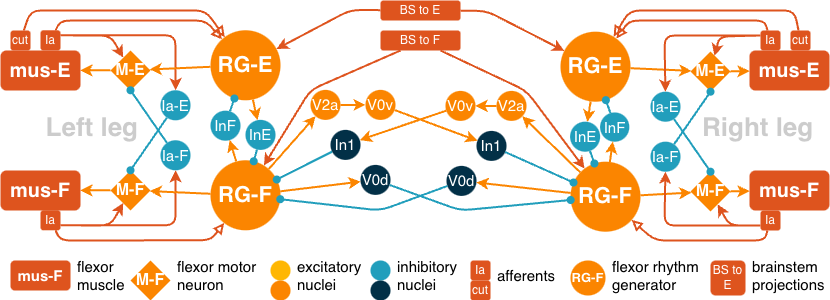
\includegraphics[width=0.8\textwidth]{fig1_schematic.png}
  \caption{\textbf{Architecture of the two-leg spinal CPG.}
    Each leg contains a flexor (F)
    and extensor (E) rhythm-generator half-centre coupled by asymmetric
    reciprocal inhibition via InE and InF interneurons (Zhang 2022 6:1
    ratio). Sensory afferents (Ia, cutaneous) feed into the
    reciprocal-inhibition interneurons; motor pools (M-E, M-F) drive
    muscle proxies whose force and length signals close the Ia loop.
    L\,$\leftrightarrow$\,R commissural inhibition (V0-like) is mediated by
    flexor- and extensor-targeted projections.}
  \label{fig:schematic}
\end{figure}

\subsection{Single-neuron model}\label{sec:methods:neuron}
The network is implemented at two complementary levels of biophysical
detail, using the same architecture, the same plastic projections and the
same experimental protocol in both cases.

\paragraph{Reduced (Izhikevich) implementation.}
In the NEST implementation, all spiking neurons are modelled as Izhikevich
quadratic-integrate-fire units~\cite{izhikevich2003}. Each neuron obeys
\begin{align}
  \frac{dv}{dt} &= 0.04v^2 + 5v + 140 - u + I, \\
  \frac{du}{dt} &= a\,(bv - u),
\end{align}
with the after-spike reset $v \leftarrow c$, $u \leftarrow u + d$ applied
whenever $v \geq 30$\,mV. Excitatory extensor RG-E neurons use the
regular-spiking set ($a=0.02, b=0.2, c=-65, d=8$). Flexor RG-F neurons use
the intrinsically-bursting set ($a=0.02, b=0.2, c=-55, d=4$), which
approximates persistent-sodium-driven ($I_\text{NaP}$) bursting
phenomenologically rather than deriving it from channel kinetics.
Inhibitory interneurons (InE, InF, Ia-INT) use a fast-spiking set
($d=2$). This formulation reproduces the spiking and bursting regimes
required by the rhythm generator at a small fraction of the computational
cost of a conductance-based model, which is what makes the large
mode\,$\times$\,learning-rate parameter sweeps reported here tractable.

\paragraph{Conductance-based (Hodgkin--Huxley) implementation.}
Because the reduced model represents bursting phenomenologically, we also
implemented the same circuit with conductance-based neurons in
NEURON~\cite{hines1997}, following the Hodgkin--Huxley
formalism~\cite{hodgkinHuxley1952}. Membrane potential evolves as
\begin{equation}
  C_m \frac{dV}{dt} = -\!\sum_i g_i\, m_i^{p}h_i^{q}\,(V - E_i) - I_\text{leak} + I_\text{syn},
  \label{eq:hh}
\end{equation}
where each active conductance $g_i$ is gated by activation ($m_i$) and
inactivation ($h_i$) variables obeying first-order kinetics
$\dot{x} = (x_\infty(V) - x)/\tau_x(V)$. Rhythm-generator neurons include
fast sodium, delayed-rectifier potassium and leak conductances together
with an explicit persistent sodium current ($I_\text{NaP}$), so that
bursting arises from channel kinetics rather than from a reset rule.
Motoneurons and interneurons are multi-compartment cells with somatic and
dendritic sections. This implementation resolves the sub-threshold and
channel-level dynamics that the Izhikevich formulation abstracts away, at
substantially higher computational cost; it therefore serves as a
biophysical cross-check on the reduced model rather than as the vehicle
for the full parameter sweep.%
\todo{The NEURON/HH results are not yet included in Results. Until they
are, this subsection describes an implementation the paper does not yet
report on, and the Limitations no longer flag the absence of a
conductance-based model --- add the HH results (or re-scope this
paragraph) before circulating.}

Synaptic delays in both implementations are drawn from a rat
\texttt{length\_velocity} preset (Table~\ref{tab:delays}) with
$\sigma=0.2$\,ms Gaussian jitter.

\subsection{Network architecture}\label{sec:methods:network}

\paragraph{Asymmetric reciprocal inhibition (Zhang 2022).}
The F$\to$InF$\to$E pathway is strong ($W_{\text{InF}\to\text{RG-E}}=-48$\,pA,
$P=0.30$); the E$\to$InE$\to$F pathway is weak
($W_{\text{InE}\to\text{RG-F}}=-8$\,pA, $P=0.15$).
The 6:1 ratio preserves the flexor's role as the rhythm-leading
half-centre~\cite{zhang2022,talpalar2013}.

\paragraph{Closed-loop Ia$\to$reciprocal-IN pathway (this work).}
Ia-E parrots project to InE ($W=6$\,pA, $P=0.25$) and Ia-F parrots to
InF, providing closed-loop sensory drive into the reciprocal-inhibition
core. This pathway compensates the loss of strong tonic descending drive
characteristic of deafferented fictive locomotion~\cite{pearson1995,
rossignol2006,hultborn2006}.

\paragraph{Cutaneous reflex.}
Cutaneous parrots project to RG-E (STDP-plastic) and to InE
($W=6$\,pA, $P=0.30$), implementing the stance-phase cutaneous-reflex
gating of extensor activity~\cite{forssberg1980,pearson1995}.

\paragraph{Commissural inhibition.}
L$\leftrightarrow$R flexor RG inhibition is strong
($W=-20$\,pA, $P=0.22$); extensor inhibition is weak
($W=-8$\,pA, $P=0.10$). This V0-mediated commissural inhibition
enforces left--right alternation~\cite{kiehn2016,talpalar2013}.

\paragraph{Motor pool, muscle relay.}
Each motor neuron projects to $N_{\text{mus}}=100$ muscle-parrot relays
($P_{\text{M}\to\text{mus}}=0.8$). Motor pool reciprocal inhibition
($W=-22$\,pA, $P=0.25$) enforces antagonist suppression at the motor
level~\cite{mccreaRybak2008}.

\paragraph{Connectivity specification.}
The full per-connection weight and delay distributions of every
projection were obtained by querying NEST directly after network
construction. Table~\ref{tab:delays}
lists all projections grouped by the functional blocks of the
architecture (Fig.~\ref{fig:schematic}): descending/supraspinal drive,
the sensory afferent$\to$RG projections, the rhythm-generator reciprocal
core, the Ia proprioceptive interneuron pathway, motor output, and the
commissural (interlimb) projections. Static projections are
heterogeneous: their per-connection weights are drawn from a lognormal
distribution about the design value (coefficient of variation $0.5$, mean
and sign preserved), since biological synaptic weights are lognormally
distributed rather than uniform~\cite{song2005,buzsaki2014}. The mean
preserves the designed balance---in particular the asymmetric reciprocal
inhibition (InF$\to$RG-E $=-48$\,pA, InE$\to$RG-F $=-8$\,pA) reproduces the
Zhang~6:1 ratio exactly. The plastic projections (CUT$\to$RG-E in both
arms, BS$\to$RG in the descending arm, Ia$\to$RG in the sensory arm) carry
lognormal weight distributions from STDP: the table reports their
\emph{converged} mean$\pm$s.d.\ (CUT$\to$RG-E and Ia$\to$RG at their
learned load set-points, BS$\to$RG frozen at weak init in the sensory
arm). The cutaneous input to RG-E is a single plastic projection. Conduction delays follow the rat
\texttt{length\_velocity} preset (brainstem pathways $\approx 3.0$\,ms,
reciprocal and motor pathways $\approx 1.8$\,ms, commissural
$\approx 2.2$\,ms) with $0.2$\,ms across-connection jitter. The
muscle$\to$Ia spindle/GTO feedback is implemented as a rate-coded
transduction (force and length $\to$ Ia firing rate), not a synaptic
projection, and so has no weight/delay entry.
Figure~\ref{fig:connectivity} shows the weight and delay distributions.


\begin{figure}[t]
  \centering
  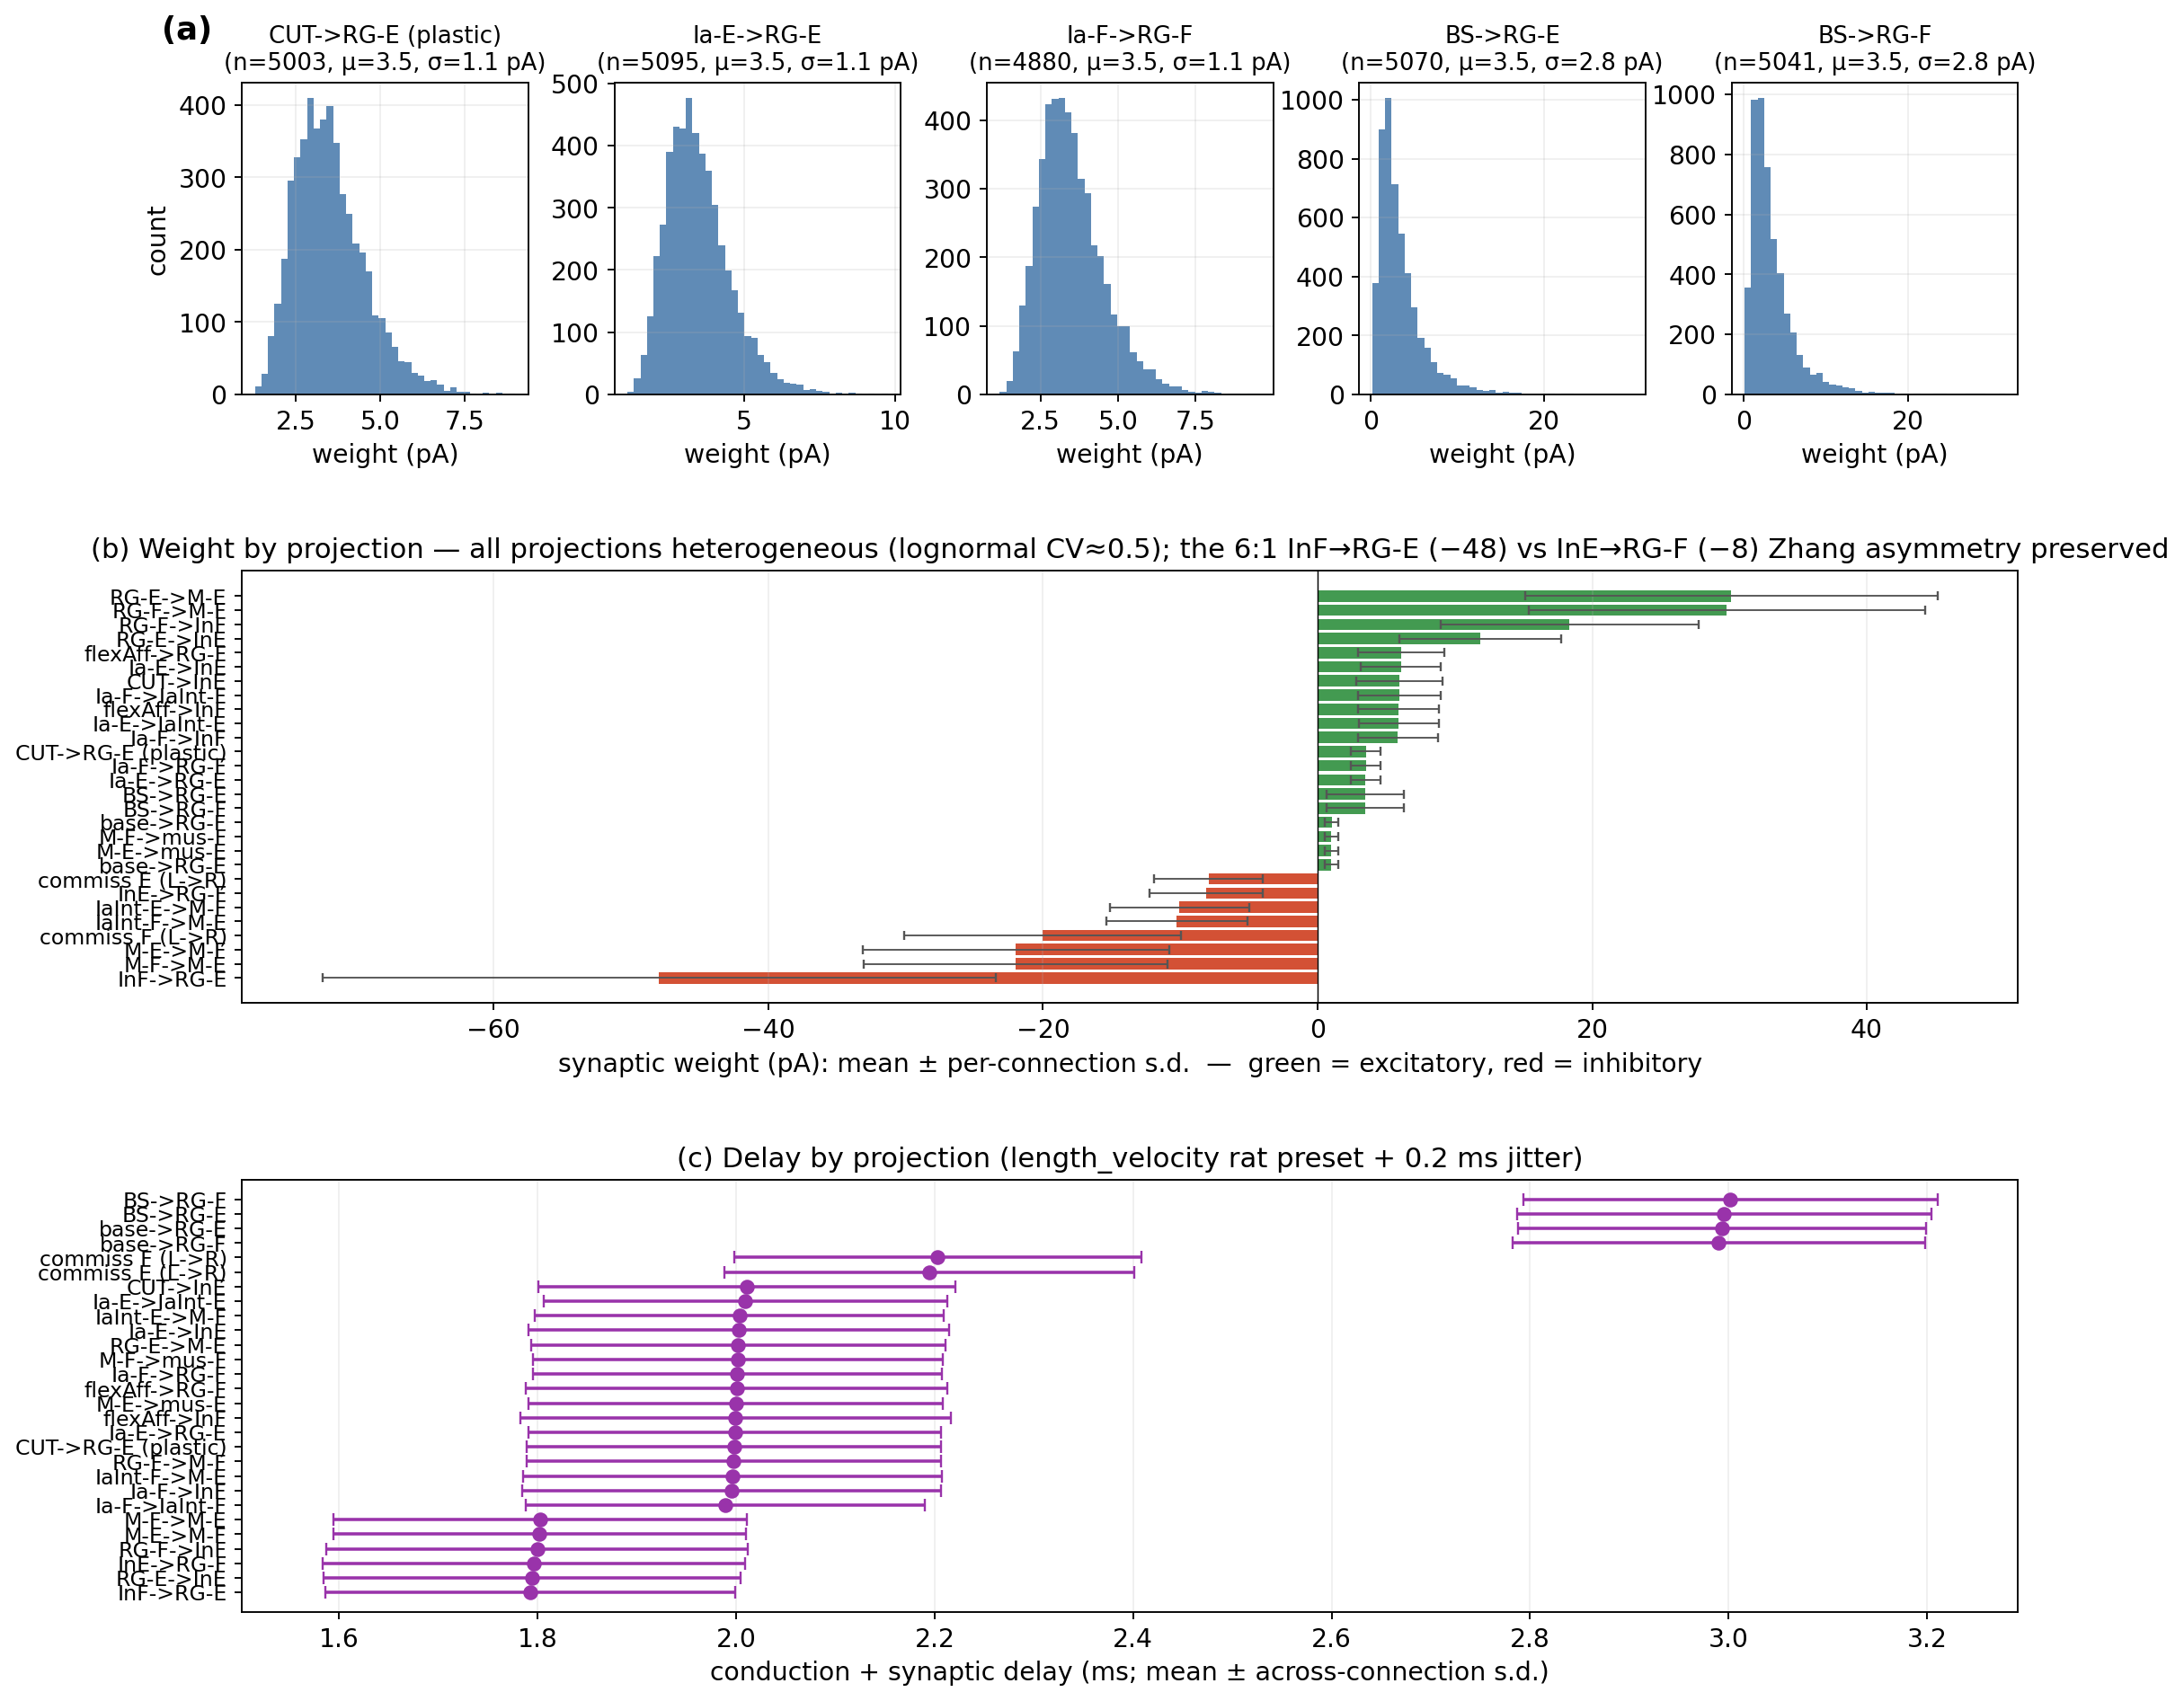
\includegraphics[width=0.8\textwidth]{fig_connectivity.png}
  \caption{Distribution of synaptic weights and conduction delays along
  every projection (sensory-arm configuration: frozen BS$\to$RG, plastic
  Ia$\to$RG). \textbf{(a)} Weight histograms for the plastic / learned
  projections (STDP + lognormal init). \textbf{(b)} Synaptic weight per
  projection (mean $\pm$ per-connection s.d.; green excitatory, red
  inhibitory) --- all projections are heterogeneous (lognormal, CV$\approx
  0.5$), with the asymmetric reciprocal inhibition InF$\to$RG-E $=-48$\,pA
  versus InE$\to$RG-F $=-8$\,pA preserving the Zhang~6:1 ratio in the mean.
  \textbf{(c)} Conduction~+~synaptic delay per projection (mean $\pm$
  across-connection s.d.), following the rat \texttt{length\_velocity}
  preset with $0.2$\,ms jitter.}
  \label{fig:connectivity}
\end{figure}

\subsection{Brainstem drive}\label{sec:methods:bs}
Reticulospinal input is modelled as a tonic Poisson process at
$BS_{\text{regular}}=60$\,Hz with $\sigma=0.25$\,Hz noise, identical for
both legs. The 60\,Hz value sits in the
middle of the rat reticulospinal range
(20--80\,Hz)~\cite{drew1986,brocard2010}. In contrast to~\cite{zhang2022},
who vary tonic drive $\alpha$ to vary gait speed, we hold BS tonic and
pace the rhythm via sensory feedback (see \autoref{sec:methods:paced}).

\subsection{Spike-timing-dependent plasticity}\label{sec:methods:stdp}
Two projections --- cutaneous CUT$\to$RG-E and brainstem
BS$\to$RG-\{E,F\} --- carry multiplicative STDP synapses (NEST
\verb|stdp_synapse|; $\tau_+=20$\,ms, default $\lambda=10^{-3}$,
$\alpha=0.95$, $\mu_+=\mu_-=0.4$, $w_{\max}=120$\,pA for CUT and
$w_{\max}=30$\,pA for BS)~\cite{biPoo1998,morrison2007}. Initial
weights are drawn from a lognormal distribution with mean $\mu$ and
coefficient of variation CV. We swept $(\mu,\text{CV})$ across ten
diagnostic points (the ten $(\mu,\mathrm{CV})$ initialisation points) spanning four orders of
magnitude to verify that the post-training weight distribution
converges to the same plateau regardless of initialisation (see
Section~\ref{sec:results:weights}).

\paragraph{Extensor-biased plasticity and stance/swing asymmetry.}
The plastic and paced drives are deliberately extensor-weighted, mirroring
the stance/swing organisation of locomotor control. The cutaneous
afferent --- the only projection with the large ($w_{\max}=120$\,pA)
plasticity ceiling --- targets the extensor (CUT$\to$RG-E) and has no
flexor counterpart, reflecting that paw-contact cutaneous feedback fires
during weight-bearing stance and reinforces the load-bearing
extensor~\cite{pearson1995,rossignol2006}. Likewise the paced
heel$\to$toe Ia-E ramp clocks the extensor during stance, whereas the
flexor receives no external pacing and is generated intrinsically ---
by the persistent-sodium-like bursting of the RG-F units and by release
from reciprocal inhibition during swing. As a consequence the extensor
half-centre is sensory-driven and tightly clocked while the flexor is
centrally generated and intrinsically more variable; and because the
dominant plastic projection is extensor-only, increasing $\lambda$
strengthens the descending drive asymmetrically, in favour of the
extensor (analysed in Section~\ref{sec:results:force}).

\paragraph{Learning-rate variation.}
For the speed-by-STDP and graded-ablation matrices
(\autoref{sec:methods:protocols}), the STDP learning rate $\lambda$ was
varied across three values spanning two decades at and below the
cortical bio-plausible STDP rate~\cite{biPoo1998,morrison2007}:
$\lambda \in \{1{\times}10^{-5},\,1{\times}10^{-4},\,1{\times}10^{-3}\}$.
We refer to these as \emph{slow}, \emph{intermediate}, and
\emph{baseline} STDP, respectively. With a 120\,s run the slow rate does
not fully converge (time constant $\approx 250$\,s), which lets us probe
the regime of weak, still-developing descending weights. The parameter
is recorded to the simulation output for every run.

\subsection{Sensory feedback and Ia rate coding}\label{sec:methods:ia}
Ia afferent firing rate $r_{\text{Ia}}$ is updated every 100\,ms as a
linear combination of muscle force $F$ and stretch $\Delta\ell$:
\begin{equation}
  r_{\text{Ia}} = r_0 + k_F \cdot F + k_S \cdot \max(0, \ell - L_0),
  \quad \text{clamped to } [0, r_{\max}],
  \label{eq:ia}
\end{equation}
with $r_0=10$\,Hz, $k_F=6$\,Hz/F, $k_S=250$\,Hz/L,
$r_{\max}=500$\,Hz~\cite{loeb1981,prochazka1999}. This rate drives the
classical Ia-INT$\to$antagonist motor-pool
pathway~\cite{jankowska1992} and the closed-loop Ia$\to$recip-IN pathway
introduced in this work.

\paragraph{Graded sensory ablation (Courtine/Lavrov paradigm).}
To emulate the partial-weight-bearing and limb-unloaded preparations
used in rat SCI rehabilitation
experiments~\cite{lavrov2008,courtine2009,edgerton2008}, we expose a
multiplicative Ia-feedback gain $G_{\text{Ia}} \in [0, 1]$, applied
after Eq.~\ref{eq:ia}:
$\tilde{r}_{\text{Ia}} = G_{\text{Ia}}\cdot r_{\text{Ia}}$. The three
operating regimes used in Section~\ref{sec:results:epidural} are:
$G_{\text{Ia}}=1.0$ (\emph{baseline}, full weight-bearing);
$G_{\text{Ia}}=0.5$ (\emph{toe stepping}, partial weight); and
$G_{\text{Ia}}=0.1$ (\emph{air stepping}, limb unloaded, residual
spindle background only). The classical Ia-INT$\to$antagonist pathway
inherits the same gain, so the manipulation reduces \emph{all} Ia
output uniformly.

\subsection{Activation and force dynamics}\label{sec:methods:muscle}
The muscle relay rate $r_{\text{mus}}$ is mapped to activation $a$
through a saturating nonlinearity gated by RG-rate. The gate is a smooth
logistic (sigmoid) of the normalised RG population rate --- a
bio-plausible soft saturation in place of a hard clip:
\begin{align}
  a_{\text{raw}} &= a_{\max} \, \bigl(1 - \exp(-k_a \, r_{\text{mus}})\bigr), \label{eq:araw}\\
  d &= \sigma\!\Bigl(k_g\bigl(r_{\text{RG}}/r_{\text{ref}} - x_0\bigr)\Bigr),
       \qquad \sigma(z)=\frac{1}{1+e^{-z}}, \label{eq:gate}\\
  a_{\text{tgt}} &= a_{\text{raw}} \cdot d, \label{eq:atgt}\\
  a(t+\Delta t) &= a(t) + \bigl(1 - e^{-\Delta t/\tau_a}\bigr)\bigl(a_{\text{tgt}} - a(t)\bigr).
  \label{eq:alp}
\end{align}
with gate steepness $k_g=8$ and mid-point $x_0=0.6$. The logistic
saturates smoothly at $1$ and suppresses the inter-burst trough
($d\approx0.06$ at $r_{\text{RG}}/r_{\text{ref}}\approx0.25$ versus
$d\approx0.83$ at a burst peak), so the gated target $a_{\text{tgt}}$ is
bounded in $[0,a_{\max})$ by construction --- without the hard clip used
in earlier versions of the model.
Force follows an identical first-order low-pass driven by a saturating
function of activation:
\begin{align}
  F_{\text{tgt}} &= F_{\max} \, \bigl(1 - \exp(-k_F \, a)\bigr),\\
  F(t+\Delta t) &= F(t) + \bigl(1 - e^{-\Delta t/\tau_F}\bigr)\bigl(F_{\text{tgt}} - F(t)\bigr).
\end{align}
Under the paced-gait protocol (\autoref{sec:methods:paced}) the time
constants are overridden: $\tau_a=40$\,ms, $\tau_F=80$\,ms. The latter
sits within the rat fast-twitch fibre rise-time
range~\cite{zajac1989,winters1995}.

\paragraph{Force units and SI calibration.}
Force is reported in arbitrary units (a.u.). The dimensionless ceiling
$F_{\max}=25$\,a.u.\ in Eq.~(6) was chosen so the activation--force
cascade operates in a numerically convenient range; absolute Newton
calibration is not intrinsic to the present model and is conventional
in CPG-modelling reports~\cite{rybak2006,danner2017,zhang2022}. A
first-order linear rescaling maps a.u.\ to Newtons by anchoring on
\emph{in vivo} rat hindlimb data: the peak isometric tetanic force of
rat medial gastrocnemius is approximately
$5$--$7$\,N~\cite{roy1991,burkholderLieber2001}. Treating our reported
peak Force-E of $17.4$\,a.u.\ as representing peak ankle-extensor
tetanic force gives a conversion of $1$\,a.u.\ $\approx$
$0.30$--$0.40$\,N. Nothing in the model dynamics depends on this
choice of units; we use a.u.\ throughout for transparency.

\subsection{Paced gait protocol}\label{sec:methods:paced}
Each step period (default 1000\,ms) is divided
into two 500\,ms half-cycles. During the stance half of leg L, the L
cutaneous generator fires at $CUT_{\text{on}}=100$\,Hz, and three
sequential Ia-E sub-groups fire at 60, 80, and 100\,Hz over consecutive
$\sim$167\,ms windows, emulating heel$\to$mid$\to$toe pressure transfer
during stance~\cite{loebDuysens2018}. During swing, all CUT and Ia-E
drive is silenced. The contralateral leg R follows the 180\,$^{\circ}$
mirror schedule (trot pattern). Reciprocal inhibition and the RGF
intrinsic-bursting dynamics maintain the swing-leg flexor burst without
external pacing.

\subsection{Simulation setup}\label{sec:methods:sim}
All simulations were performed with NEST~3.9~\cite{nest2002} using a
kernel resolution of 0.2\,ms, simulation chunks of 100\,ms, and 64
OpenMP threads per task on a single AMD EPYC node (MN5 system,
Barcelona Supercomputing Center). Initial-weight sweeps were run as
10-task SLURM job arrays; ablation and speed-sweep experiments used
5-task arrays. A 30\,s simulation completes in $\sim$30\,min wall-clock;
a 120\,s simulation in $\sim$2\,h.

\subsection{Experimental protocols}\label{sec:methods:protocols}
Three classes of in-silico experiments are reported in this paper. Each
is encoded as a stand-alone shell script that submits a single
multi-task SLURM array and writes one HDF5 file per array task.
Pseudocode for all three is given in the Supplementary material (Algorithms~\ref{alg:main}--\ref{alg:ablgrad}).

\paragraph{Main experiment: long-term self-organisation.}
A 10-point sweep over the initial-weight distribution $(\mu,\mathrm{CV})$
for the STDP synapses, run as a SLURM job array. Each task simulates
\SI{120}{\second} of paced locomotion at $\mu, \mathrm{CV}$ drawn from
the ten $(\mu,\mathrm{CV})$ initialisation points. Used in Section~\ref{sec:results:weights}.


\paragraph{Phase A --- speed-by-STDP matrix.}
Nine 120\,s runs spanning three walking speeds (rat locomotor range,
\cite{lavrov2008,courtine2009}) crossed with three bio-plausible STDP
learning rates. Used in Section~\ref{sec:results:force}.


\paragraph{Phase B --- graded sensory ablation by STDP matrix
(Courtine/Lavrov SCI paradigm).}
Nine 120\,s runs at the medium-walk anchor ($P=520$\,ms) crossing three
Ia feedback gains with three STDP rates. Used in
Section~\ref{sec:results:epidural}.


\paragraph{Legacy ablation experiment (supplementary).}
For completeness we retain the earlier 5-condition ablation experiment
(\emph{baseline}, \emph{noIa}, \emph{symInh}, \emph{noComm},
\emph{noPaced}) that demonstrated which architectural components are
load-bearing. The Phase B graded ablation is the principal ablation
result of the paper; the binary ablation is reported in supplementary
Fig.~S1.

\noindent All three scripts (\texttt{run.sh}, \texttt{run\_ablation.sh},
\texttt{run\_speed.sh}) are publicly available in the repository. Each
single 30\,s task runs in $\sim$30\,min wall-clock on a 64-thread MN5
node; the 120\,s task takes $\sim$2\,h. Total compute for all three
experiments: $\sim$60 core-hours.

\subsection{Data analysis}\label{sec:methods:analysis}
Cycle period was computed as the Force-E peak-to-peak interval over the
last 20\,s, using a 5\,a.u.\ minimum peak height and a 300\,ms minimum
inter-peak gap. Counter-phase strength was reported as Pearson's
correlation between Force-E and Force-F over the same window. Peak
force amplitude was reported as the 95th percentile to avoid outlier
sensitivity. STDP convergence was reported as the per-projection mean
$\pm$ standard deviation of synaptic weights sampled every 1\,s. No
formal statistical tests are reported: simulations are deterministic with
a fixed seed (12345 + 10007$\times$idx for sweep tasks); reproducibility
is therefore exact, and uncertainty is captured by the $(\mu,\text{CV})$
initialisation sweep rather than by stochastic repetition.

% --- Parameter tables go in supplementary ---


\section{Results}\label{sec:results}
% Results — figure-driven description on the 5 locomotion modes x 3 STDP rates
% ("rehabilitation modes") of the canonical sensory-sited model.
%   fig_stdp_weight_matrix   = weights, both legs x 3 projections x 5 modes
%   fig_stdp_weights_grid    = weights, 5 modes x 3 lambda (3 projections/panel)
%   fig_force_stages_lam*    = force at 3 learning stages, 5 modes, per lambda
%   fig_network_matrix_lam*  = 16 population rates x 5 modes, per lambda
%   fig9_epidural_contrast   = epidural-stim vs natural loading contrast

Before the individual results we fix the terms used throughout. The model is a
two-legged spinal CPG: a spiking network that,
driven only by a weak tonic brainstem input and rhythmic sensory feedback,
produces the alternating extensor/flexor muscle activity of walking. Each leg
contains two mutually-inhibiting neuron pools --- an \emph{extensor} and a
\emph{flexor} rhythm generator (RG-E and RG-F) --- that drive motor neurons and
simple muscle models. A good walking rhythm is one in which extensor and flexor
are active in strict alternation (``counter-phase''); we measure this by the
Pearson correlation between the two muscle forces, which is $-1$ for perfect
alternation and $0$ for none. Three synapses in the model are \emph{plastic} ---
their strengths change as the network runs, through STDP. The Results ask
how this self-tuning builds the gait, and how
well the learned gait survives when sensory feedback is progressively removed,
as it is in spinal-cord-injury rehabilitation.

\subsection{The network tunes its own synapses to a stable set-point}\label{sec:results:weights}

\paragraph{The model and its $5\times5$ grid of test conditions.}
We place the learning in the sensory pathways and hold the brainstem input
fixed, so the three plastic synapses are: the cutaneous CUT$\to$RG-E projection
(paw-contact skin feedback onto the extensor generator) and two proprioceptive
projections, Ia-E$\to$RG-E and Ia-F$\to$RG-F (muscle-stretch feedback onto the
matching generator). Every result is reported on the same grid crossing
\emph{five locomotion modes} with \emph{five learning rates}. The locomotion
modes span a rehabilitation continuum: slow, medium and fast walk (6, 13.5 and
21\,cm/s, all at full weight-bearing --- medium walk is also called
\emph{plantar stepping} or \emph{baseline}), then \emph{toe stepping} (partial
body-weight support) and \emph{air stepping} (the limb fully unloaded, as when a
spinal rat is suspended). The learning rate $\lambda$ sets how much each plastic
synapse changes per correlated pre/post spike pair --- larger $\lambda$ means
faster learning --- and we sweep it across five decades,
$\lambda\in\{10^{-2},10^{-3},10^{-4},10^{-5},10^{-6}\}$.

\paragraph{The synapses grow, then settle at values that do not depend on the
walking mode.}
Starting from weak random values, STDP drives each plastic synapse to a steady
strength and holds it there (Figure~\ref{fig:weight_matrix}). The cutaneous
CUT$\to$RG-E synapse grows strong --- to $\approx63$\,pA --- in every
weight-bearing mode, whereas the two proprioceptive synapses settle at a low
$\approx4$--$5$\,pA, well below their $10$\,pA ceiling. This low set-point is
functionally important: a light, correctly-timed proprioceptive input reinforces
each burst without ``filling in'' the silent gap between bursts, which would
otherwise abolish the alternation. The left and right legs learn identical
values.

\begin{figure}[t]
  \centering
  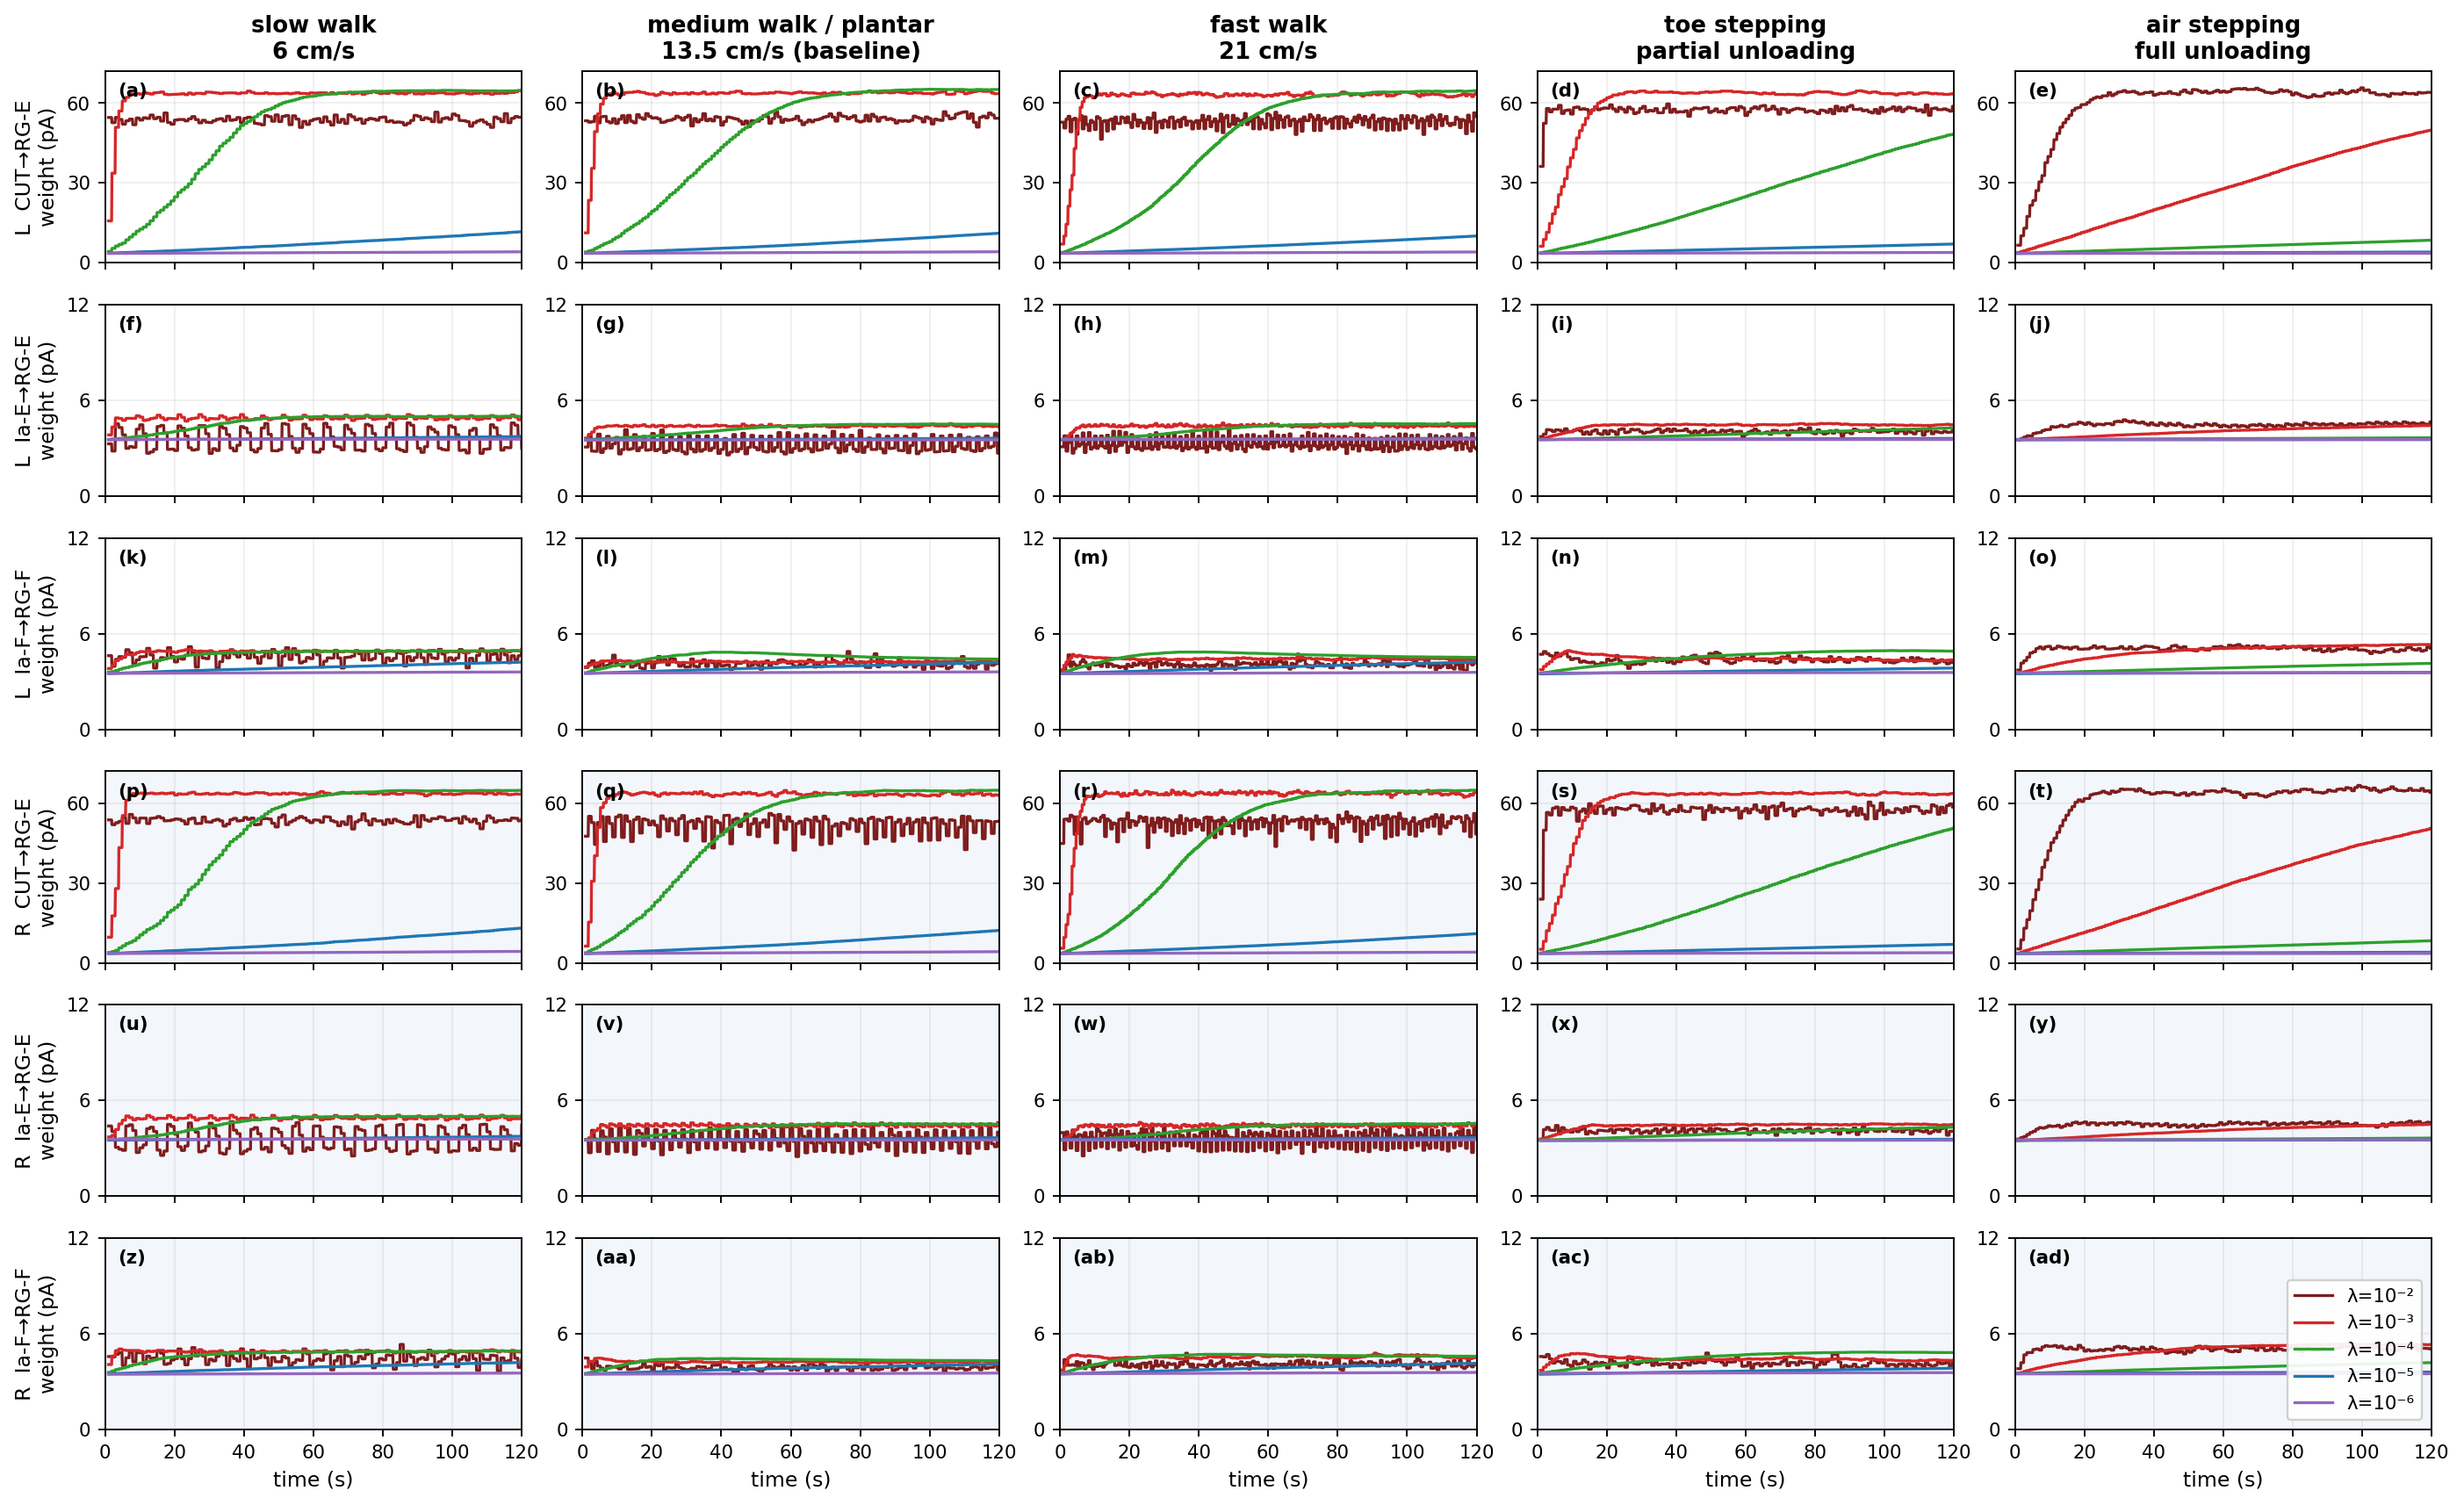
\includegraphics[width=0.92\textwidth]{fig_stdp_weight_matrix.png}
  \caption{\textbf{STDP weight trajectories of the three plastic projections
    across the five locomotion modes.} Rows: CUT$\to$RG-E, Ia-E$\to$RG-E,
    Ia-F$\to$RG-F for the left leg (white) then the right leg (tinted); columns:
    slow~/ medium\,$=$\,plantar\,$=$\,baseline / fast walk and toe / air
    stepping. Each panel overlays the three learning rates $\lambda$. Weight
    (pA) versus time (s). CUT$\to$RG-E converges to $\approx63$\,pA in every
    mode; the two proprioceptive projections self-stabilise at a low
    $\approx4$--$5$\,pA set-point; the two legs are symmetric.}
  \label{fig:weight_matrix}
\end{figure}

\paragraph{The learning rate sets only how fast the synapse settles; unloading
slows it.}
Faster learning reaches the plateau sooner (Figure~\ref{fig:weights_grid}):
CUT$\to$RG-E settles within $\approx7$\,s at $\lambda=10^{-3}$, but takes
$\approx75$\,s at $10^{-4}$ and has not finished settling within the $120$\,s run
at $10^{-5}$. Removing body-weight support slows learning further, because the
paw-contact feedback that drives the synapse is itself weakened when the limb is
unloaded: under air stepping even the fastest rate climbs only gradually (to
$\approx50$\,pA by the end of the run). The proprioceptive synapses stay at
their low set-point in every condition.

\begin{figure}[t]
  \centering
  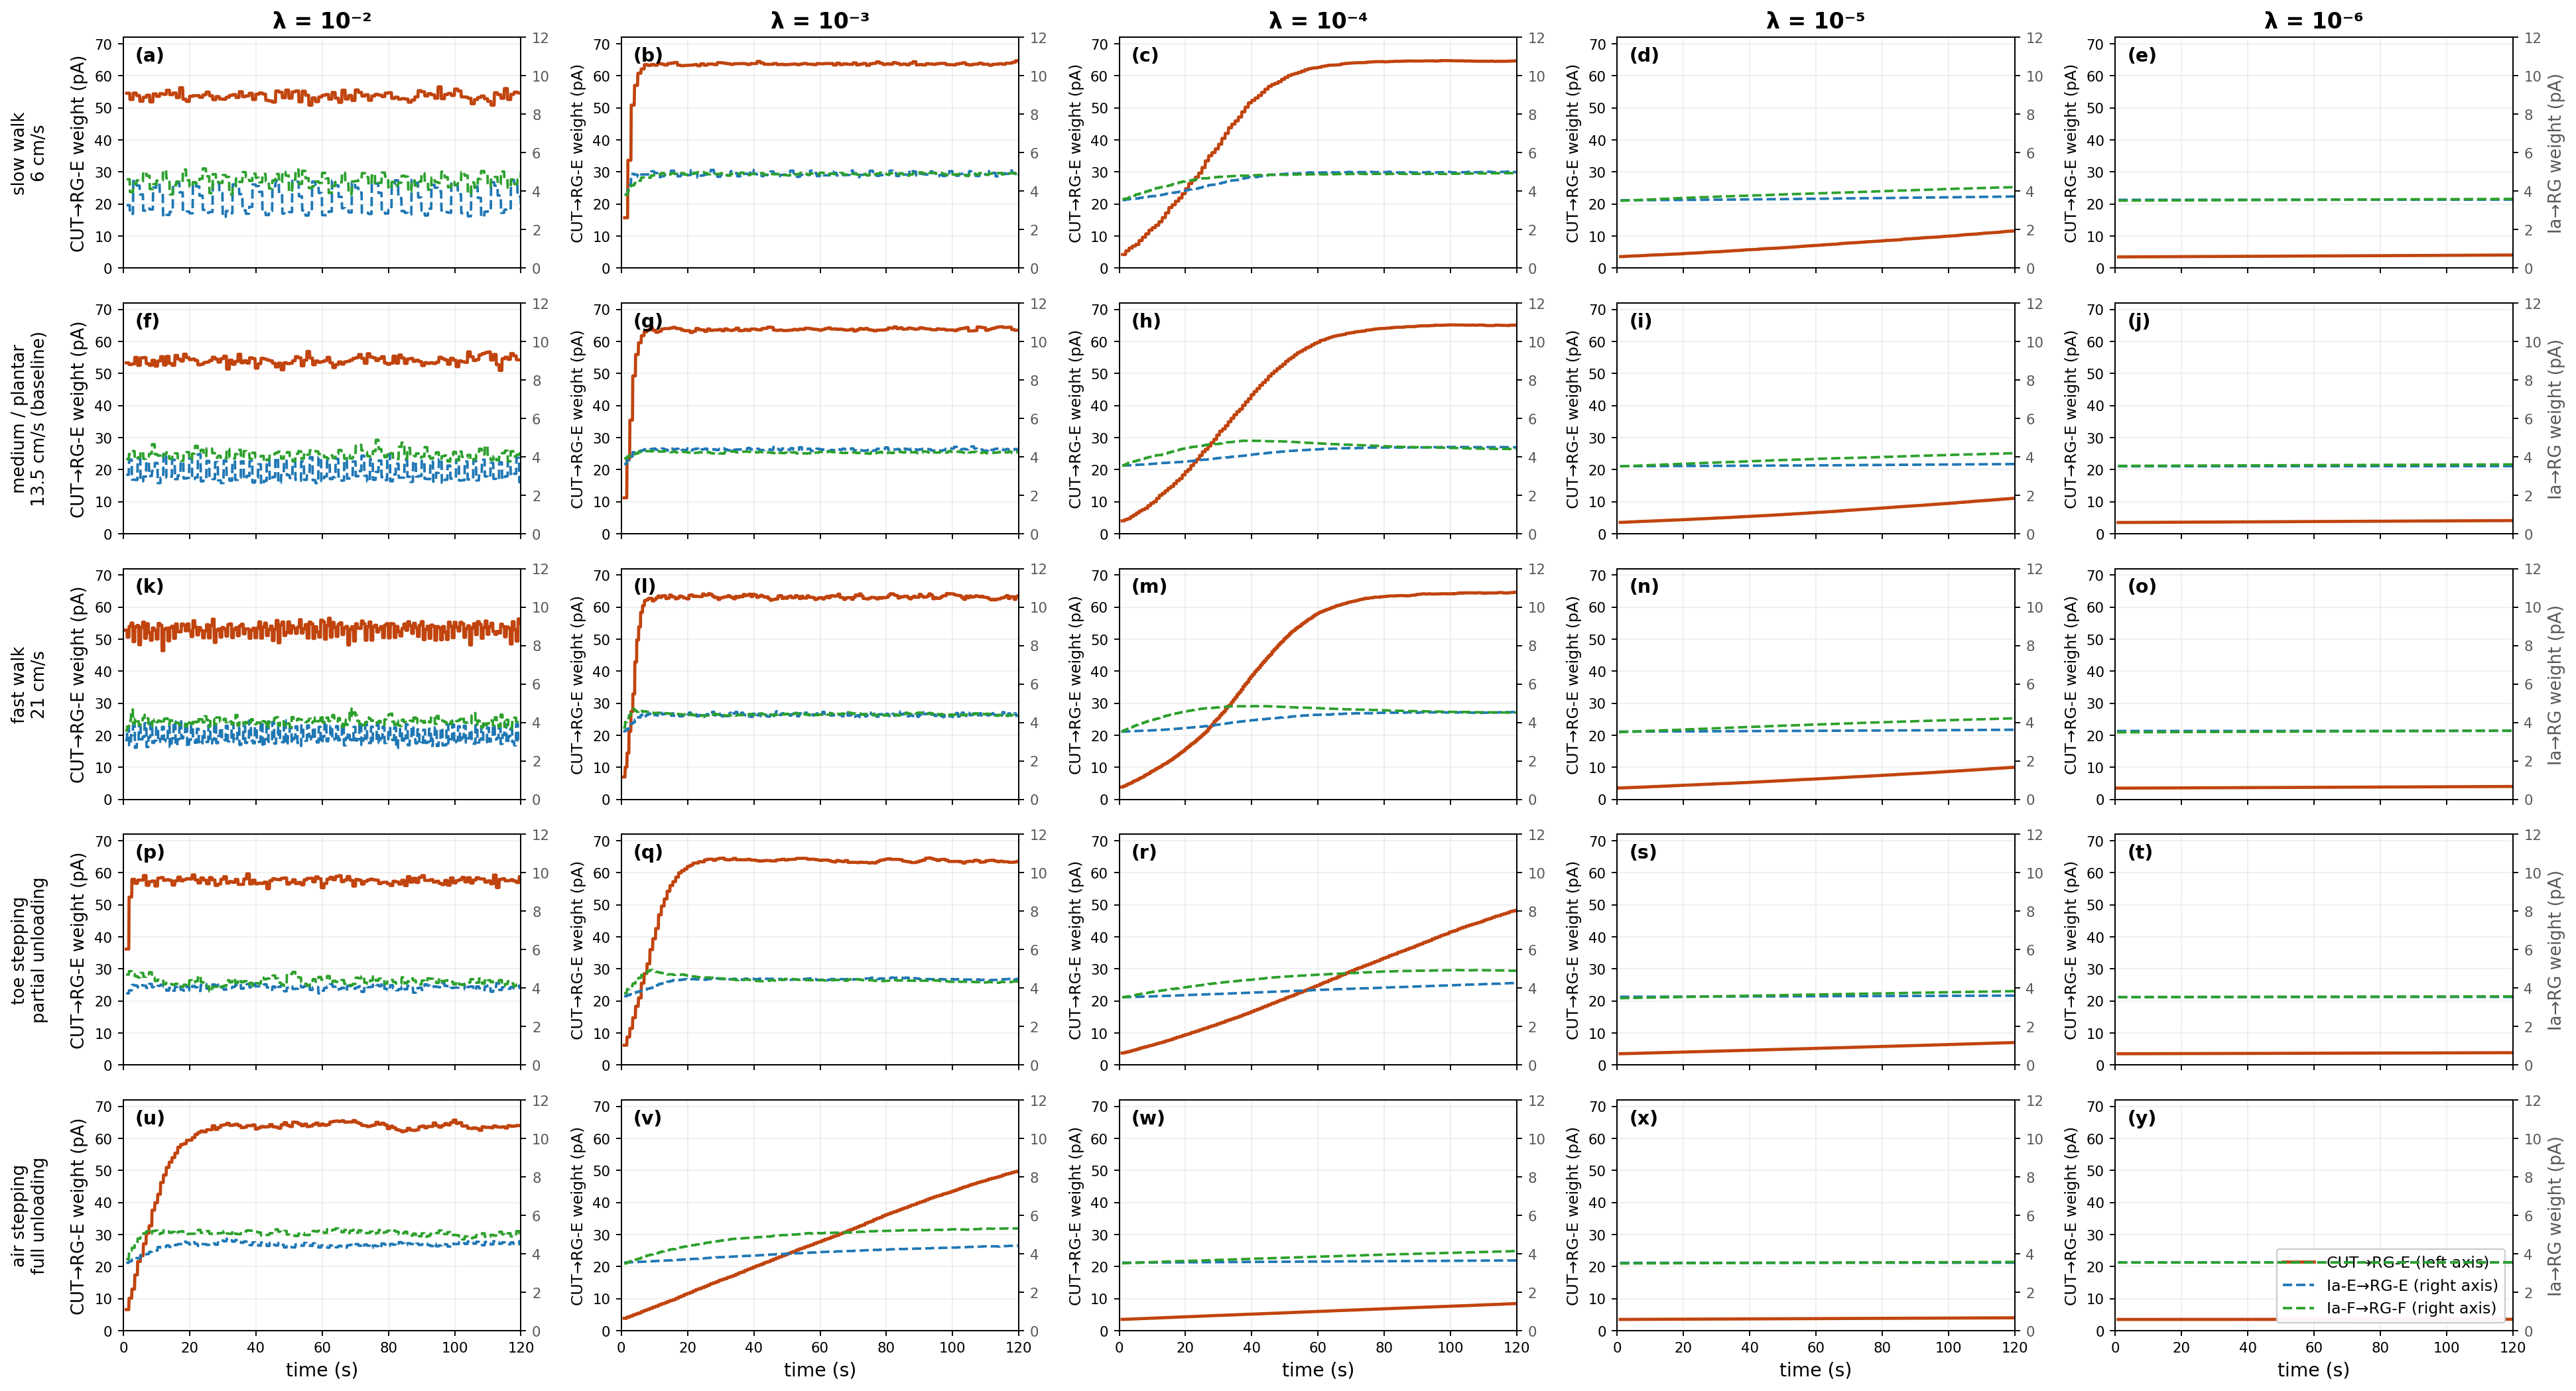
\includegraphics[width=0.92\textwidth]{fig_stdp_weights_grid.png}
  \caption{\textbf{Weight trajectories of all three plastic projections, per
    rehabilitation mode.} Rows: the five locomotion modes; columns: the three
    learning rates. Each panel shows CUT$\to$RG-E (solid, left axis, pA) and the
    two proprioceptive projections Ia-E$\to$RG-E and Ia-F$\to$RG-F (dashed, right
    axis, pA) versus time (s). Panels (a)--(y). The learning rate sets the
    time-to-plateau; unloading (bottom rows) slows CUT$\to$RG-E convergence.}
  \label{fig:weights_grid}
\end{figure}

% =============================================================
\subsection{Rehabilitation progress: force develops as the weight converges}\label{sec:results:force}

We next examine whether this self-tuned wiring produces good walking, and how
the gait builds up over a session. Figures~\ref{fig:force_l2}--\ref{fig:force_l6} show the
extensor and flexor muscle forces in three short windows --- the beginning,
middle and end of each $120$\,s run --- so that reading a figure left-to-right
traces how the gait develops as the synapse strengthens (one figure per learning
rate). Early in the run the two forces overlap in ragged, poorly-timed bursts;
as CUT$\to$RG-E grows they separate into a clean alternation. At the fast and
intermediate rates ($\lambda=10^{-2}$ to $10^{-4}$) the synapse converges within
the run and the weight-bearing modes reach near-perfect counter-phase (muscle-%
force correlation down to $-0.99$, where $-1$ is ideal). Toe stepping is clean at
the faster rates but degrades as learning slows (correlation $-0.96$ at $10^{-2}$
down to $-0.39$ at $10^{-6}$), and air stepping never exceeds $\approx-0.55$ at
any rate, because with the limb unloaded the extensor synapse stays weak
($\approx4$\,pA). At the two slowest rates ($\lambda=10^{-5},10^{-6}$) the synapse
barely develops within $120$\,s, so the gait stays under-formed from beginning to
end.

\begin{figure}[t]
  \centering
  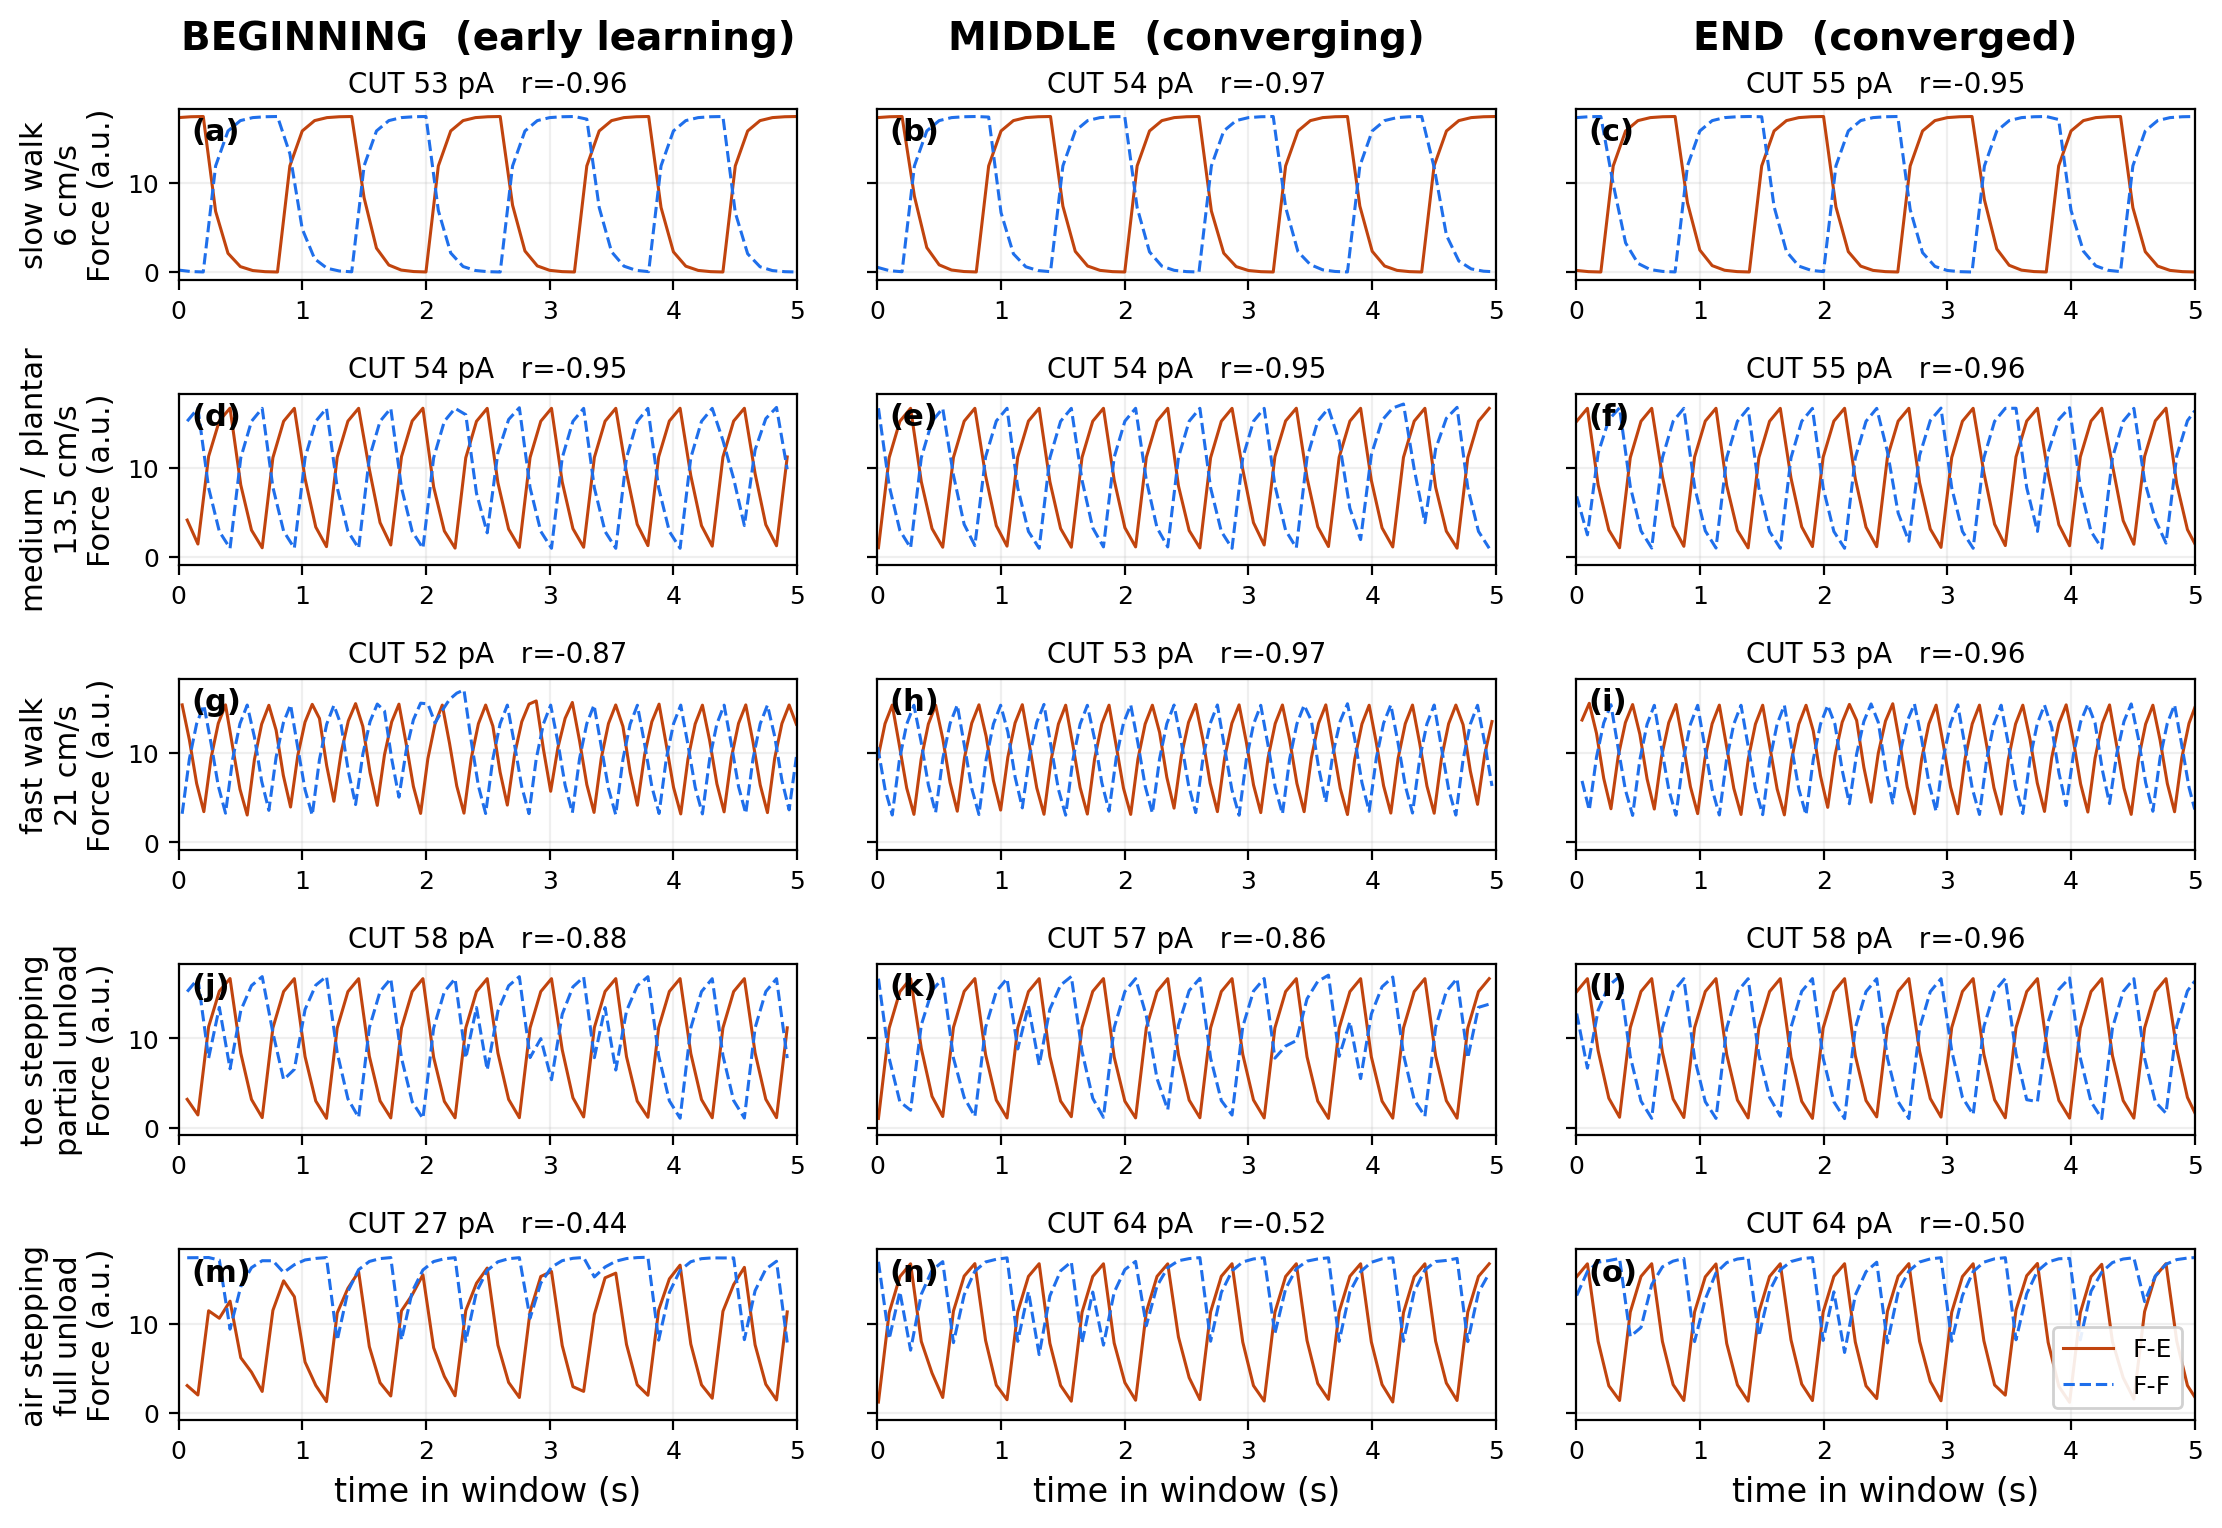
\includegraphics[width=0.9\textwidth]{fig_force_stages_lam1em2.png}
  \caption{\textbf{Force at three learning stages, five locomotion modes,
    $\lambda=10^{-2}$ (fastest rate).} Rows: the five locomotion modes; columns:
    beginning / middle / end of the $120$\,s run. Solid = Force-E, dashed =
    Force-F (a.u.)\ versus time (s); panels annotated with the mean CUT$\to$RG-E
    weight and in-window corr$(F_E,F_F)$. Panels (a)--(o).}
  \label{fig:force_l2}
\end{figure}

\begin{figure}[t]
  \centering
  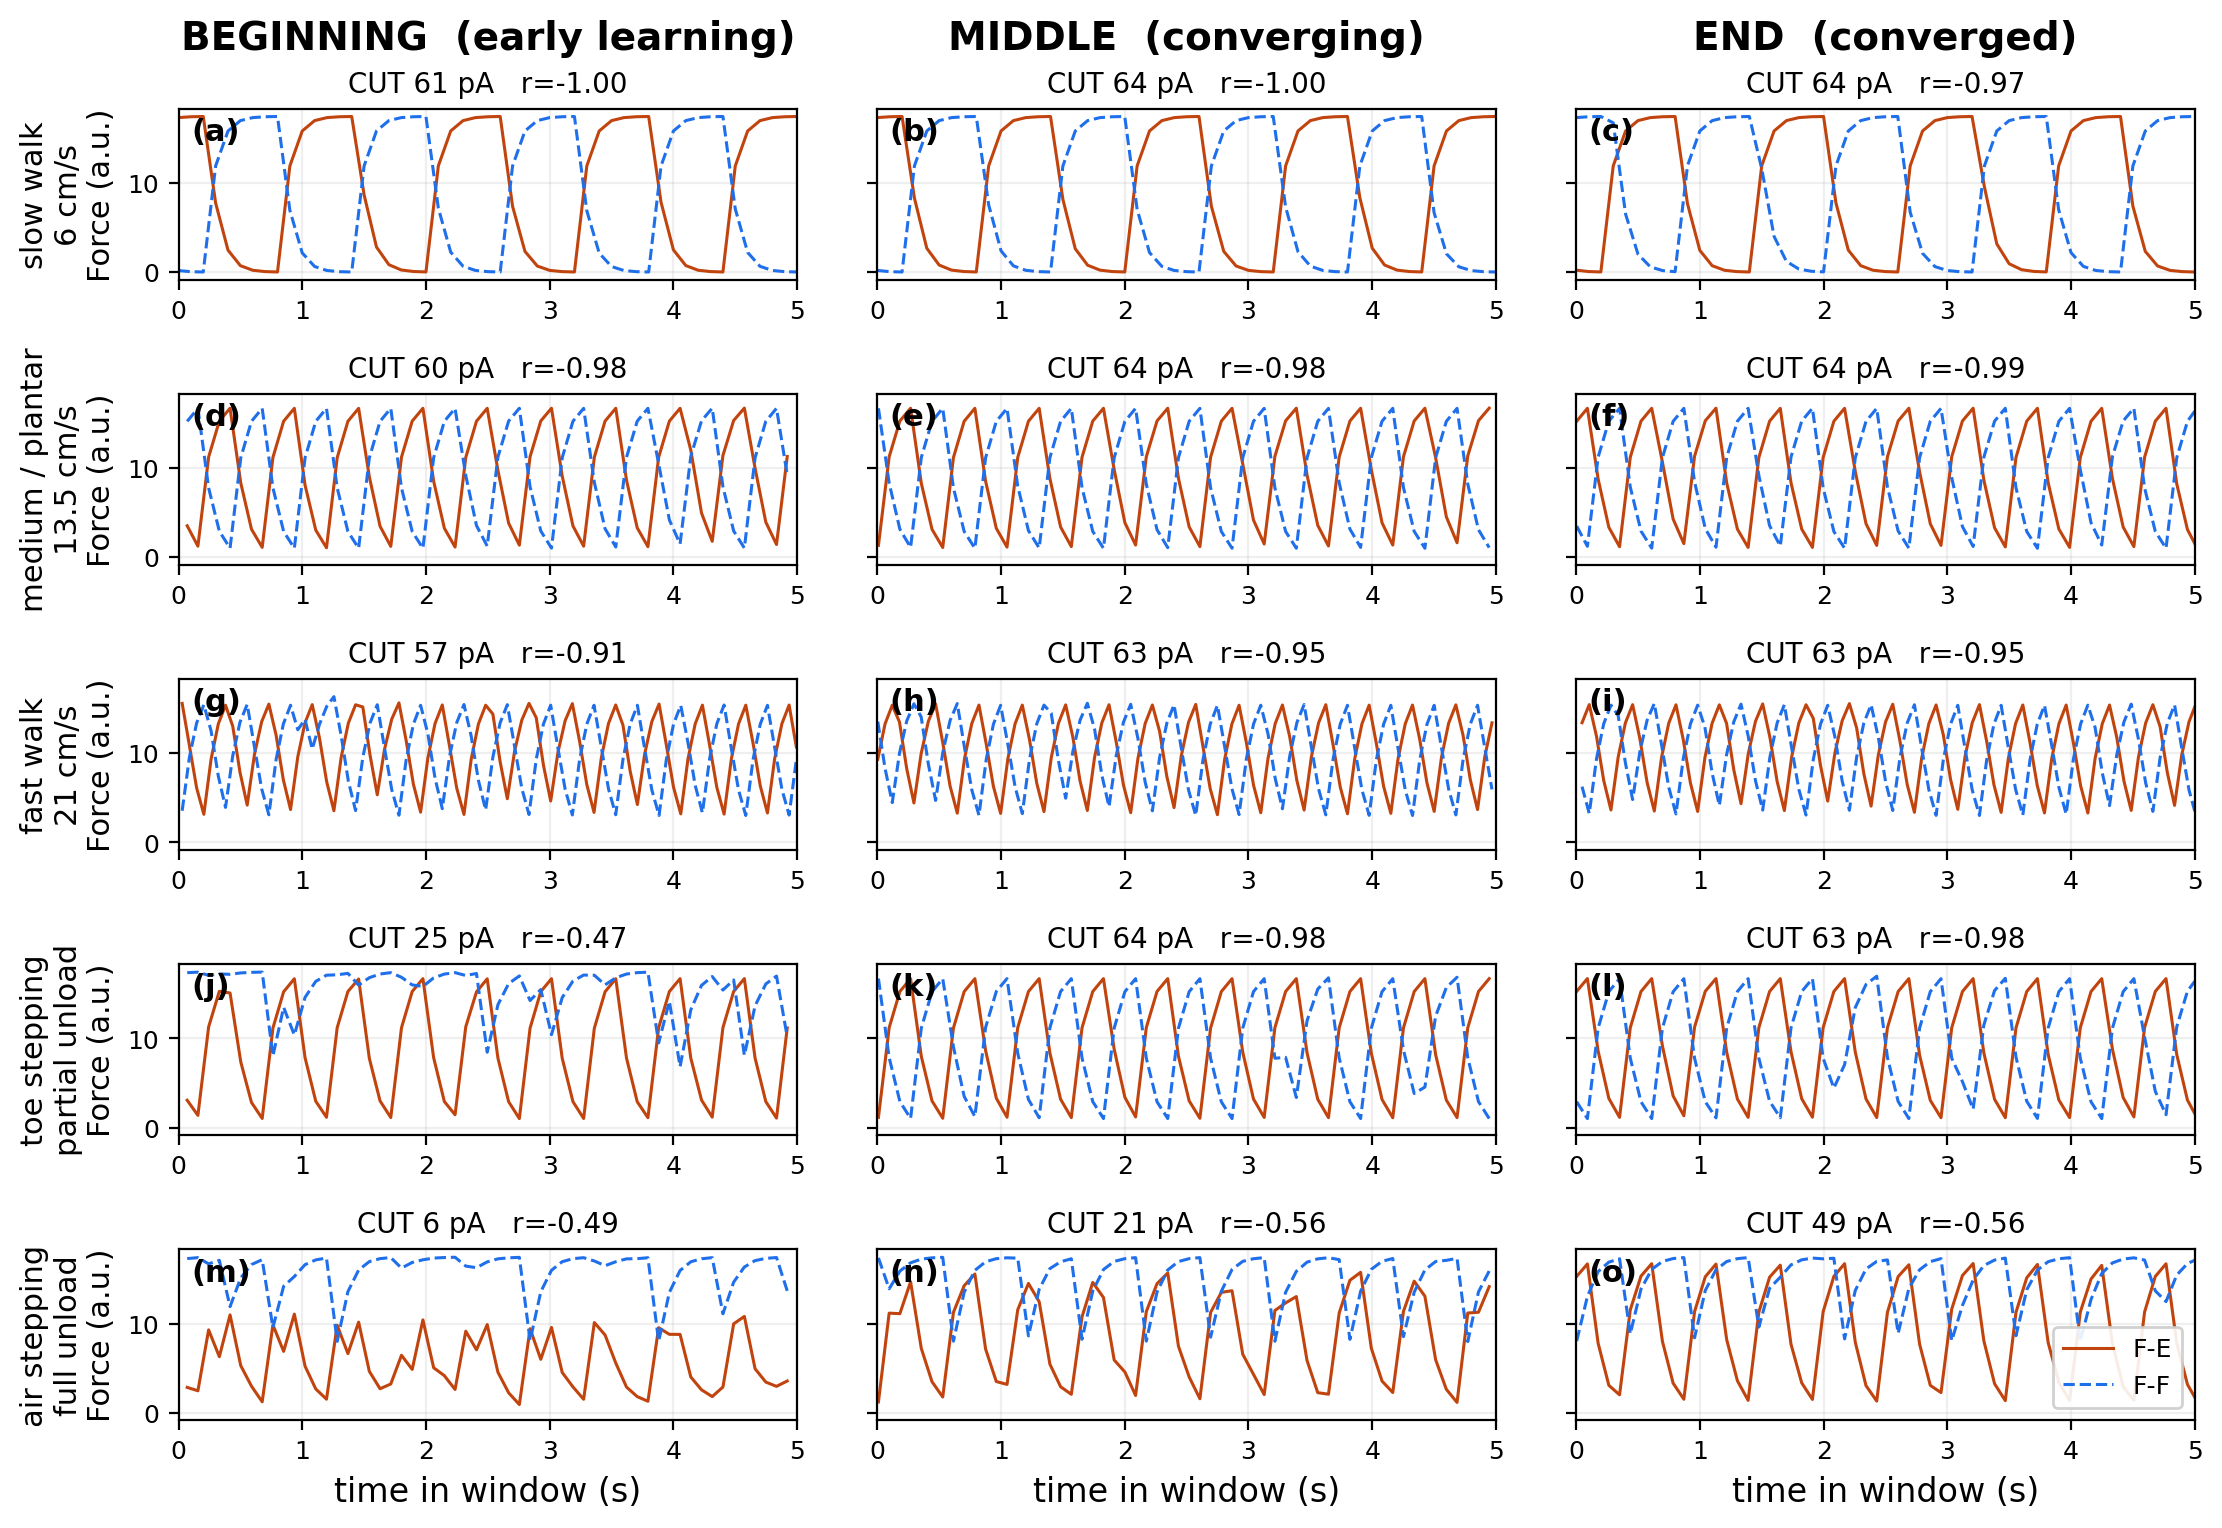
\includegraphics[width=0.9\textwidth]{fig_force_stages_lam1em3.png}
  \caption{\textbf{Force at three learning stages, five locomotion modes,
    $\lambda=10^{-3}$.} Same layout as Figure~\ref{fig:force_l2}.}
  \label{fig:force_l3}
\end{figure}

\begin{figure}[t]
  \centering
  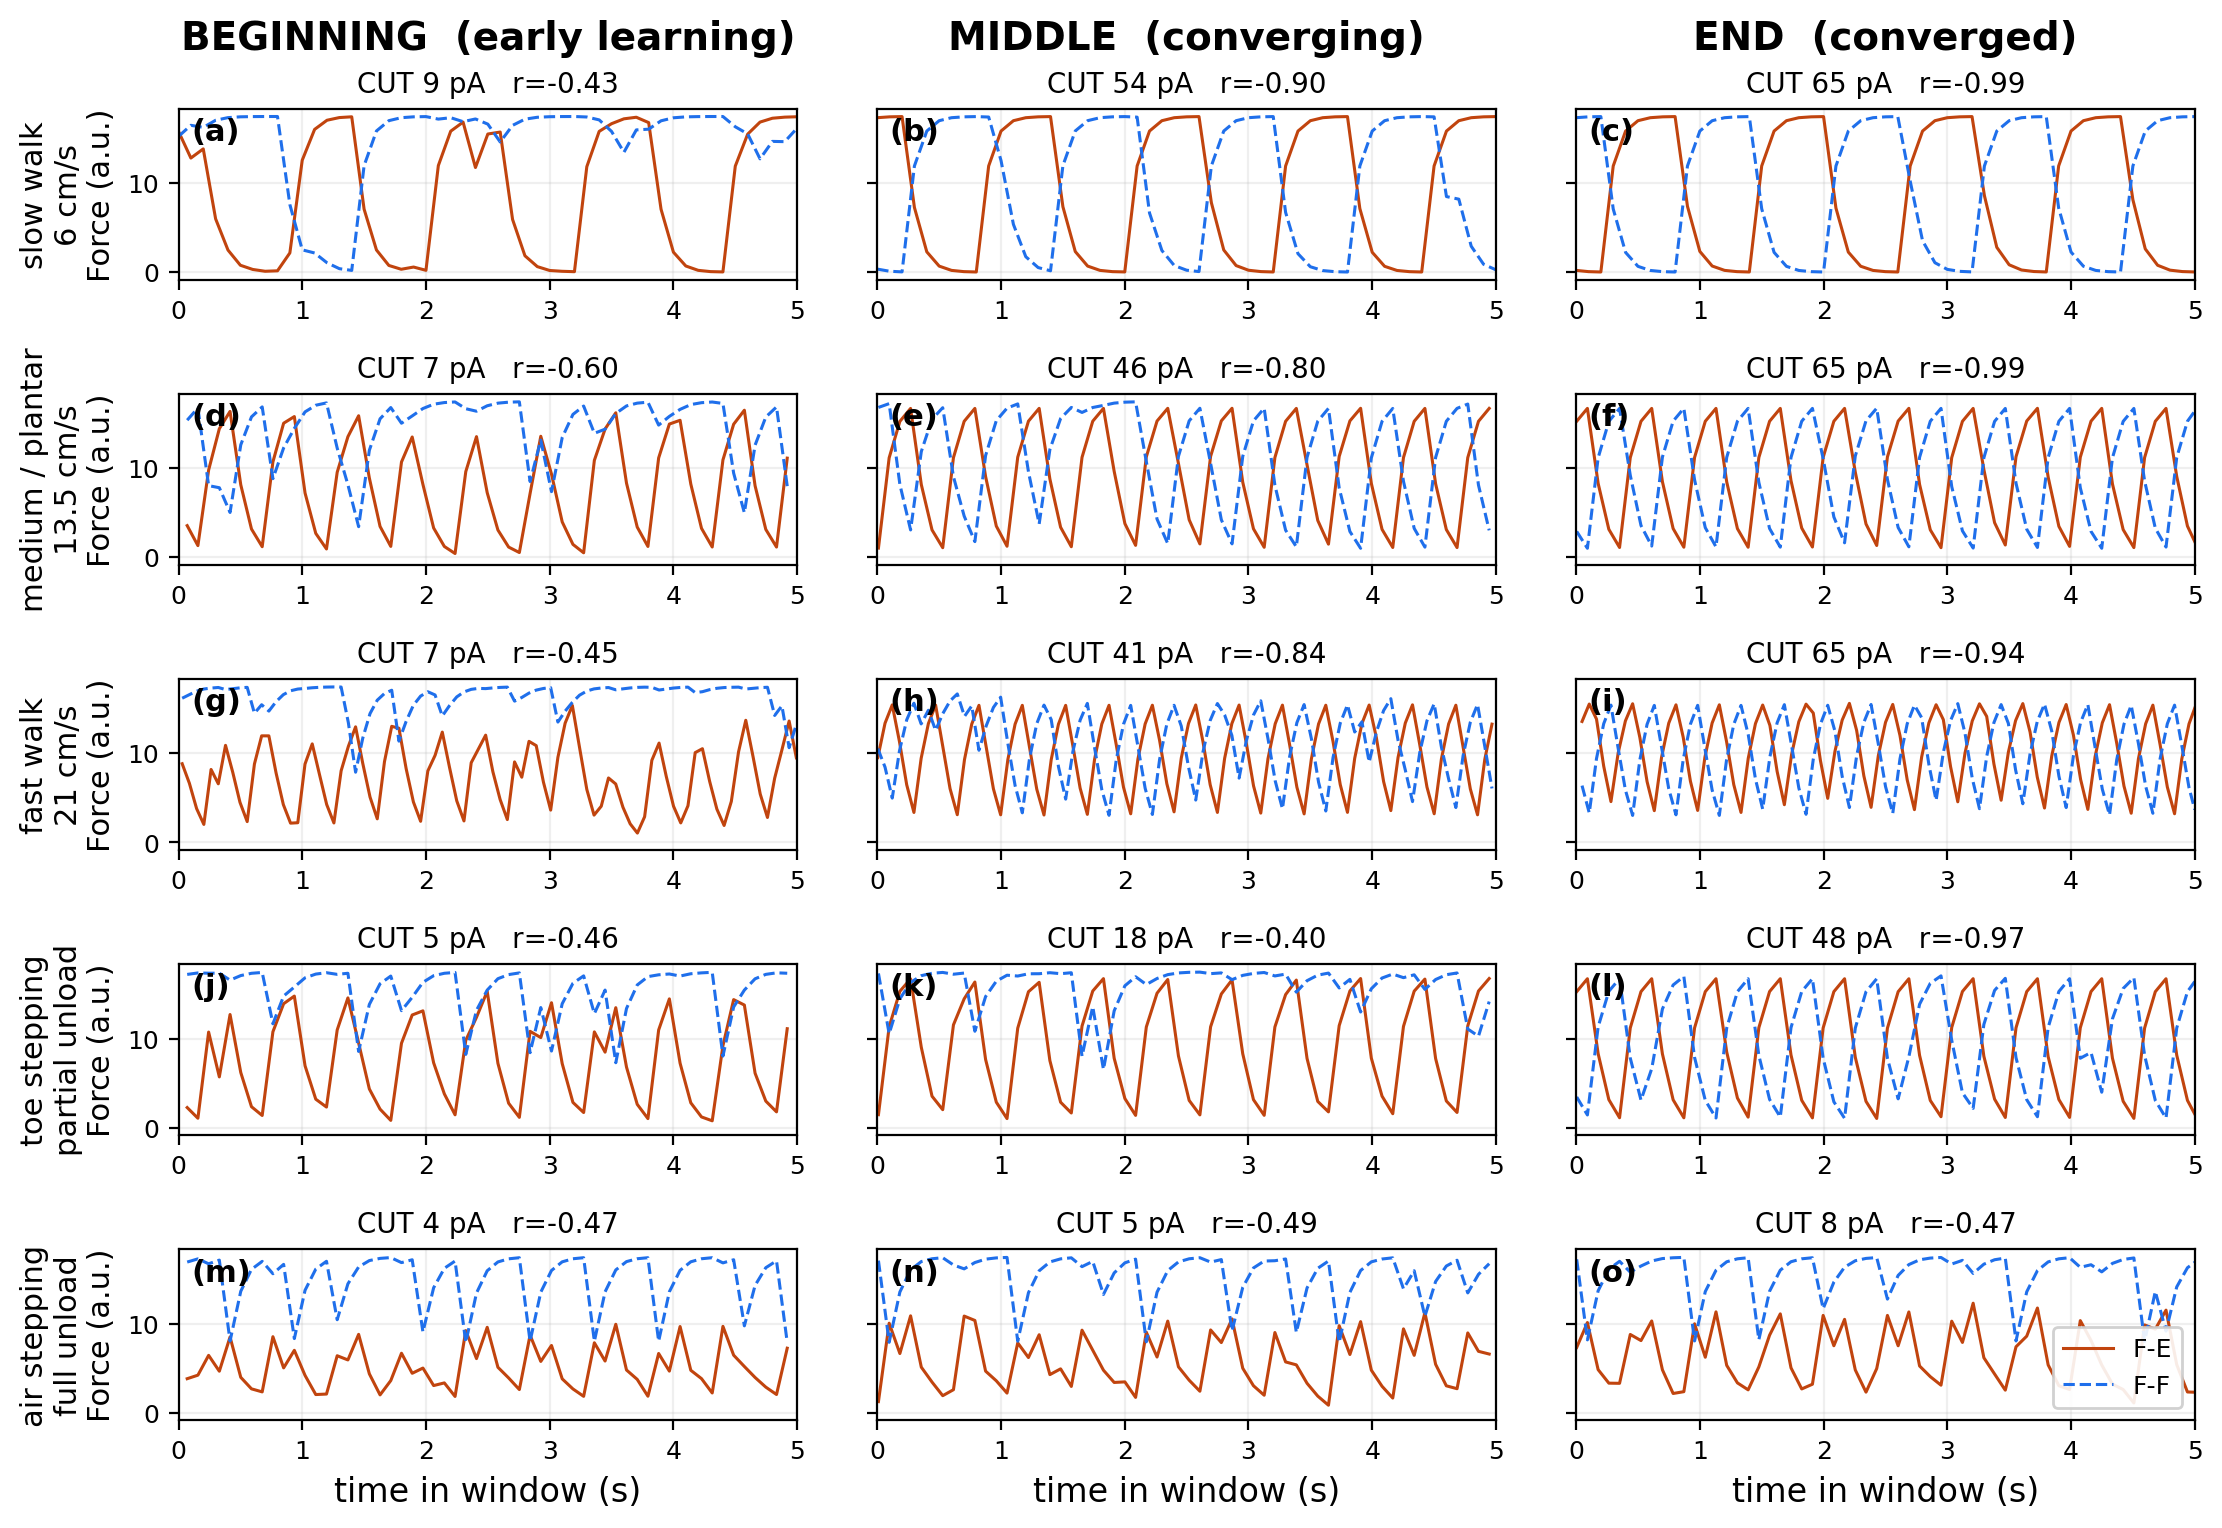
\includegraphics[width=0.9\textwidth]{fig_force_stages_lam1em4.png}
  \caption{\textbf{Force at three learning stages, five locomotion modes,
    $\lambda=10^{-4}$.} Same layout as Figure~\ref{fig:force_l3}. At this
    intermediate rate the three stages are most distinct, spanning the full
    $120$\,s convergence.}
  \label{fig:force_l4}
\end{figure}

\begin{figure}[t]
  \centering
  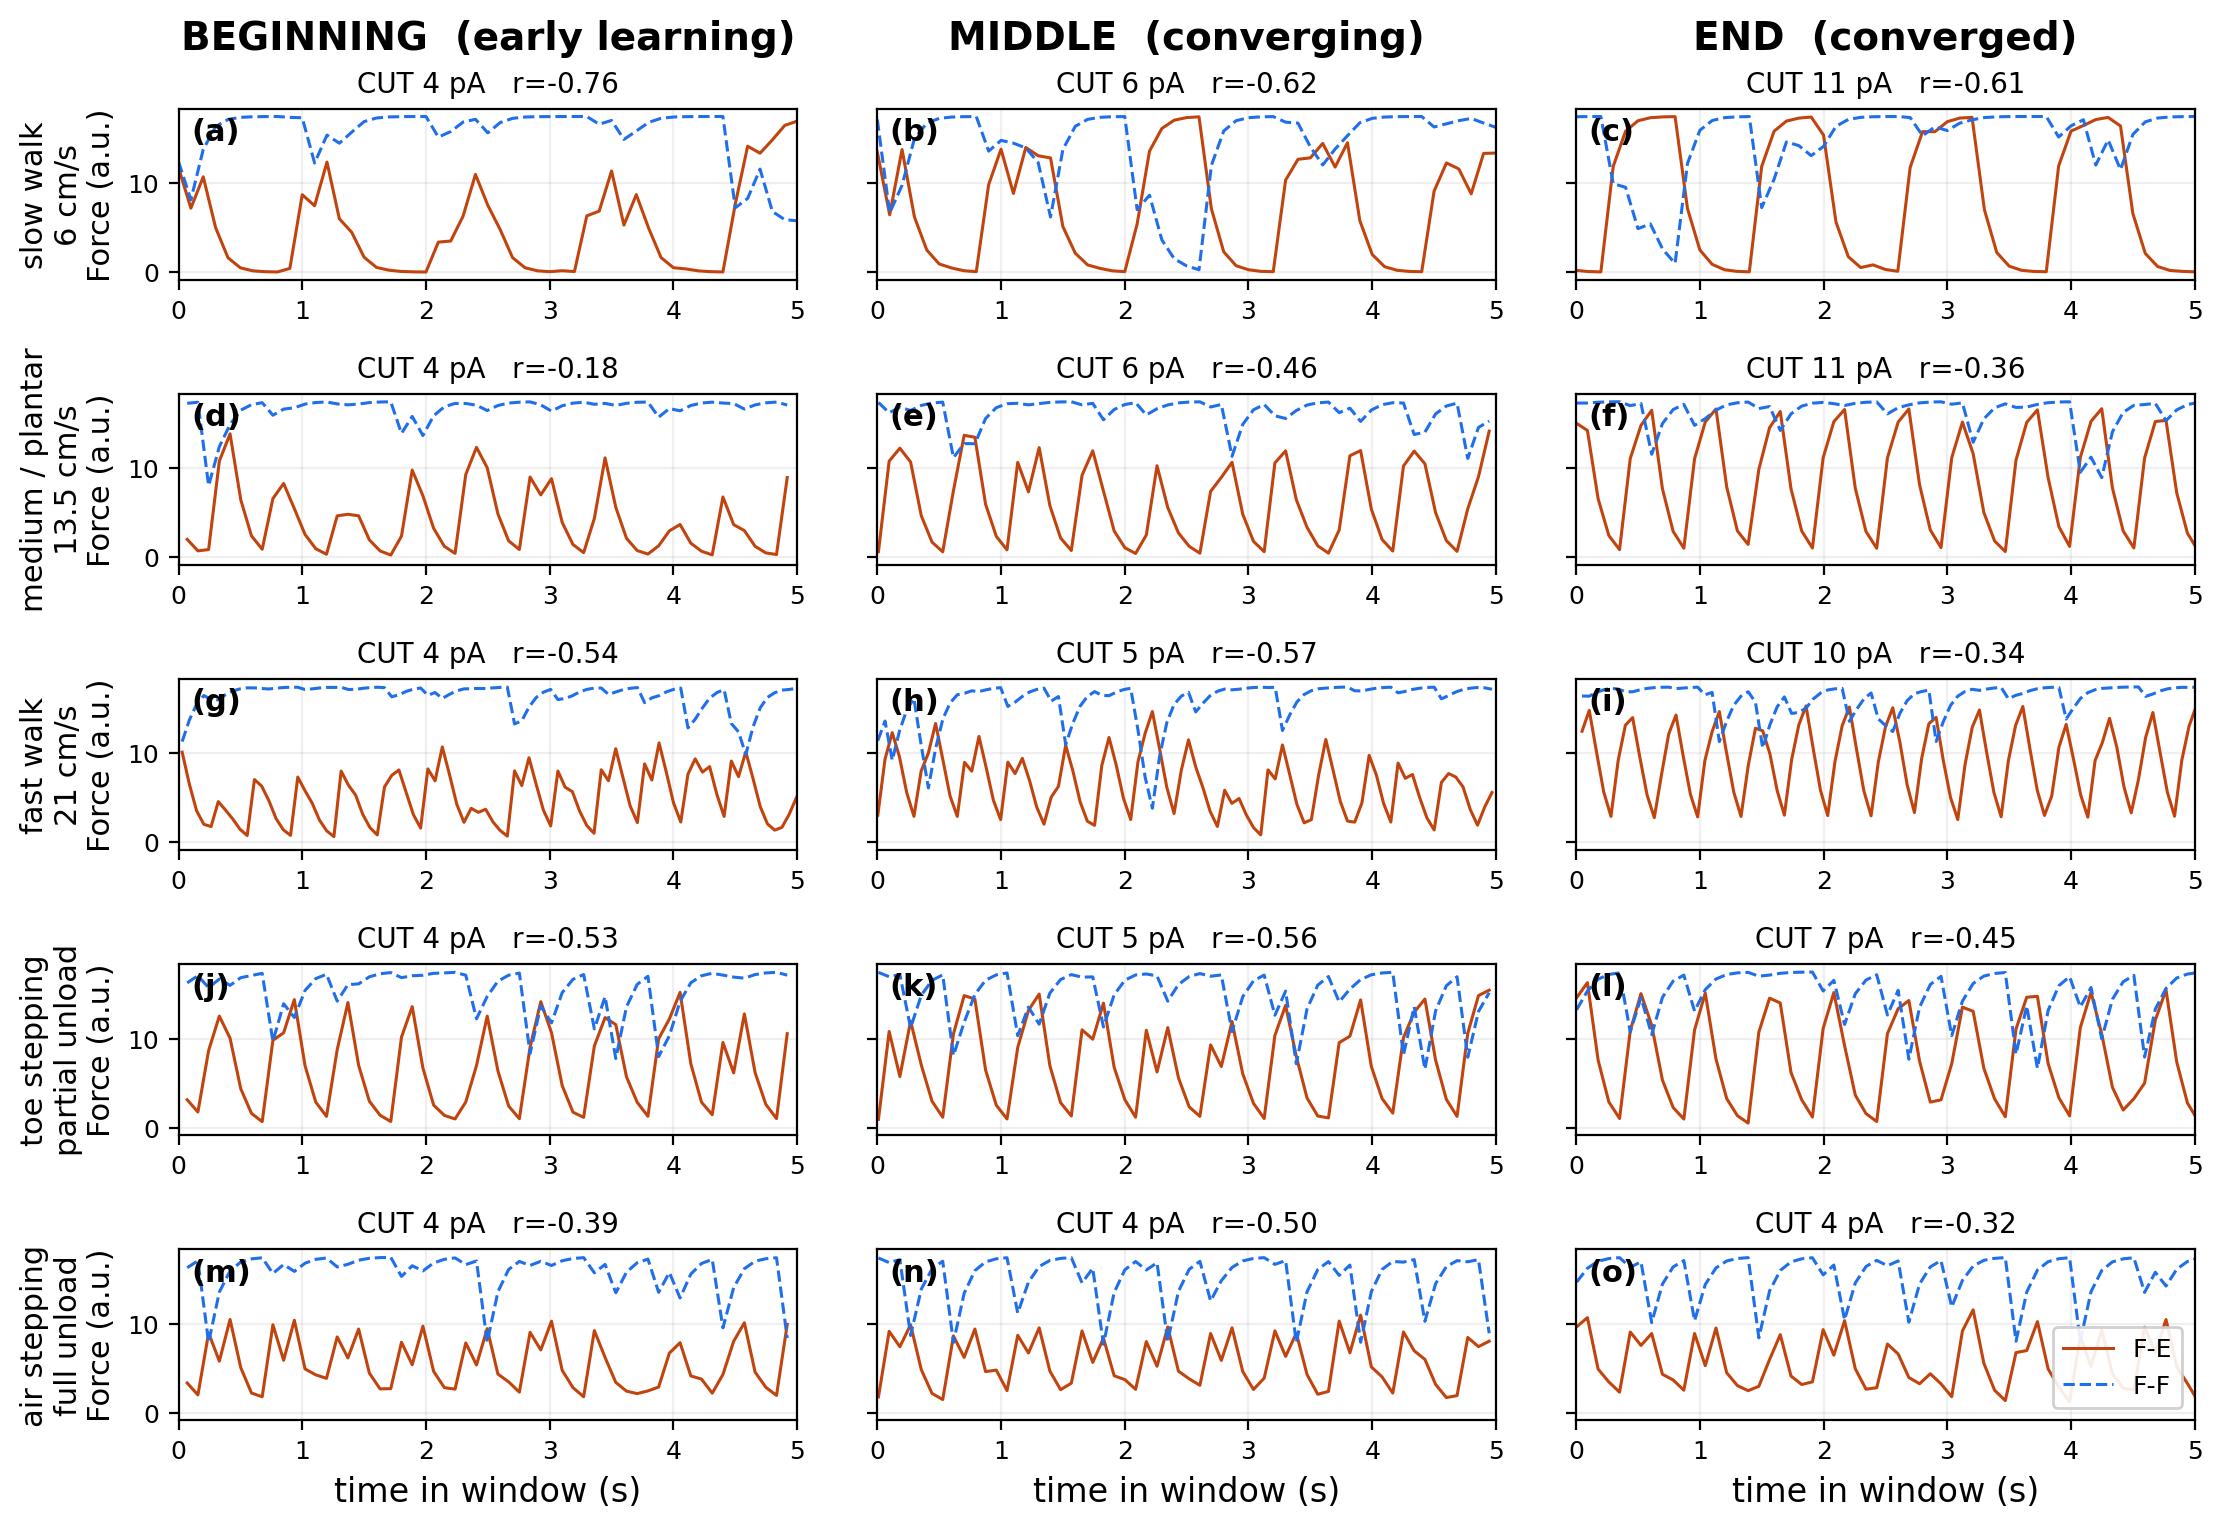
\includegraphics[width=0.9\textwidth]{fig_force_stages_lam1em5.png}
  \caption{\textbf{Force at three learning stages, five locomotion modes,
    $\lambda=10^{-5}$.} Same layout as Figure~\ref{fig:force_l2}. At this slow
    rate the descending weight barely develops within the run, so the gait stays
    under-developed across all three windows.}
  \label{fig:force_l5}
\end{figure}

\begin{figure}[t]
  \centering
  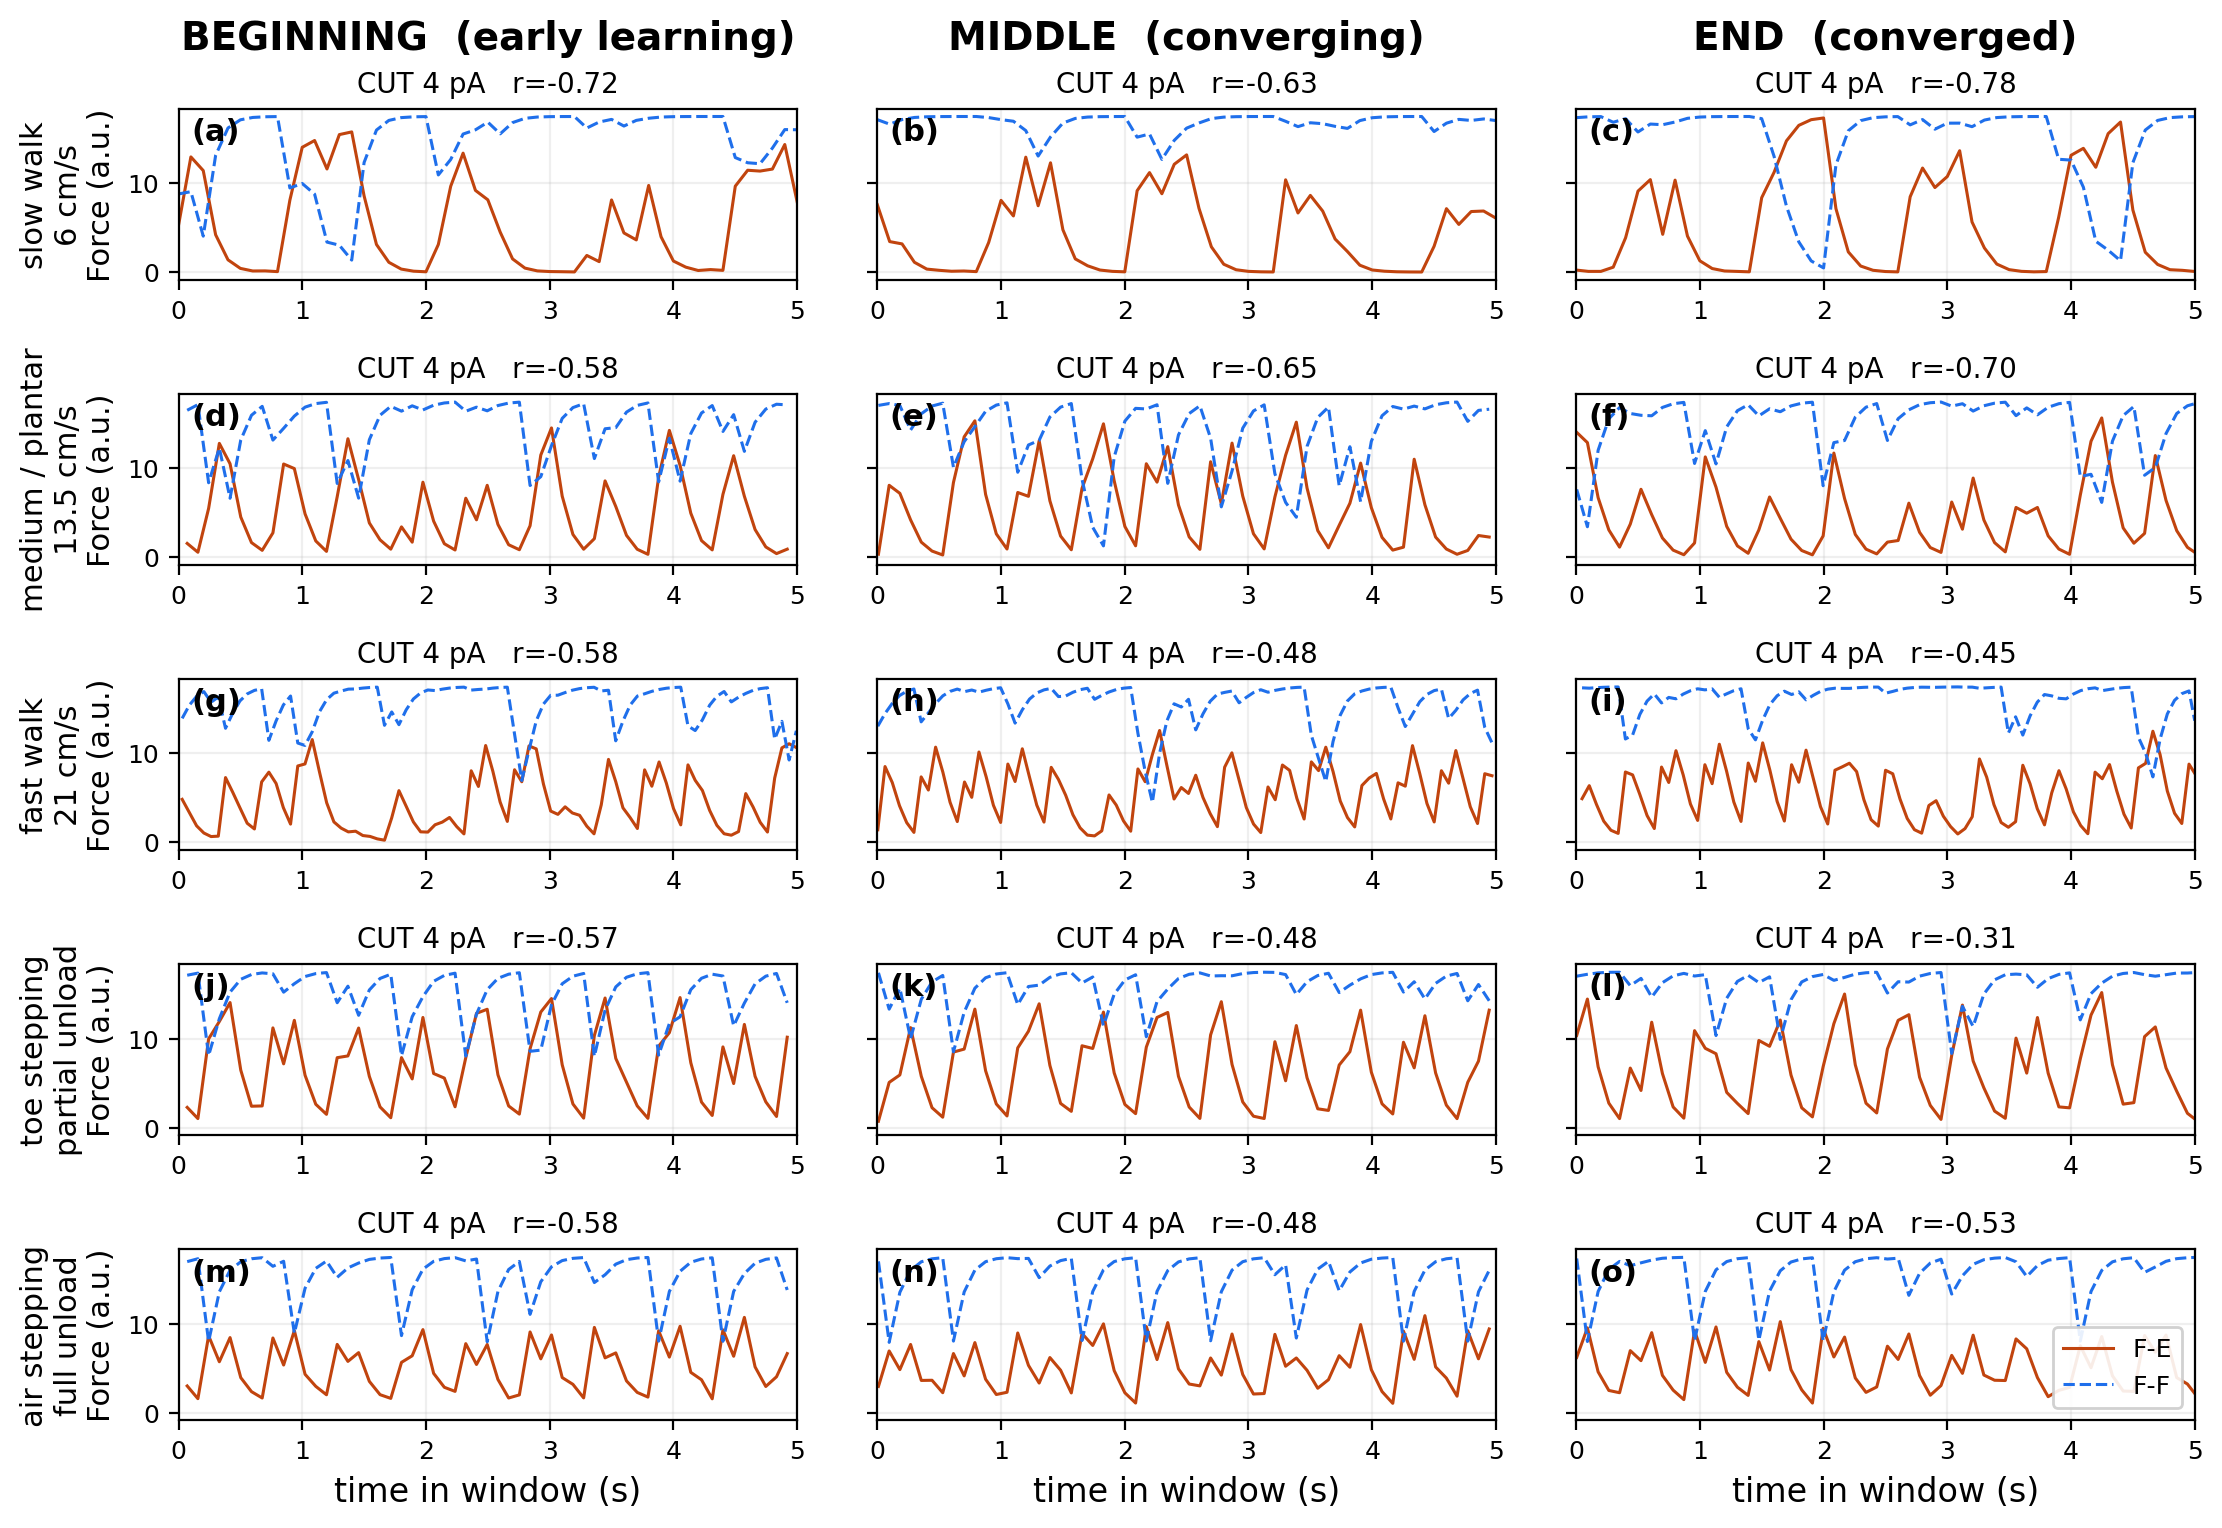
\includegraphics[width=0.9\textwidth]{fig_force_stages_lam1em6.png}
  \caption{\textbf{Force at three learning stages, five locomotion modes,
    $\lambda=10^{-6}$ (slowest rate).} Same layout as Figure~\ref{fig:force_l2};
    the descending weight remains near its initial value throughout, so
    counter-phase is carried almost entirely by the paced core.}
  \label{fig:force_l6}
\end{figure}

% =============================================================
\subsection{Network-level activity across the locomotion modes}\label{sec:results:network}

The muscle force is only the read-out of a whole network, so we next ask whether
the clean alternation is a property of the entire circuit.
Figures~\ref{fig:net_l2}--\ref{fig:net_l6} show the firing rates of all sixteen
recorded neuron pools --- for both legs, the rhythm generators (RG-E, RG-F), the
reciprocal-inhibition interneurons (InE, InF), the proprioceptive interneurons
(IaInt-E, IaInt-F) and the motor pools (M-E, M-F) --- one figure per learning
rate. In slow, medium and fast walk and in toe stepping, every extensor-side
pool fires in strict alternation with its flexor-side partner, the two legs stay
half a cycle apart (a $180^{\circ}$ offset, as in a real trot), and the
inhibitory interneurons alternate just as cleanly as the rhythm generators --- so
the alternation is built into the core circuit, not imposed only at the muscle.
The exception is air stepping (rightmost column): with the sensory feedback
withdrawn, the extensor-side pools (RG-E, InE, IaInt-E, M-E) fall nearly silent
while the flexor side, which bursts on its own intrinsic dynamics, keeps going
--- the network-level signature of the walking failure seen in the muscle forces.

\begin{figure}[t]
  \centering
  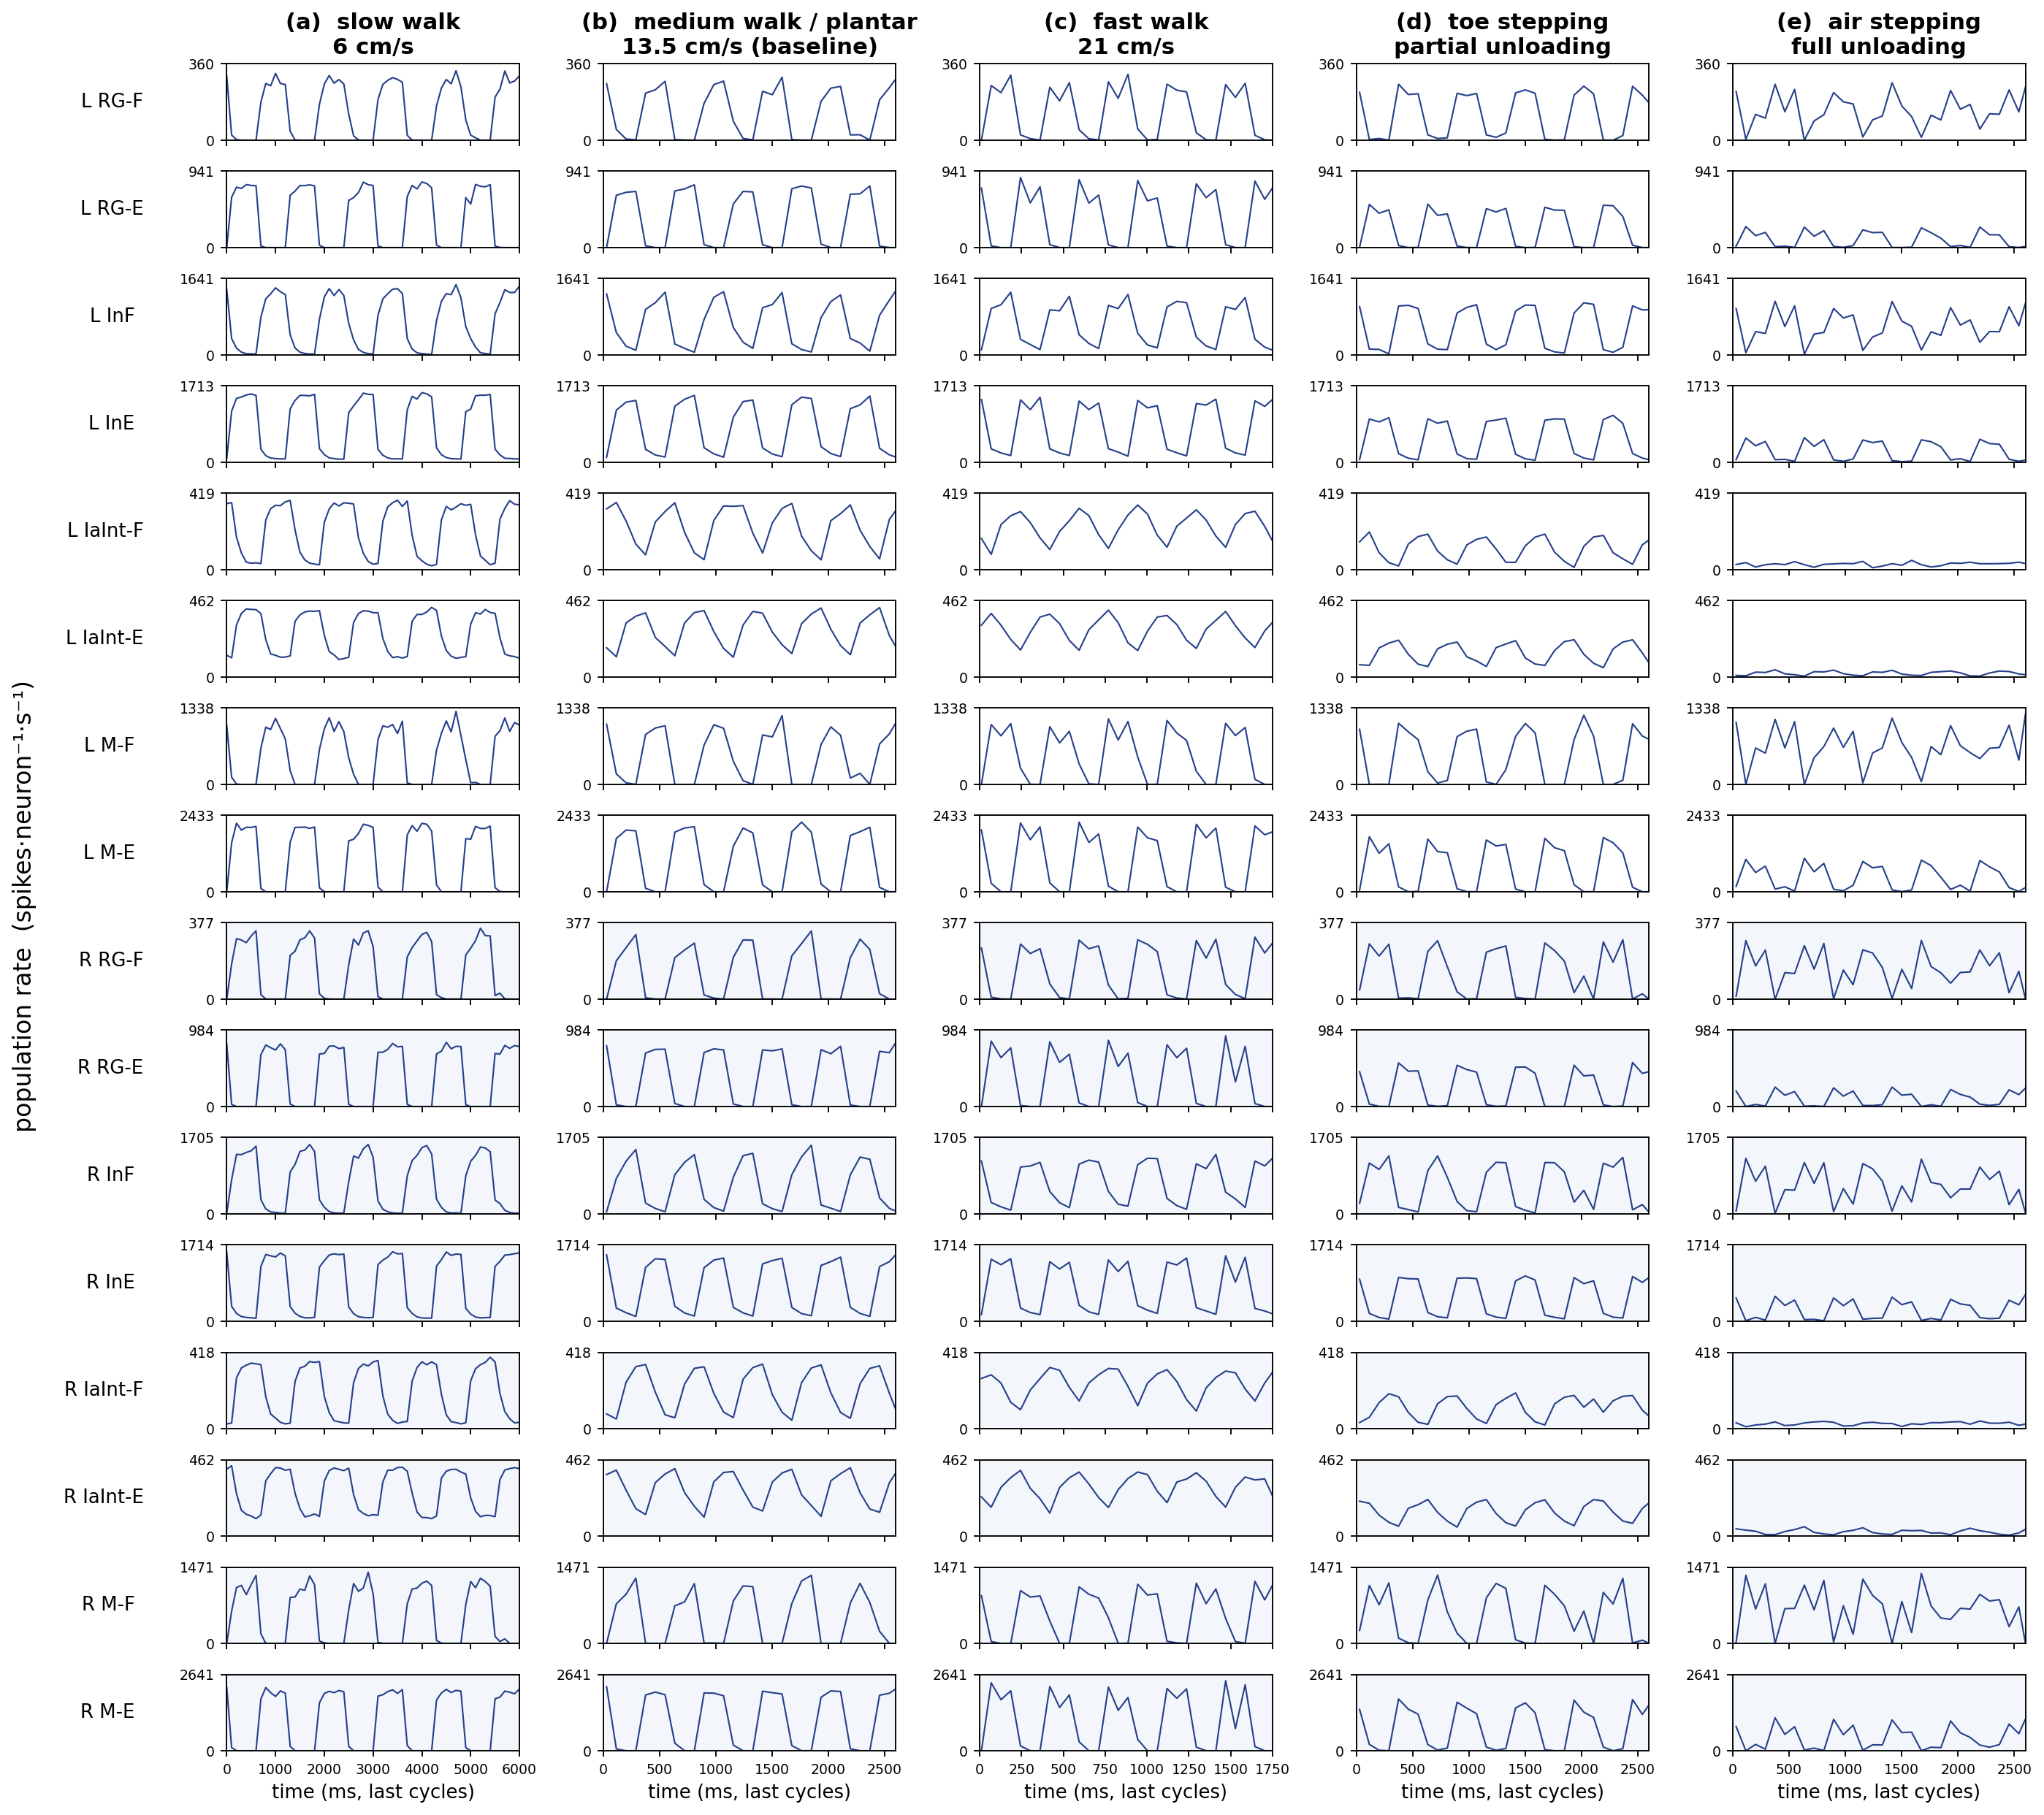
\includegraphics[width=0.95\textwidth]{fig_network_matrix_lam1em2.png}
  \caption{\textbf{Full-circuit population activity across the five locomotion
    modes, $\lambda=10^{-2}$ (fastest rate).} Rows: the sixteen recorded
    populations (both legs; right-leg rows tinted); columns (a)--(e): slow /
    medium=plantar=baseline / fast walk and toe / air stepping. Population rate
    (spikes$\cdot$neuron$^{-1}\cdot$s$^{-1}$) versus time (ms), last cycles.}
  \label{fig:net_l2}
\end{figure}

\begin{figure}[t]
  \centering
  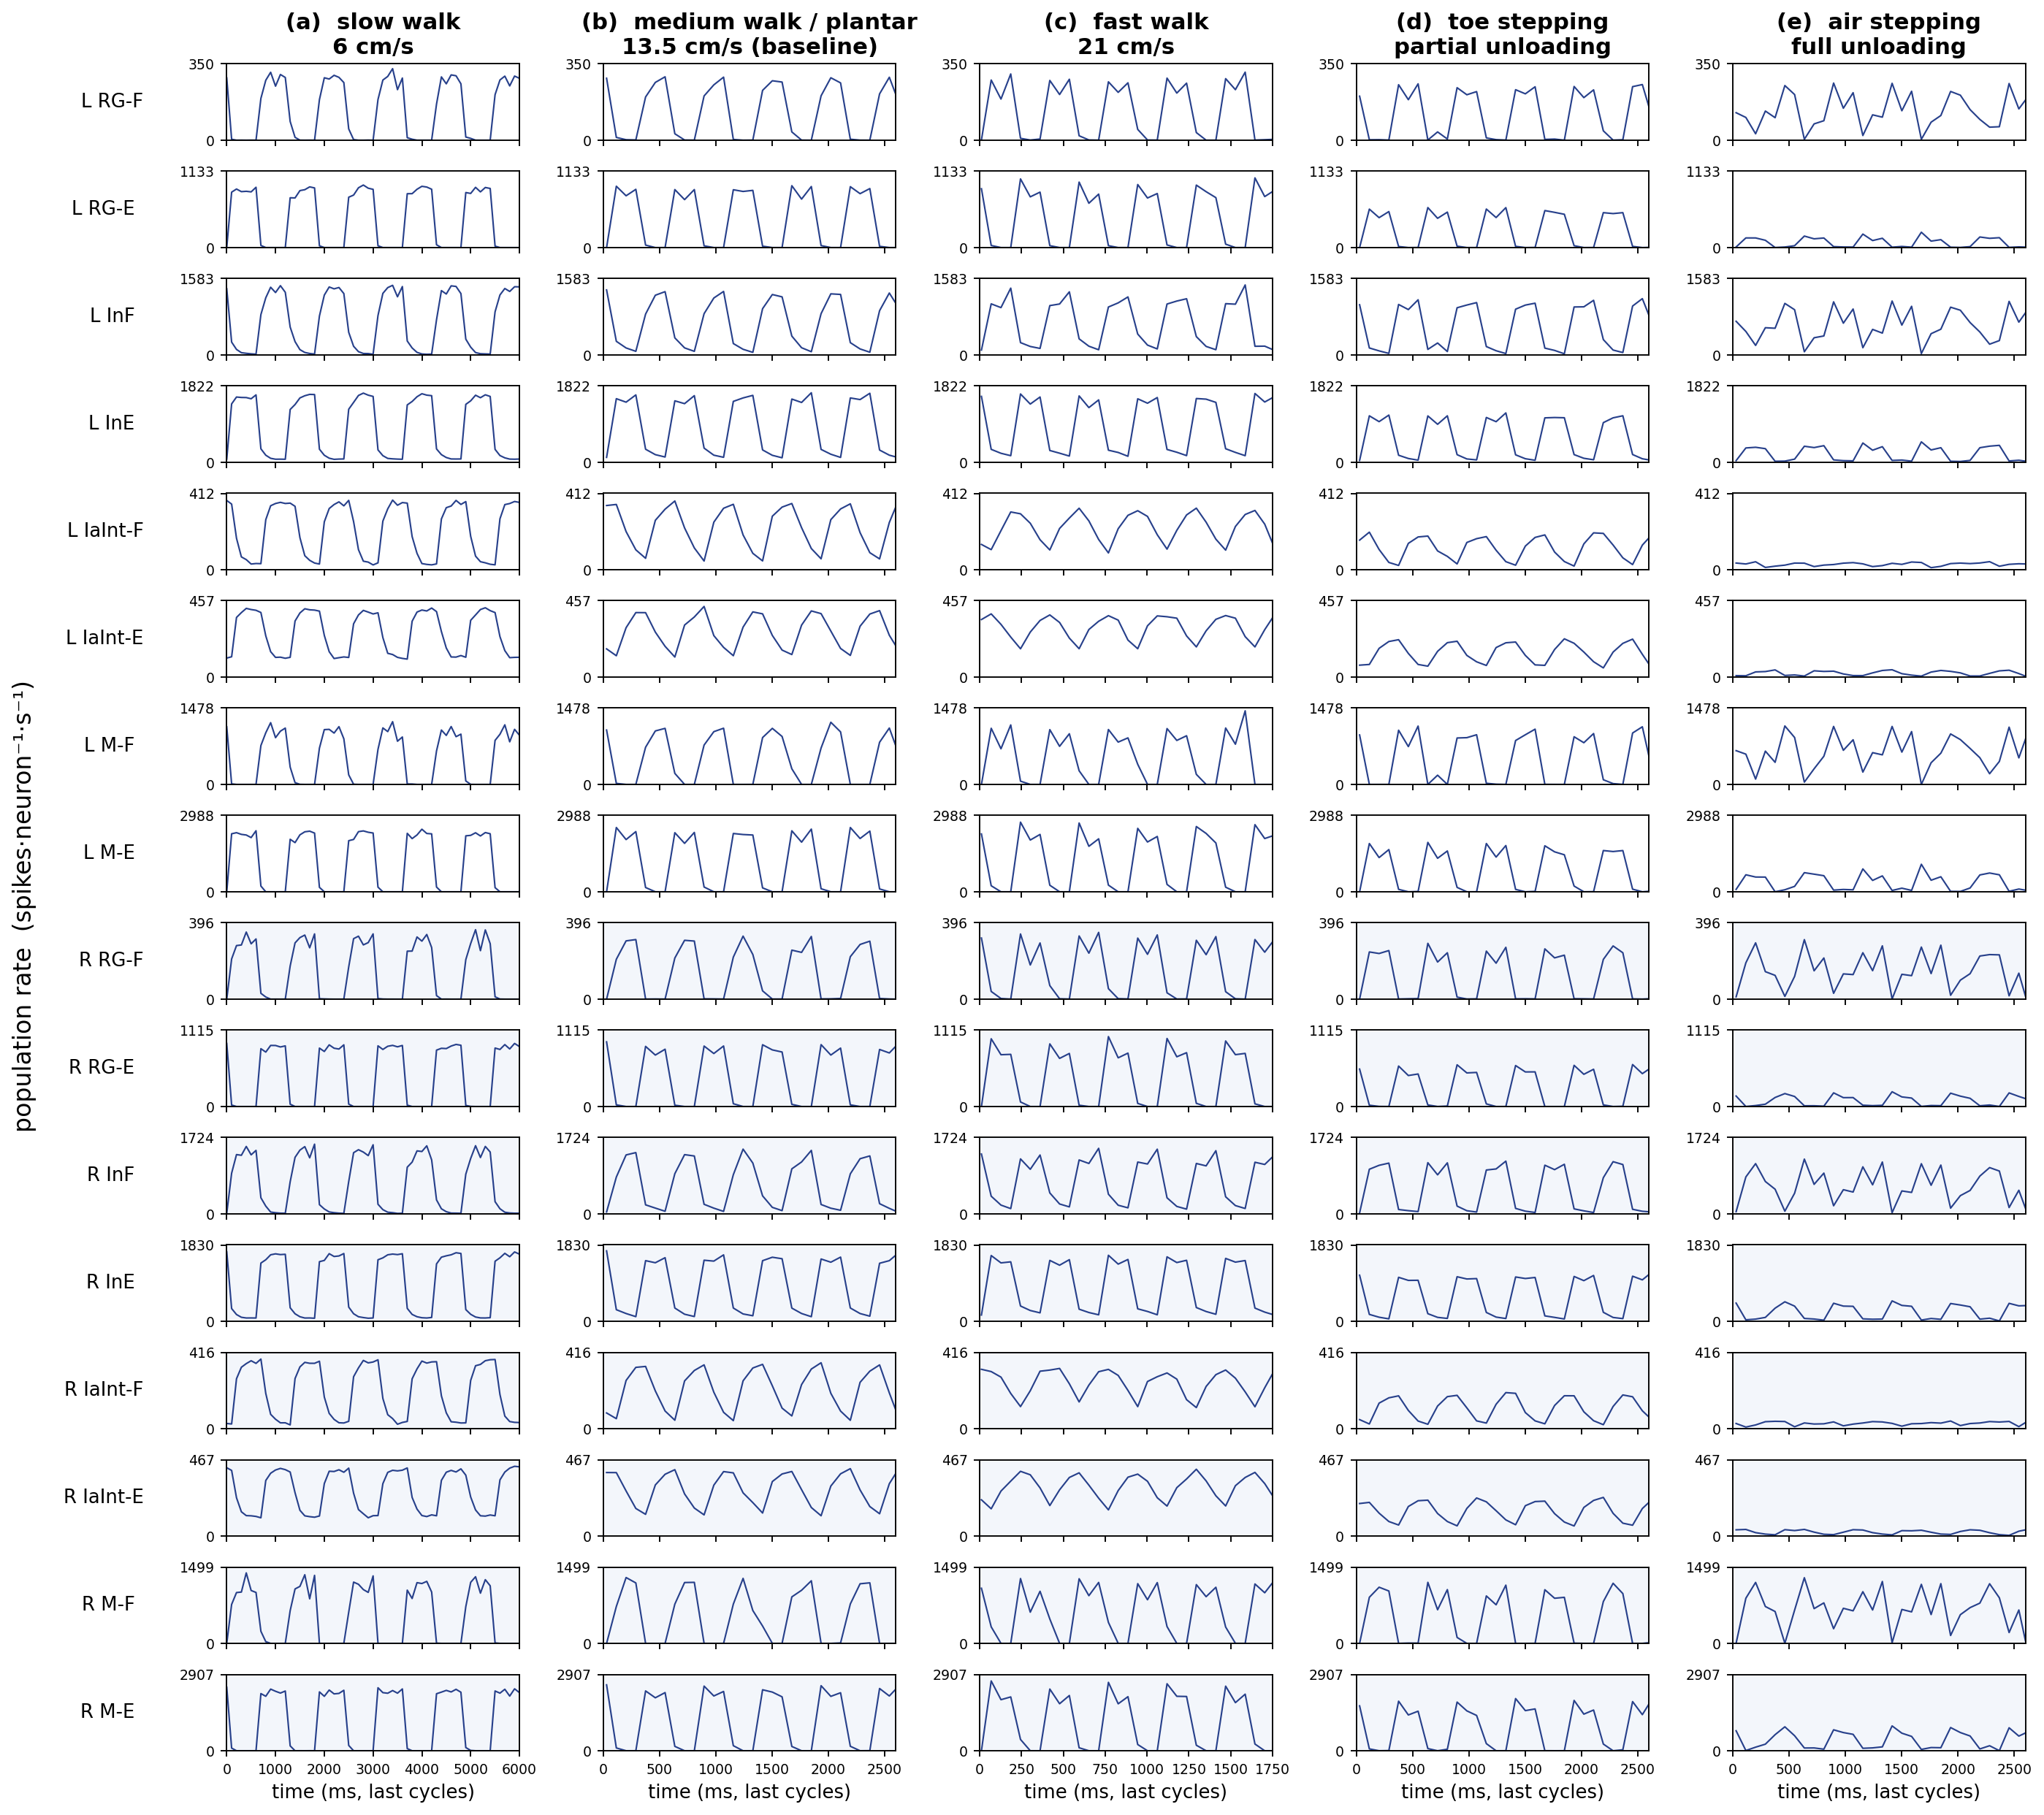
\includegraphics[width=0.95\textwidth]{fig_network_matrix_lam1em3.png}
  \caption{\textbf{Full-circuit population activity, $\lambda=10^{-3}$.} Same
    layout as Figure~\ref{fig:net_l2}.}
  \label{fig:net_l3}
\end{figure}

\begin{figure}[t]
  \centering
  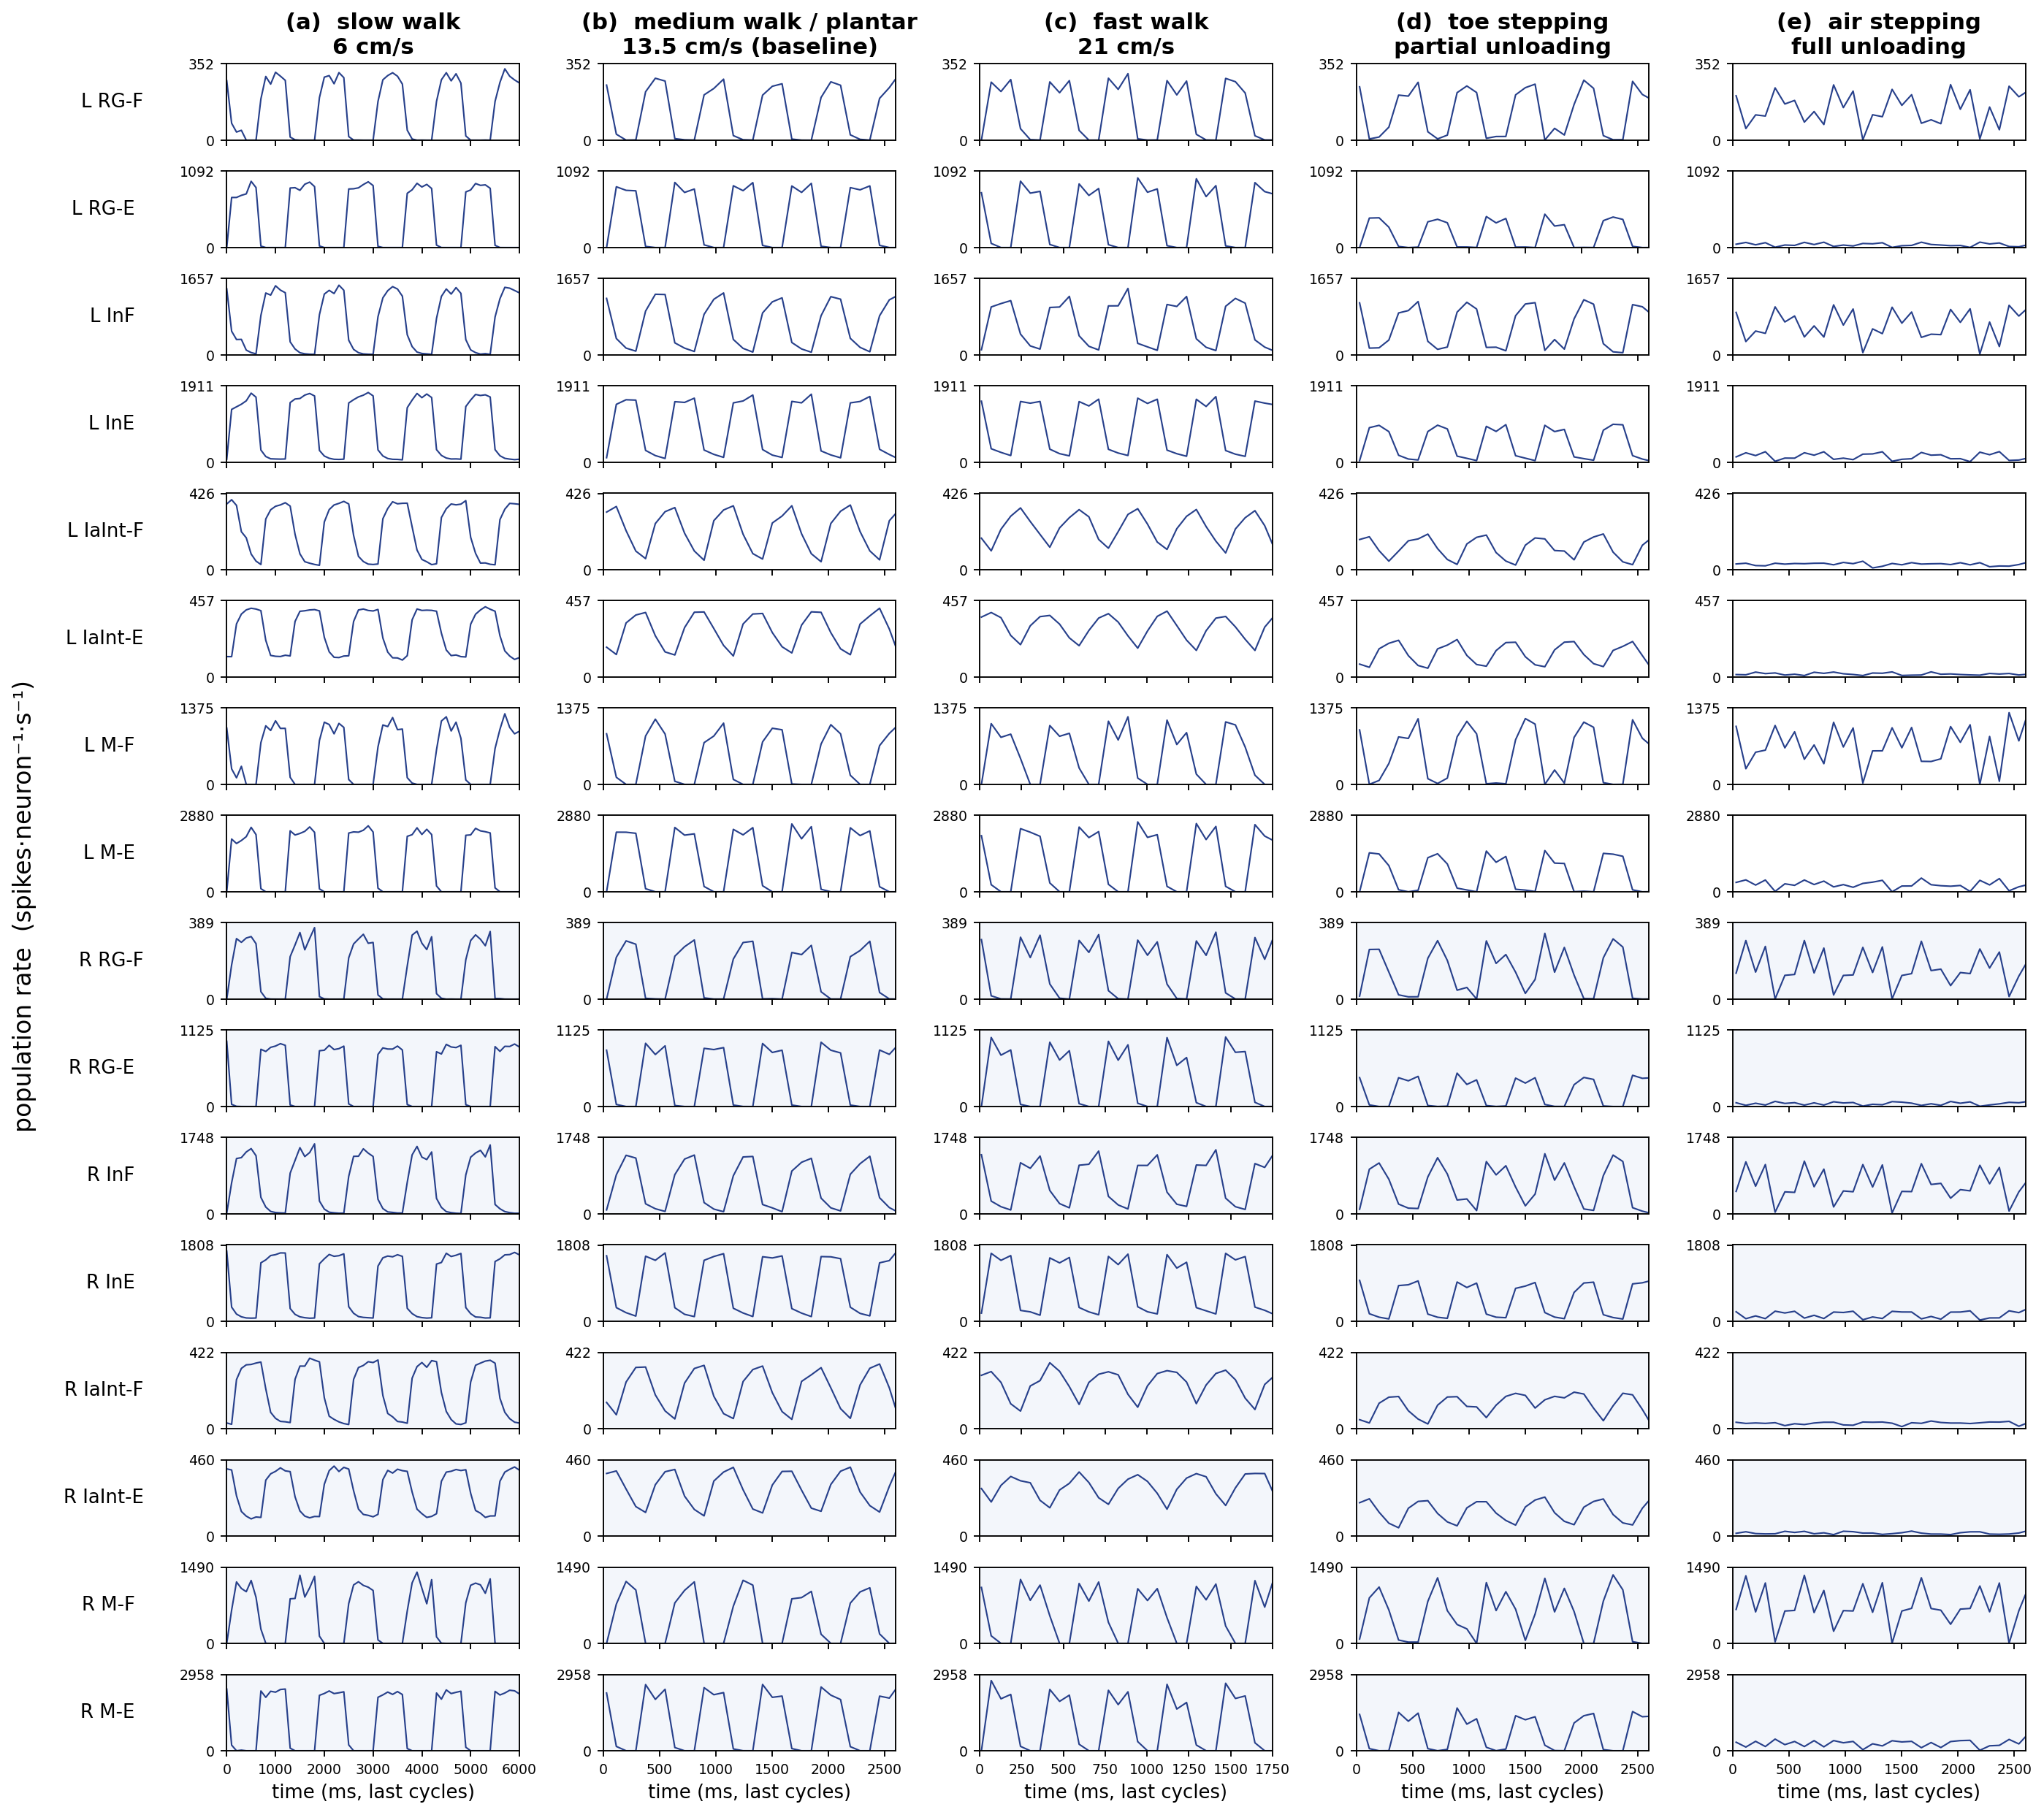
\includegraphics[width=0.95\textwidth]{fig_network_matrix_lam1em4.png}
  \caption{\textbf{Full-circuit population activity, $\lambda=10^{-4}$.} Same
    layout as Figure~\ref{fig:net_l3}.}
  \label{fig:net_l4}
\end{figure}

\begin{figure}[t]
  \centering
  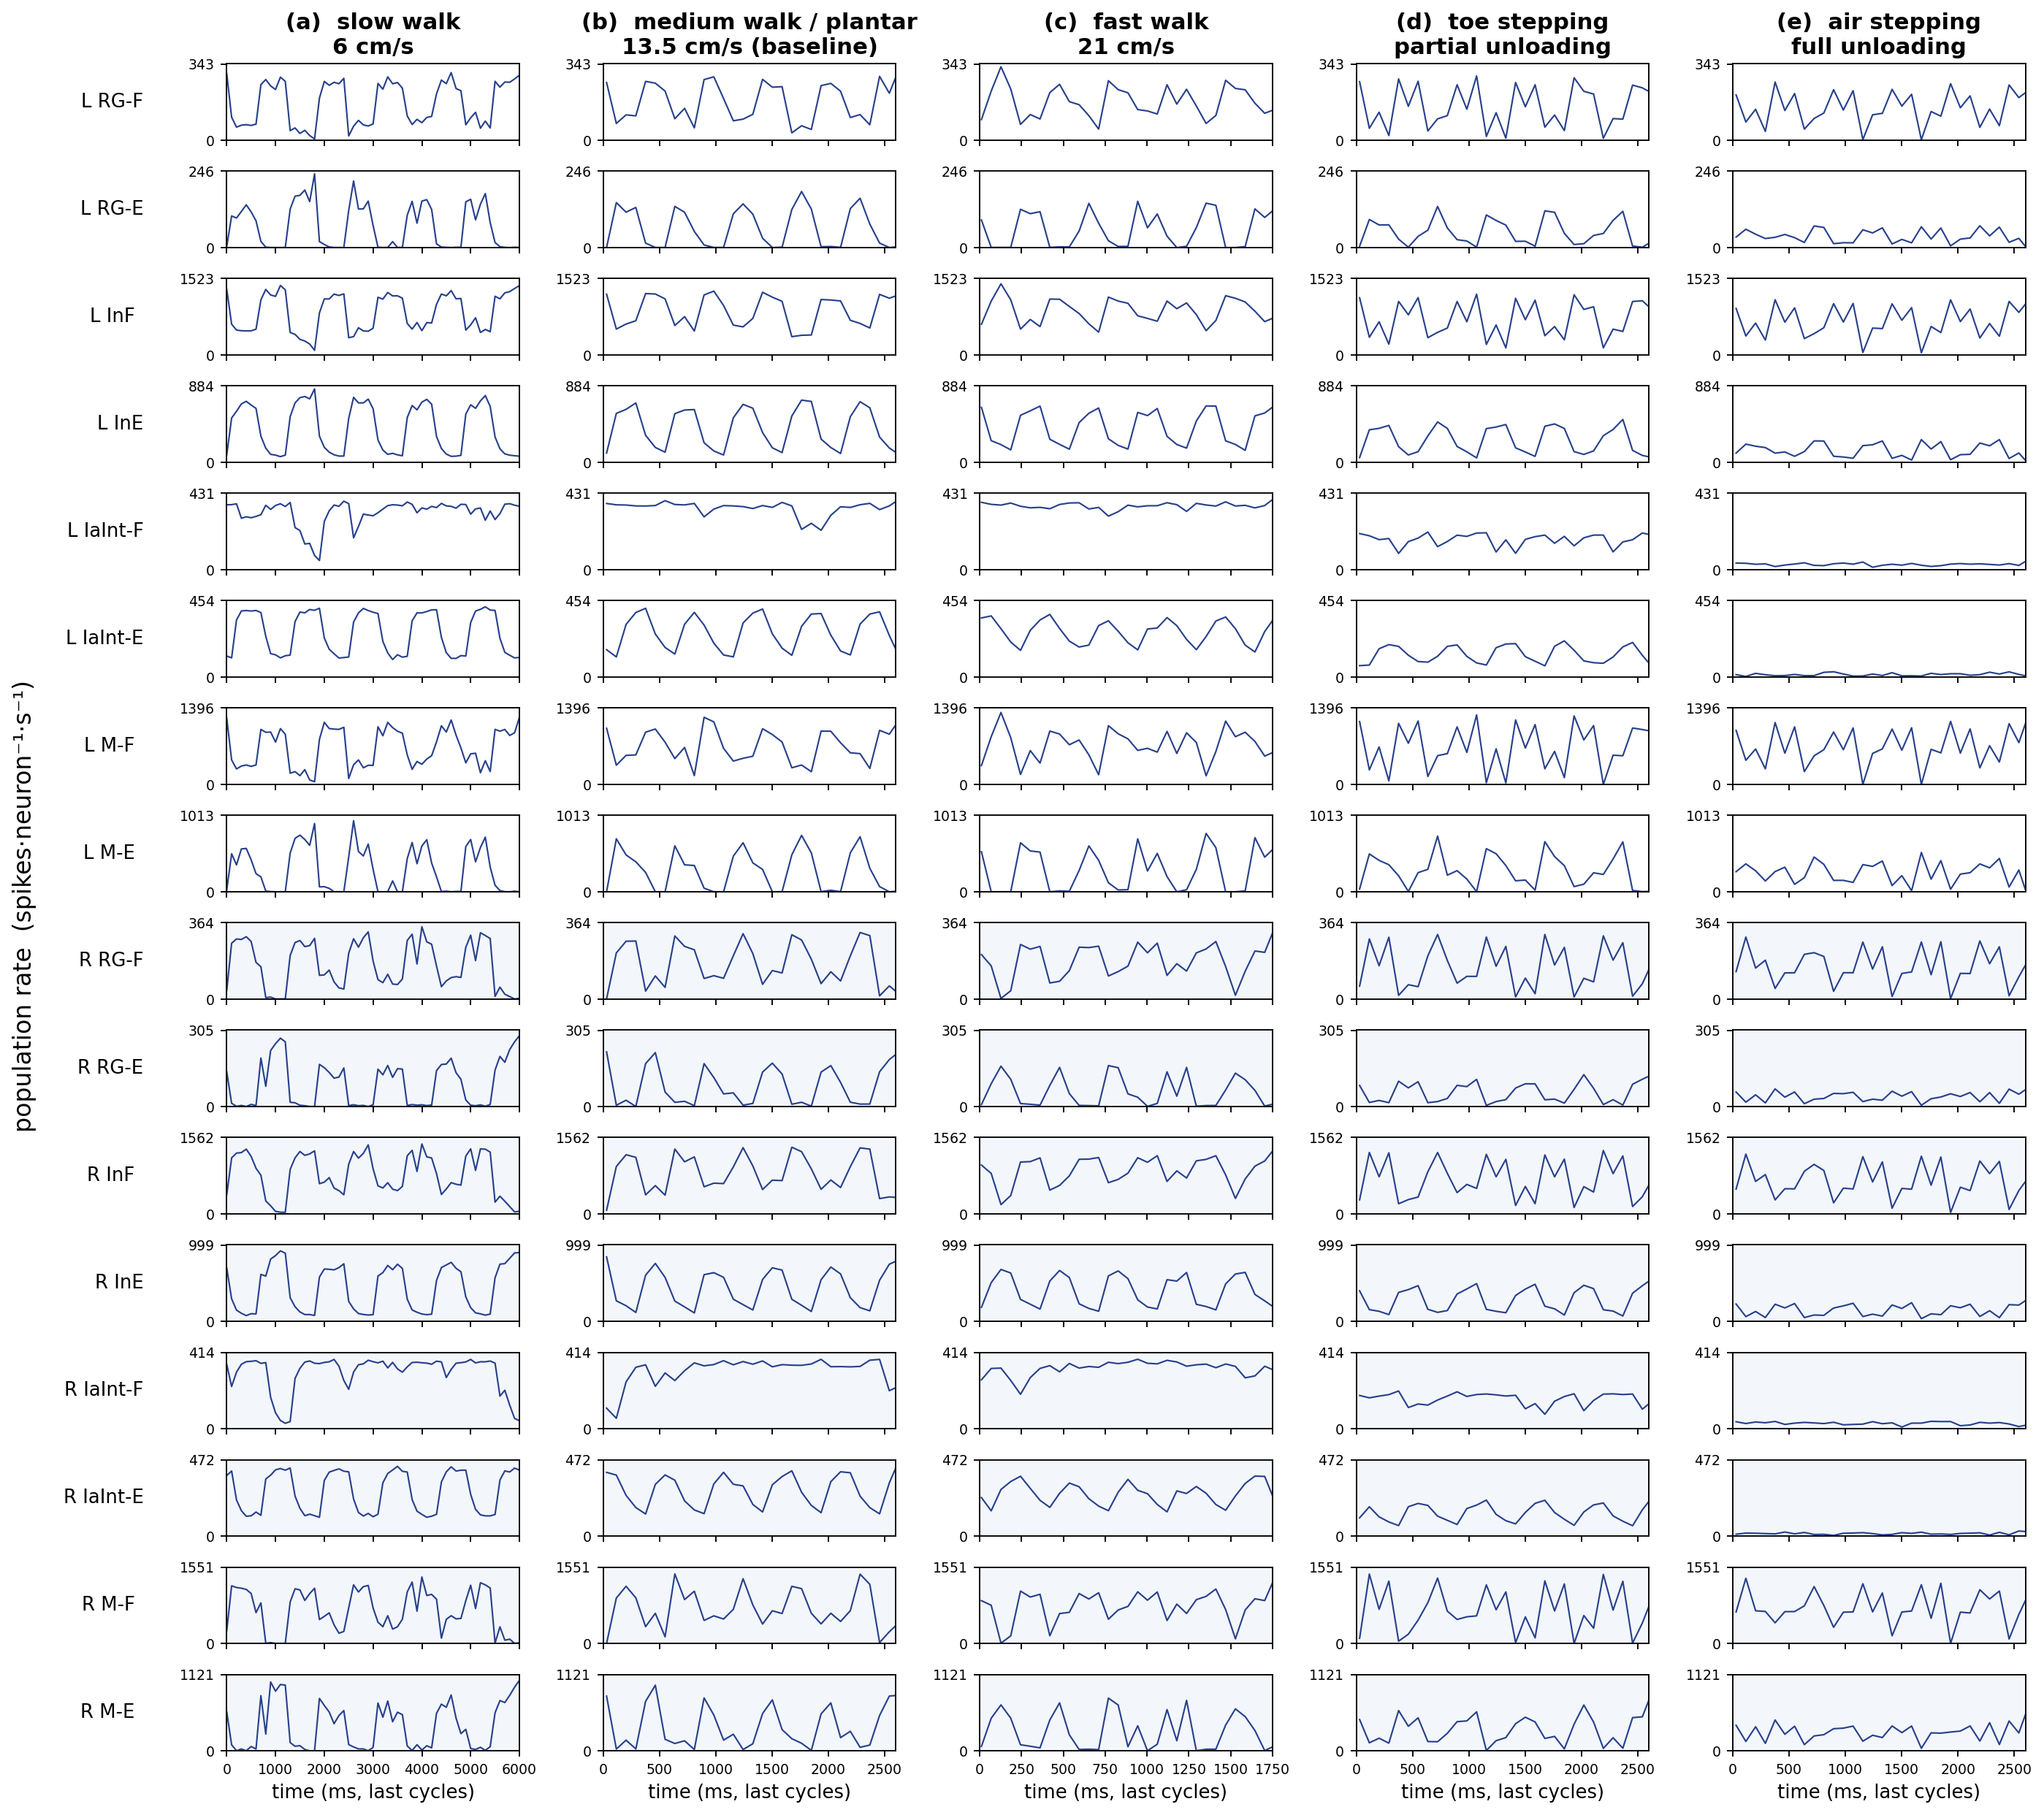
\includegraphics[width=0.95\textwidth]{fig_network_matrix_lam1em5.png}
  \caption{\textbf{Full-circuit population activity, $\lambda=10^{-5}$.} Same
    layout as Figure~\ref{fig:net_l2}. At this under-converged rate the
    counter-phase is weaker, most visibly at the higher cadences.}
  \label{fig:net_l5}
\end{figure}

\begin{figure}[t]
  \centering
  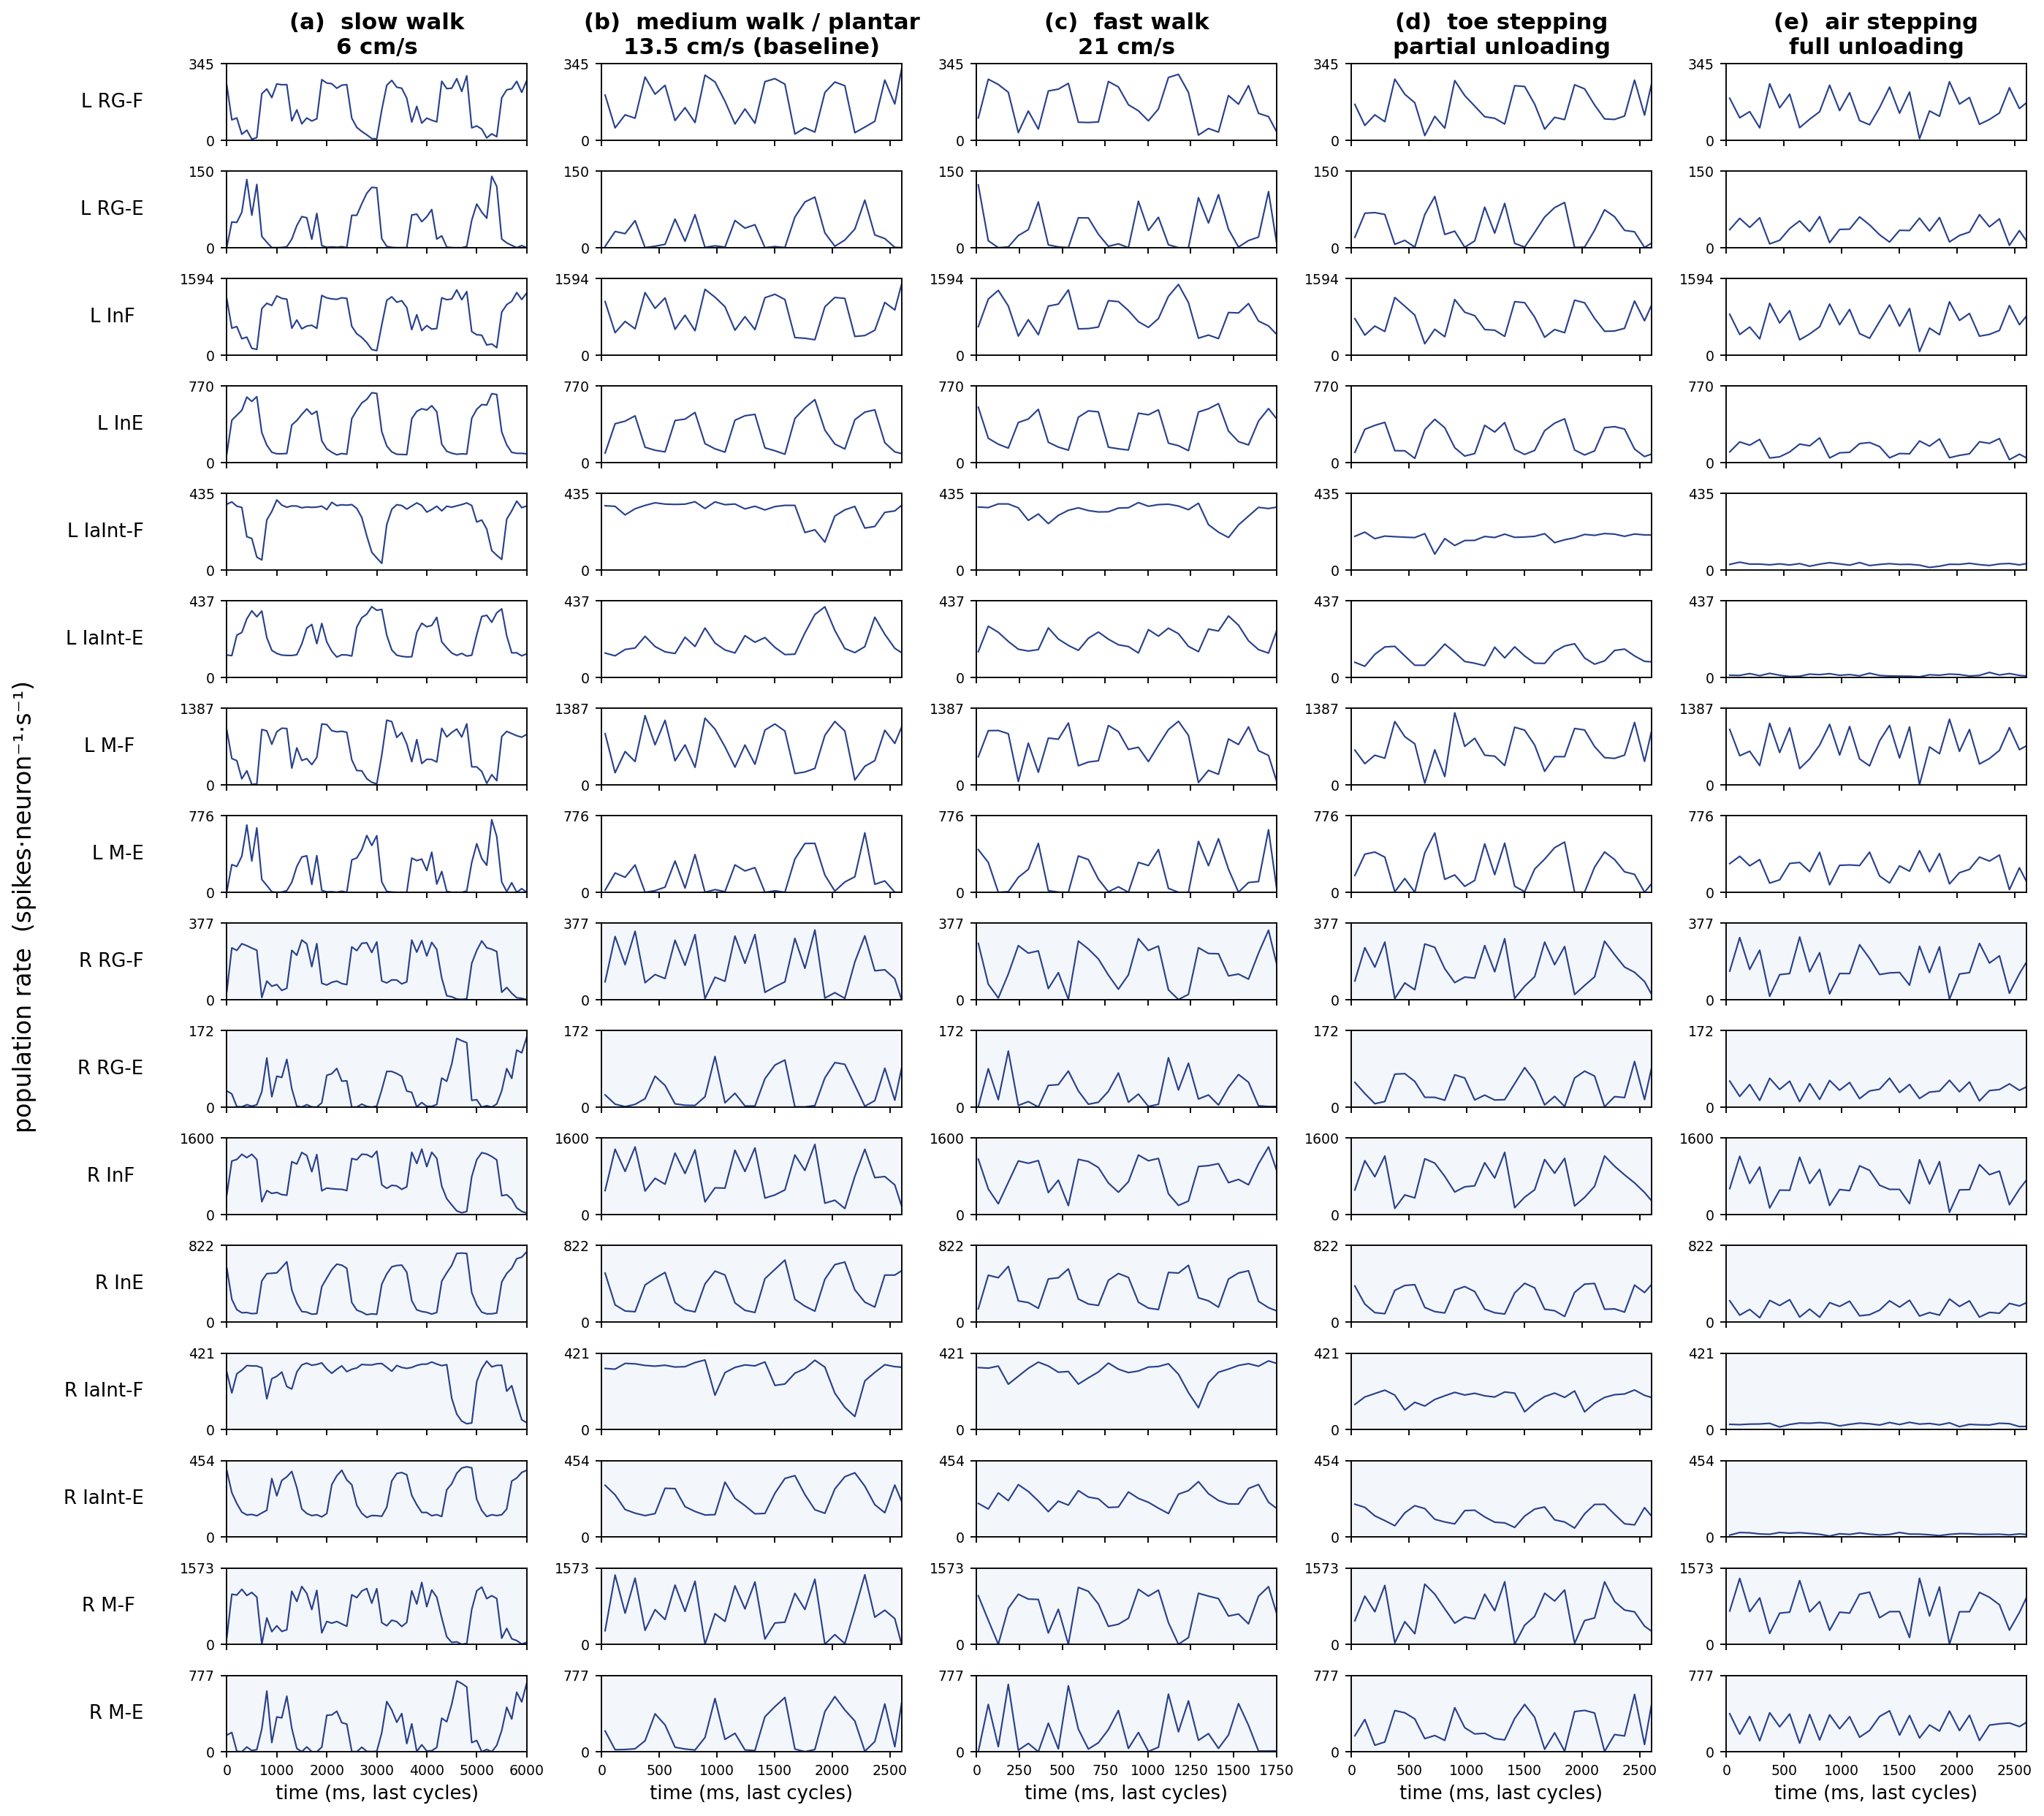
\includegraphics[width=0.95\textwidth]{fig_network_matrix_lam1em6.png}
  \caption{\textbf{Full-circuit population activity, $\lambda=10^{-6}$
    (slowest rate).} Same layout as Figure~\ref{fig:net_l2}.}
  \label{fig:net_l6}
\end{figure}

% =============================================================
\subsection{Comparison across the 5 locomotion modes $\times$ 5 STDP rates}\label{sec:results:comparison}

To compare all twenty-five conditions at a glance, Figures~\ref{fig:mode_lambda_heat}
and~\ref{fig:mode_lambda_trend} and Table~\ref{tab:mode_lambda} reduce each
condition to four numbers (measured over the last $20$\,s of the run): the
alternation of the two muscle forces [corr$(F_E,F_F)$] and of the two rhythm
generators [corr(RG-E,RG-F)] --- both near $-1$ when alternation is clean --- the
peak extensor force, and the final strength of the learned CUT$\to$RG-E synapse.
Three patterns stand out. \textbf{(i) A ``sweet spot'' for the learning rate.}
The final synaptic strength grows steadily with $\lambda$ --- from the
$\approx4$\,pA floor at $10^{-6}$ up to $\approx64$\,pA for $10^{-4}$ and faster
--- but the \emph{quality} of the alternation does not follow suit: it is best at
the intermediate rates and slightly noisier at the very fastest rate, giving a
broad optimum around $\lambda=10^{-3}$--$10^{-4}$. \textbf{(ii) A loading
gradient.} At every learning rate the alternation and the peak force fall as the
limb is unloaded, and under air stepping the muscle-force alternation settles
near $-0.5$ regardless of $\lambda$ --- the withdrawn feedback caps how much
descending drive the network can build. \textbf{(iii) Robustness to walking
speed.} Among the weight-bearing modes the four numbers are almost flat across
speed once learning has converged, showing that the sensory-paced core carries
the gait across the whole rat locomotor range.

\paragraph{Counter-phase \emph{recovers} from toe to air stepping at the
slow learning rates.}
A counterintuitive feature of Figure~\ref{fig:mode_lambda_trend} is that at
the under-converged rates ($\lambda=10^{-5},10^{-6}$) both correlations do not
decrease monotonically with unloading: they are \emph{weakest at toe stepping}
and then \emph{strengthen} again at air stepping (e.g.\ at $\lambda=10^{-6}$,
corr$(F_E,F_F)$ goes $-0.39$ at toe $\to -0.51$ at air, and corr(RG) $-0.74\to
-0.81$), whereas at the fast rates the correlations fall monotonically. This is
the same non-monotonic ``intermediate drive is worst'' effect seen in the
descending-arm learning-rate dependence and in the frozen-weight control: a
\emph{partially}-developed CUT$\to$RG-E weight (toe stepping, where the gated
afferents leave the projection at an intermediate $\approx7$--$18$\,pA) is
strong enough to perturb the paced reciprocal-inhibition core but too weak and
too poorly-timed to cleanly reinforce it, so it desynchronises the rhythm. Under
air stepping the afferents are withdrawn almost entirely (CUT$\to$RG-E gated to
$\approx4$--$8$\,pA), removing that interfering intermediate drive, and the
rhythm reverts to the clean counter-phase \emph{floor} imposed by the paced
heel$\to$toe drive and reciprocal inhibition alone. The paced core therefore
sets a lower bound on counter-phase that the mid-loading, mid-learning regime
can actually fall below.

\paragraph{The RG correlation stays stronger than the force correlation.}
Across the whole matrix corr(RG-E,RG-F) is consistently more negative than
corr$(F_E,F_F)$ --- most visibly under air stepping ($\approx-0.8$ versus
$\approx-0.5$). The rhythm generators keep alternating there because their
antiphase is produced by reciprocal inhibition plus the external pacing, neither
of which requires the plastic drive; what fails under unloading is the
\emph{muscle-force expression} of the extensor. Because the only large plastic
projection is extensor-biased (CUT$\to$RG-E, with no flexor counterpart), gating
the afferents starves the extensor of the activation it needs to develop force,
so the extensor force collapses while the flexor --- intrinsically bursting ---
persists. The counter-phase is thus lost at the muscle level before it is lost
at the rhythm-generator level.

\begin{figure}[t]
  \centering
  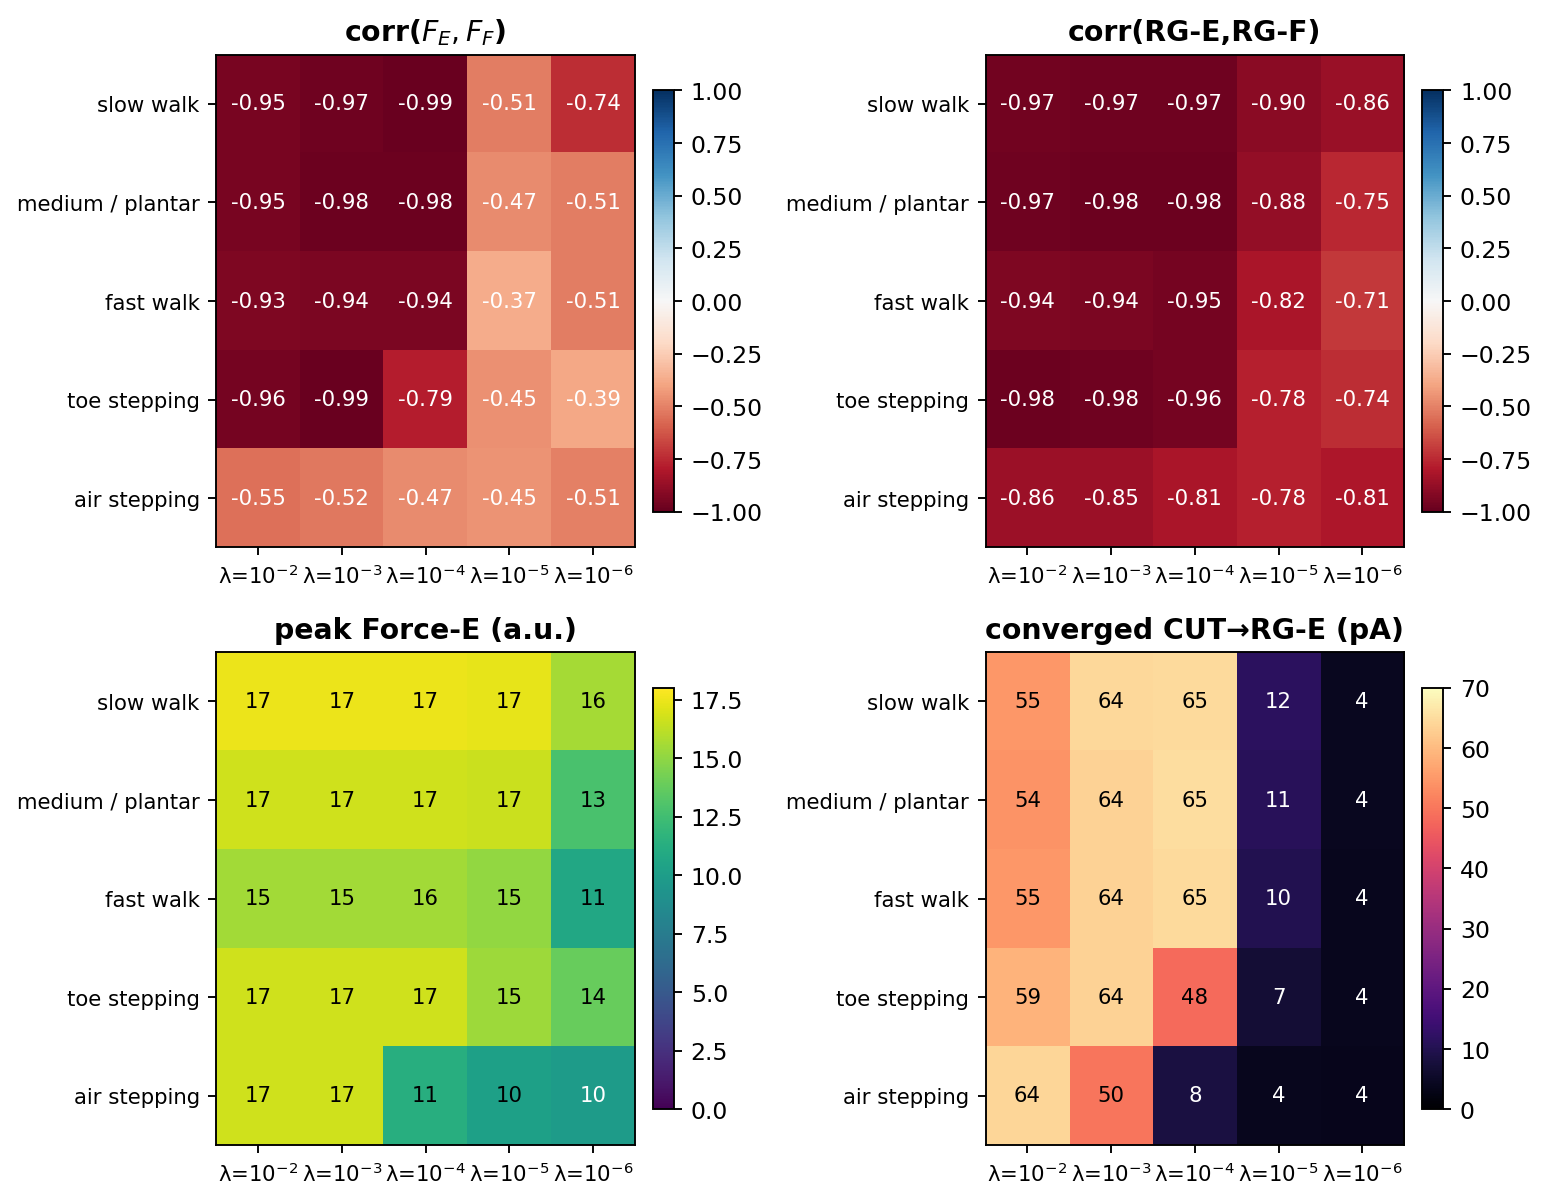
\includegraphics[width=0.95\textwidth]{fig_mode_lambda_heatmaps.png}
  \caption{\textbf{Metric heatmaps across the $5\times5$ rehabilitation-mode
    matrix} (rows: locomotion modes; columns: STDP rate $\lambda$). corr$(F_E,F_F)$
    and corr(RG-E,RG-F) (diverging scale), peak Force-E (a.u.), and converged
    CUT$\to$RG-E weight (pA). Last-20\,s window, canonical sensory model.}
  \label{fig:mode_lambda_heat}
\end{figure}

\begin{figure}[t]
  \centering
  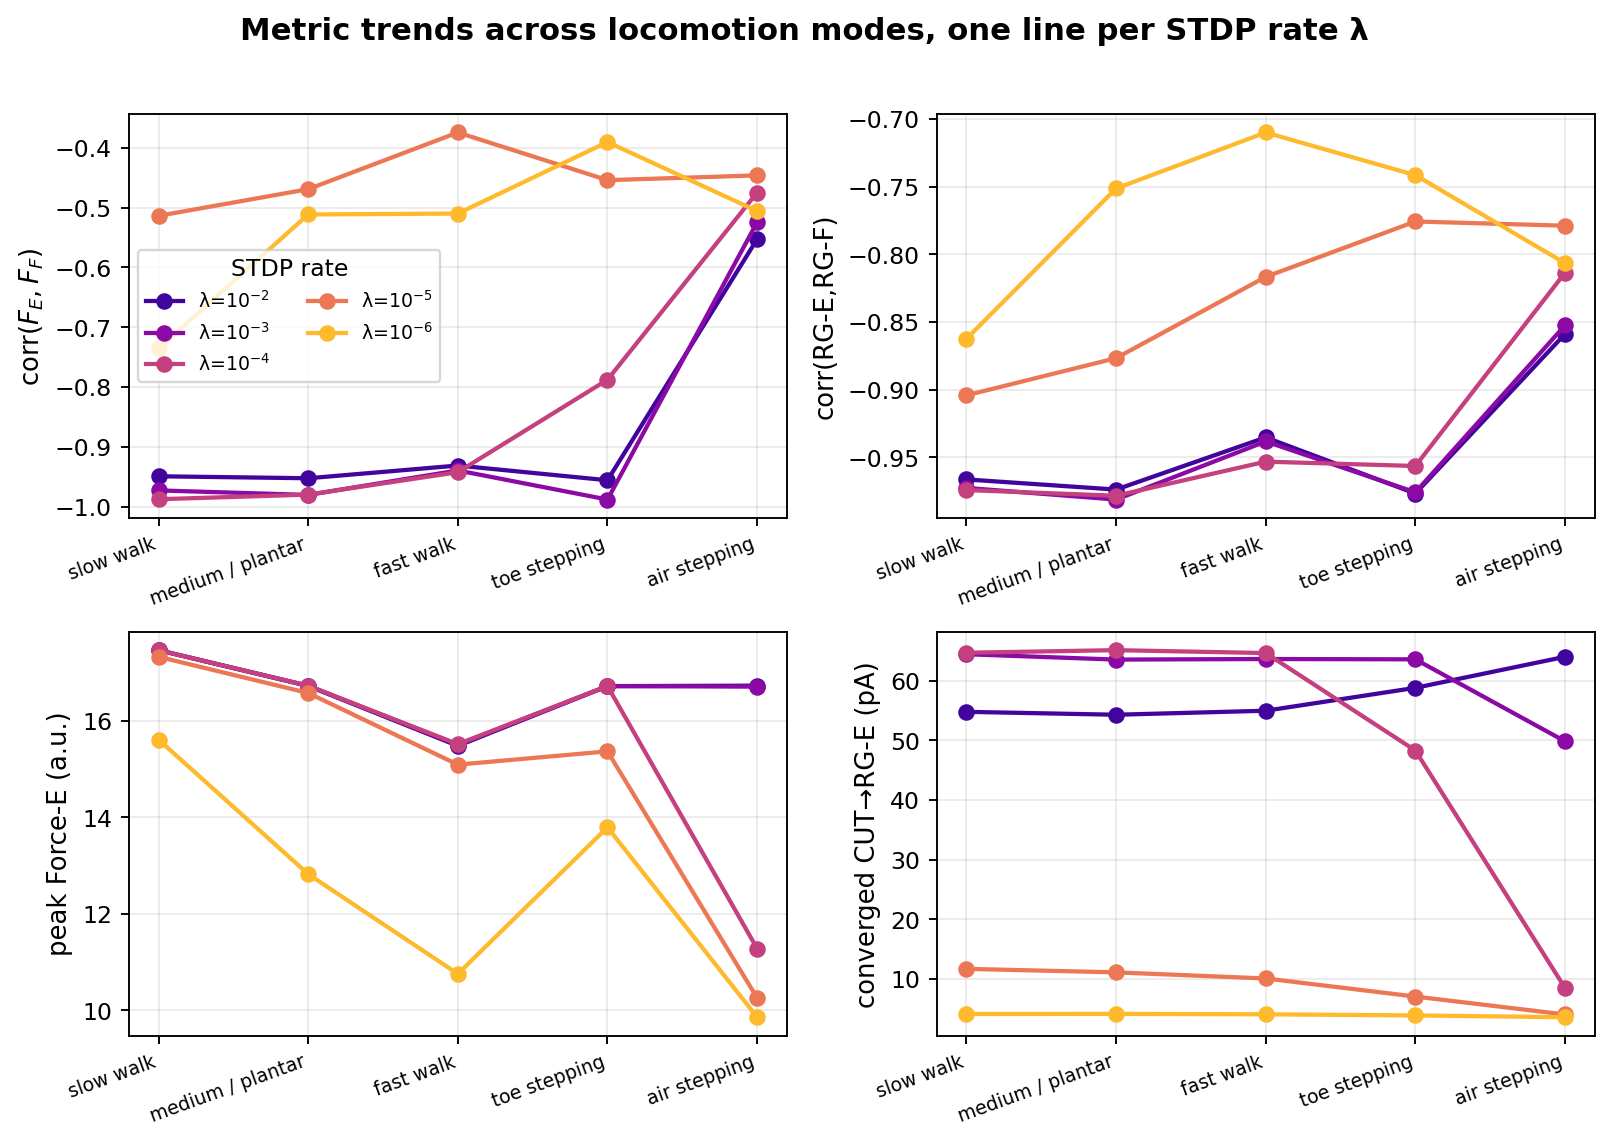
\includegraphics[width=0.9\textwidth]{fig_mode_lambda_trends.png}
  \caption{\textbf{Metric trends across the locomotion modes, one line per STDP
    rate $\lambda$.} Same four metrics as Figure~\ref{fig:mode_lambda_heat},
    plotted against the locomotion mode (slow walk $\to$ air stepping) to expose
    the loading gradient and the learning-rate ordering.}
  \label{fig:mode_lambda_trend}
\end{figure}

\input{mode_lambda_table}

% =============================================================
\subsection{Epidural stimulation rescues stepping under unloading}\label{sec:results:epidural}

Finally, the model speaks to a striking clinical observation: people and animals
with severe spinal cord injury often cannot step on their own, yet regain
stepping when the lumbar spinal cord is electrically stimulated (\emph{epidural
stimulation}). We reproduce the two situations by choosing how the paw-contact
drive behaves under unloading (Figure~\ref{fig:epidural}). In the \emph{natural}
(unassisted) case both the cutaneous and the proprioceptive feedback fade
together as the limb is unloaded, and the rhythm collapses (muscle-force
correlation $-0.41$ at air stepping, with the cycle period also becoming
irregular). When the rhythmic cutaneous drive is instead held on regardless of
loading --- the model's stand-in for epidural stimulation, which supplies a
rhythmic input that does not depend on limb
contact~\cite{courtine2009,harkema2011} --- the alternation is preserved across
the whole loading range (correlation $-0.94$ at baseline to $-0.97$ at air
stepping). This double dissociation
captures the mechanism behind the clinical finding that motor-complete subjects
cannot step unassisted but recover treadmill stepping under epidural
stimulation~\cite{courtine2009,harkema2011}.

\begin{figure}[t]
  \centering
  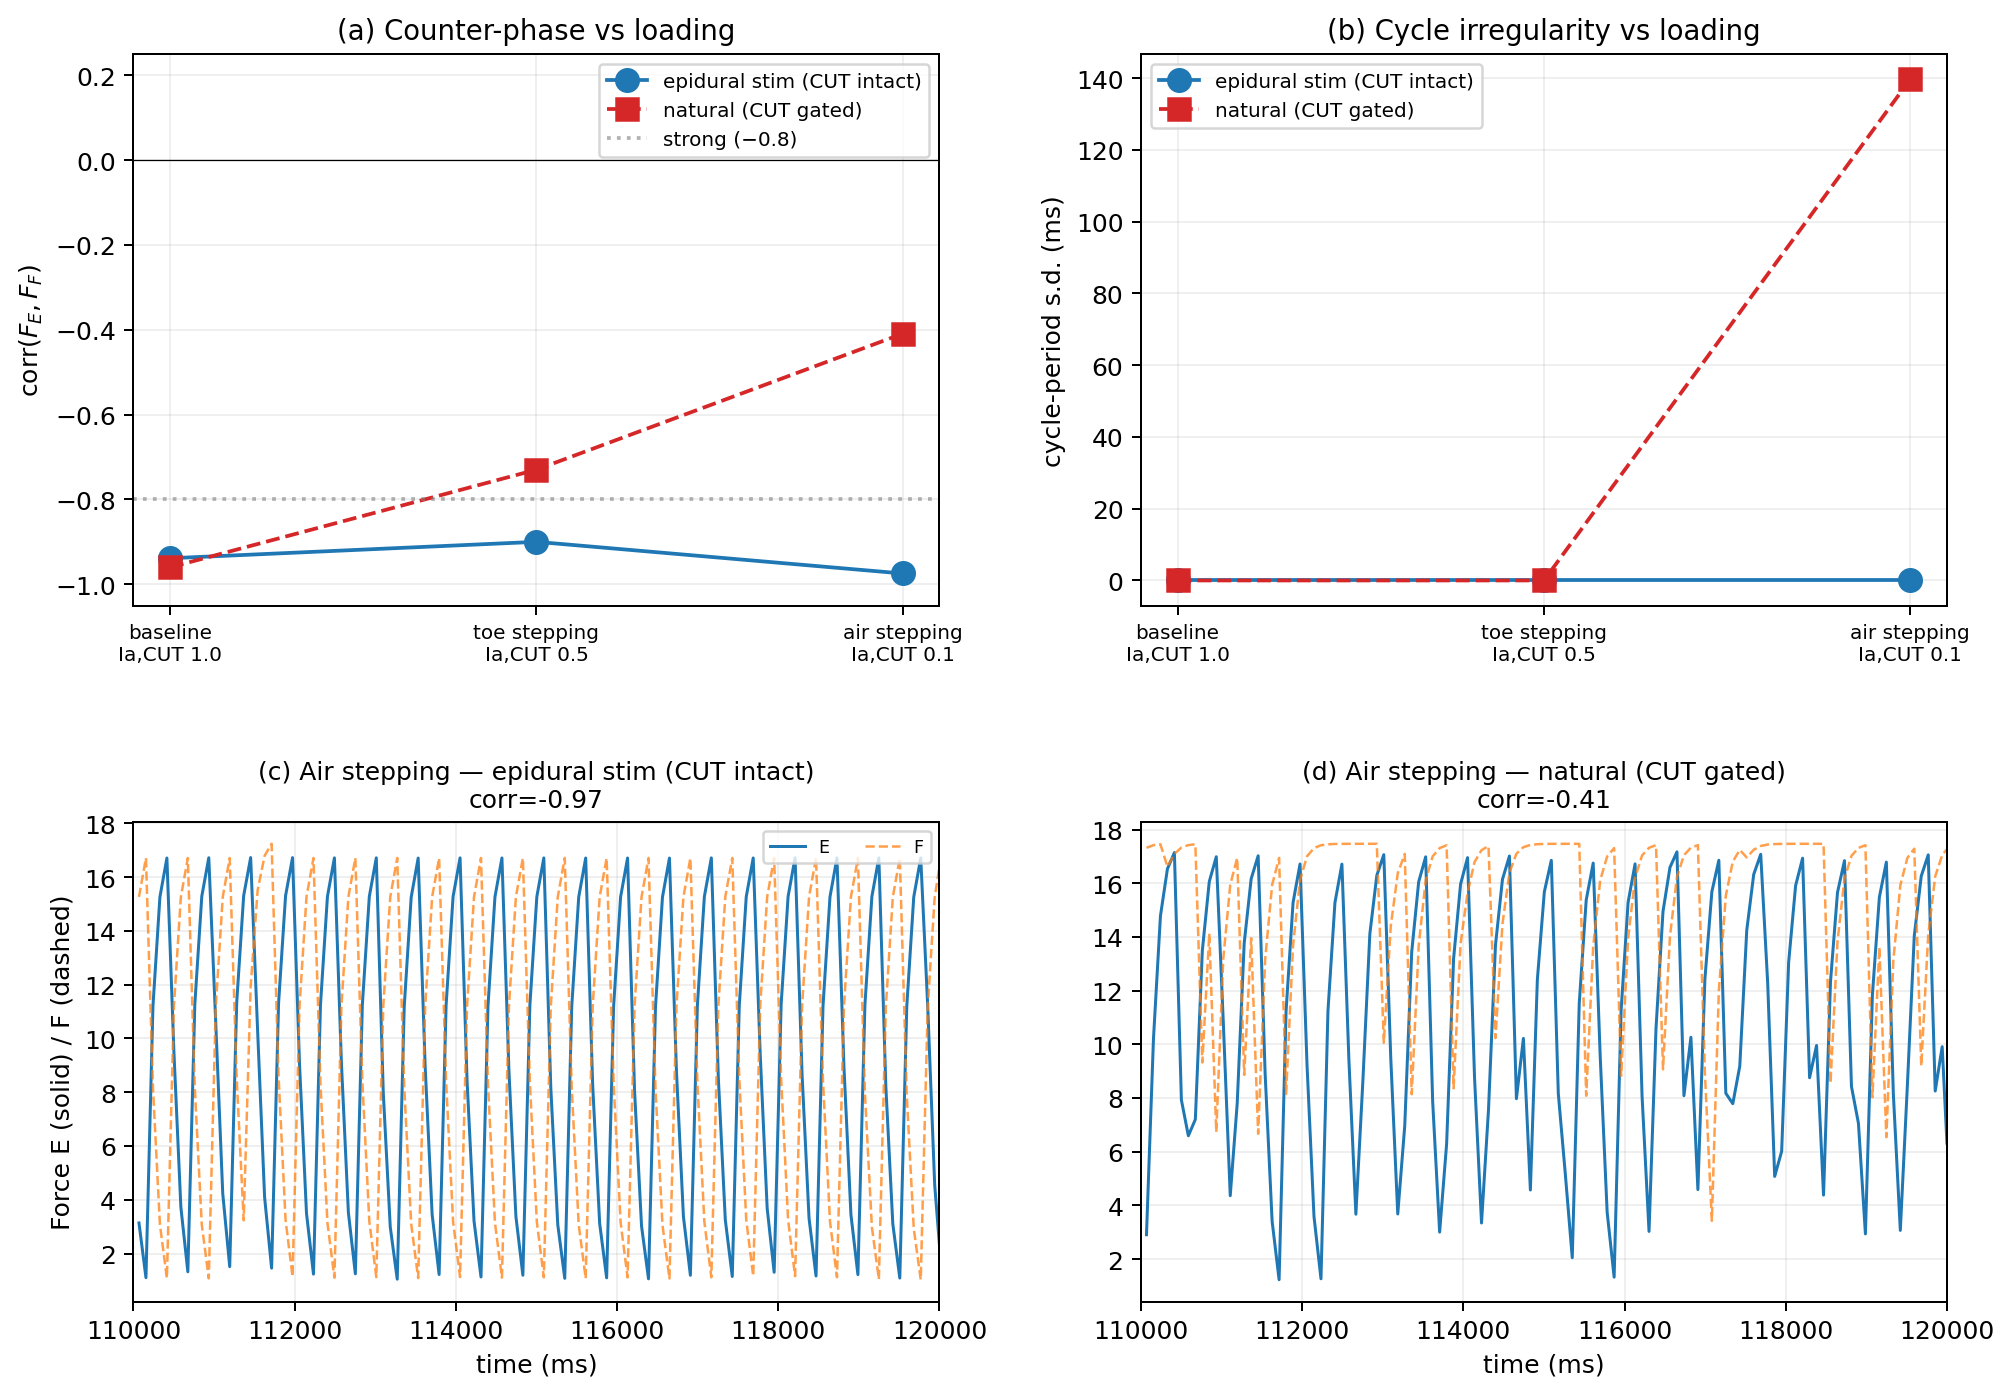
\includegraphics[width=0.8\textwidth]{fig9_epidural_contrast.png}
  \caption{\textbf{Epidural-stimulation rescue --- paced cutaneous drive
    preserves stepping under unloading.} Loading swept from baseline to air
    stepping. \textbf{(a)} counter-phase corr$(F_E,F_F)$ versus loading:
    epidural-stim (CUT held intact) stays strong, the natural (CUT gated) arm
    collapses. \textbf{(b)} cycle-period jitter versus loading.
    \textbf{(c, d)} representative air-stepping force traces for the stim and
    natural arms.}
  \label{fig:epidural}
\end{figure}

% =============================================================
\subsection{Closed-loop force-triggered stepping and tag-and-capture
  consolidation}\label{sec:results:consolidate}

\emph{Debug-scale, preliminary: a full production-scale (N=100, brainstem
input at 60\,Hz) confirmatory sweep has been prepared for submission to an
HPC cluster, and every figure in this subsection will be replaced with the
production-scale equivalent once it completes; the qualitative pattern
reported here is not expected to change, but the numbers are debug-scale
(reduced population size, 20\,Hz brainstem input) and should be read
accordingly.}

The results above drive stance/swing timing with an explicit clock. We also
built a closed-loop alternative in which cutaneous (paw-contact) firing is
gated directly on each leg's own extensor force: contact turns on when force
rises through 80\% of that stride's peak and turns off when it falls back
through 35\%, so the rhythm is generated by the mechanics of stepping itself
rather than imposed on it. Because the extensor rhythm generator has no
intrinsic burst-terminating current, a fixed-duration failsafe (matched to
the model's own $\approx450$\,ms stance target) forces the phase transition
if the force-threshold crossing is late; we track the fraction of strides
that hit this failsafe (`frac\_at\_cap`) as a direct check on whether a given
configuration is a genuine closed loop or a disguised clock wearing a
force-shaped costume.

\paragraph{Five locomotion modes, two learning architectures.} We confirmed
two additional timing points bracketing the original one --- a
$\approx31\%$ slower and a $\approx13$--$18\%$ faster variant --- found by
scaling the stance-duration and muscle-fatigue time constants together
rather than moving any one parameter alone. The faster point needed one
further ingredient: a small, \emph{persistent} left/right asymmetry in the
muscle-fatigue time constant (the leading leg fatigues slightly faster
than the other, for the whole run, not just at the initial symmetry-breaking
step). Without it, several otherwise-genuine fast configurations settled
into a perfectly regular cycle whose left/right phase relationship
(alternating vs.\ moving together) was decided by run-to-run noise rather
than by any timing parameter; the persistent asymmetry --- itself
bio-plausible, since real limbs are not identical --- reliably resolves
this bistability. We crossed both walking-speed points, plus the original
medium speed, with the two ablation loading levels used throughout this
paper (toe and air stepping, partial and full unloading) and the two
learning architectures: a \emph{descending} arm in which the
brainstem-to-rhythm-generator synapse remains plastic (as in the results
above), and a \emph{sensory} arm in which that synapse is frozen at a weak
fixed value and only the cutaneous and proprioceptive afferent synapses
learn --- the model's stand-in for a rehabilitation scenario in which
descending drive is compromised but peripheral feedback pathways are intact.

Figure~\ref{fig:ct_all_modes_force} shows all three walking speeds and toe
stepping produce a genuine, closed-loop counter-phase rhythm in both
architectures (corr$(F_E,F_F)=-0.53$ to $-0.90$ at the three speeds,
$-0.23$ to $-0.84$ at toe stepping, weakening but not collapsing under
partial unloading as expected). Air stepping is the exception, and
deliberately so: force stays too small for the closed-loop threshold
mechanism to find any genuine crossings, so cutaneous drive never
develops (Figure~\ref{fig:ct_all_modes_weights}, right column) and the
rhythm degrades toward the tick resolution of the simulation --- the
same natural-air-stepping collapse already reported in
Section~\ref{sec:results:epidural} under the fixed clock, now reproduced
under closed-loop timing instead of imposed by construction. We do not
attempt to force a clean rhythm out of natural air stepping here; the
model's own epidural-stimulation rescue (Section~\ref{sec:results:epidural})
is the appropriate comparison condition for that, not a retuned threshold.
Figure~\ref{fig:ct_all_modes_weights} shows the CUT$\to$RG-E weight
converging to the same $\approx60$--$67$\,pA plateau at every walking speed
and at toe stepping, in both architectures --- the same
initialization-independent set-point reported in
Section~\ref{sec:results:weights}, now shown to hold under closed-loop
timing as well as the fixed clock, across a substantially wider range of
speeds and loading than the single operating point first confirmed for
this mechanism.

\begin{figure}[t]
  \centering
  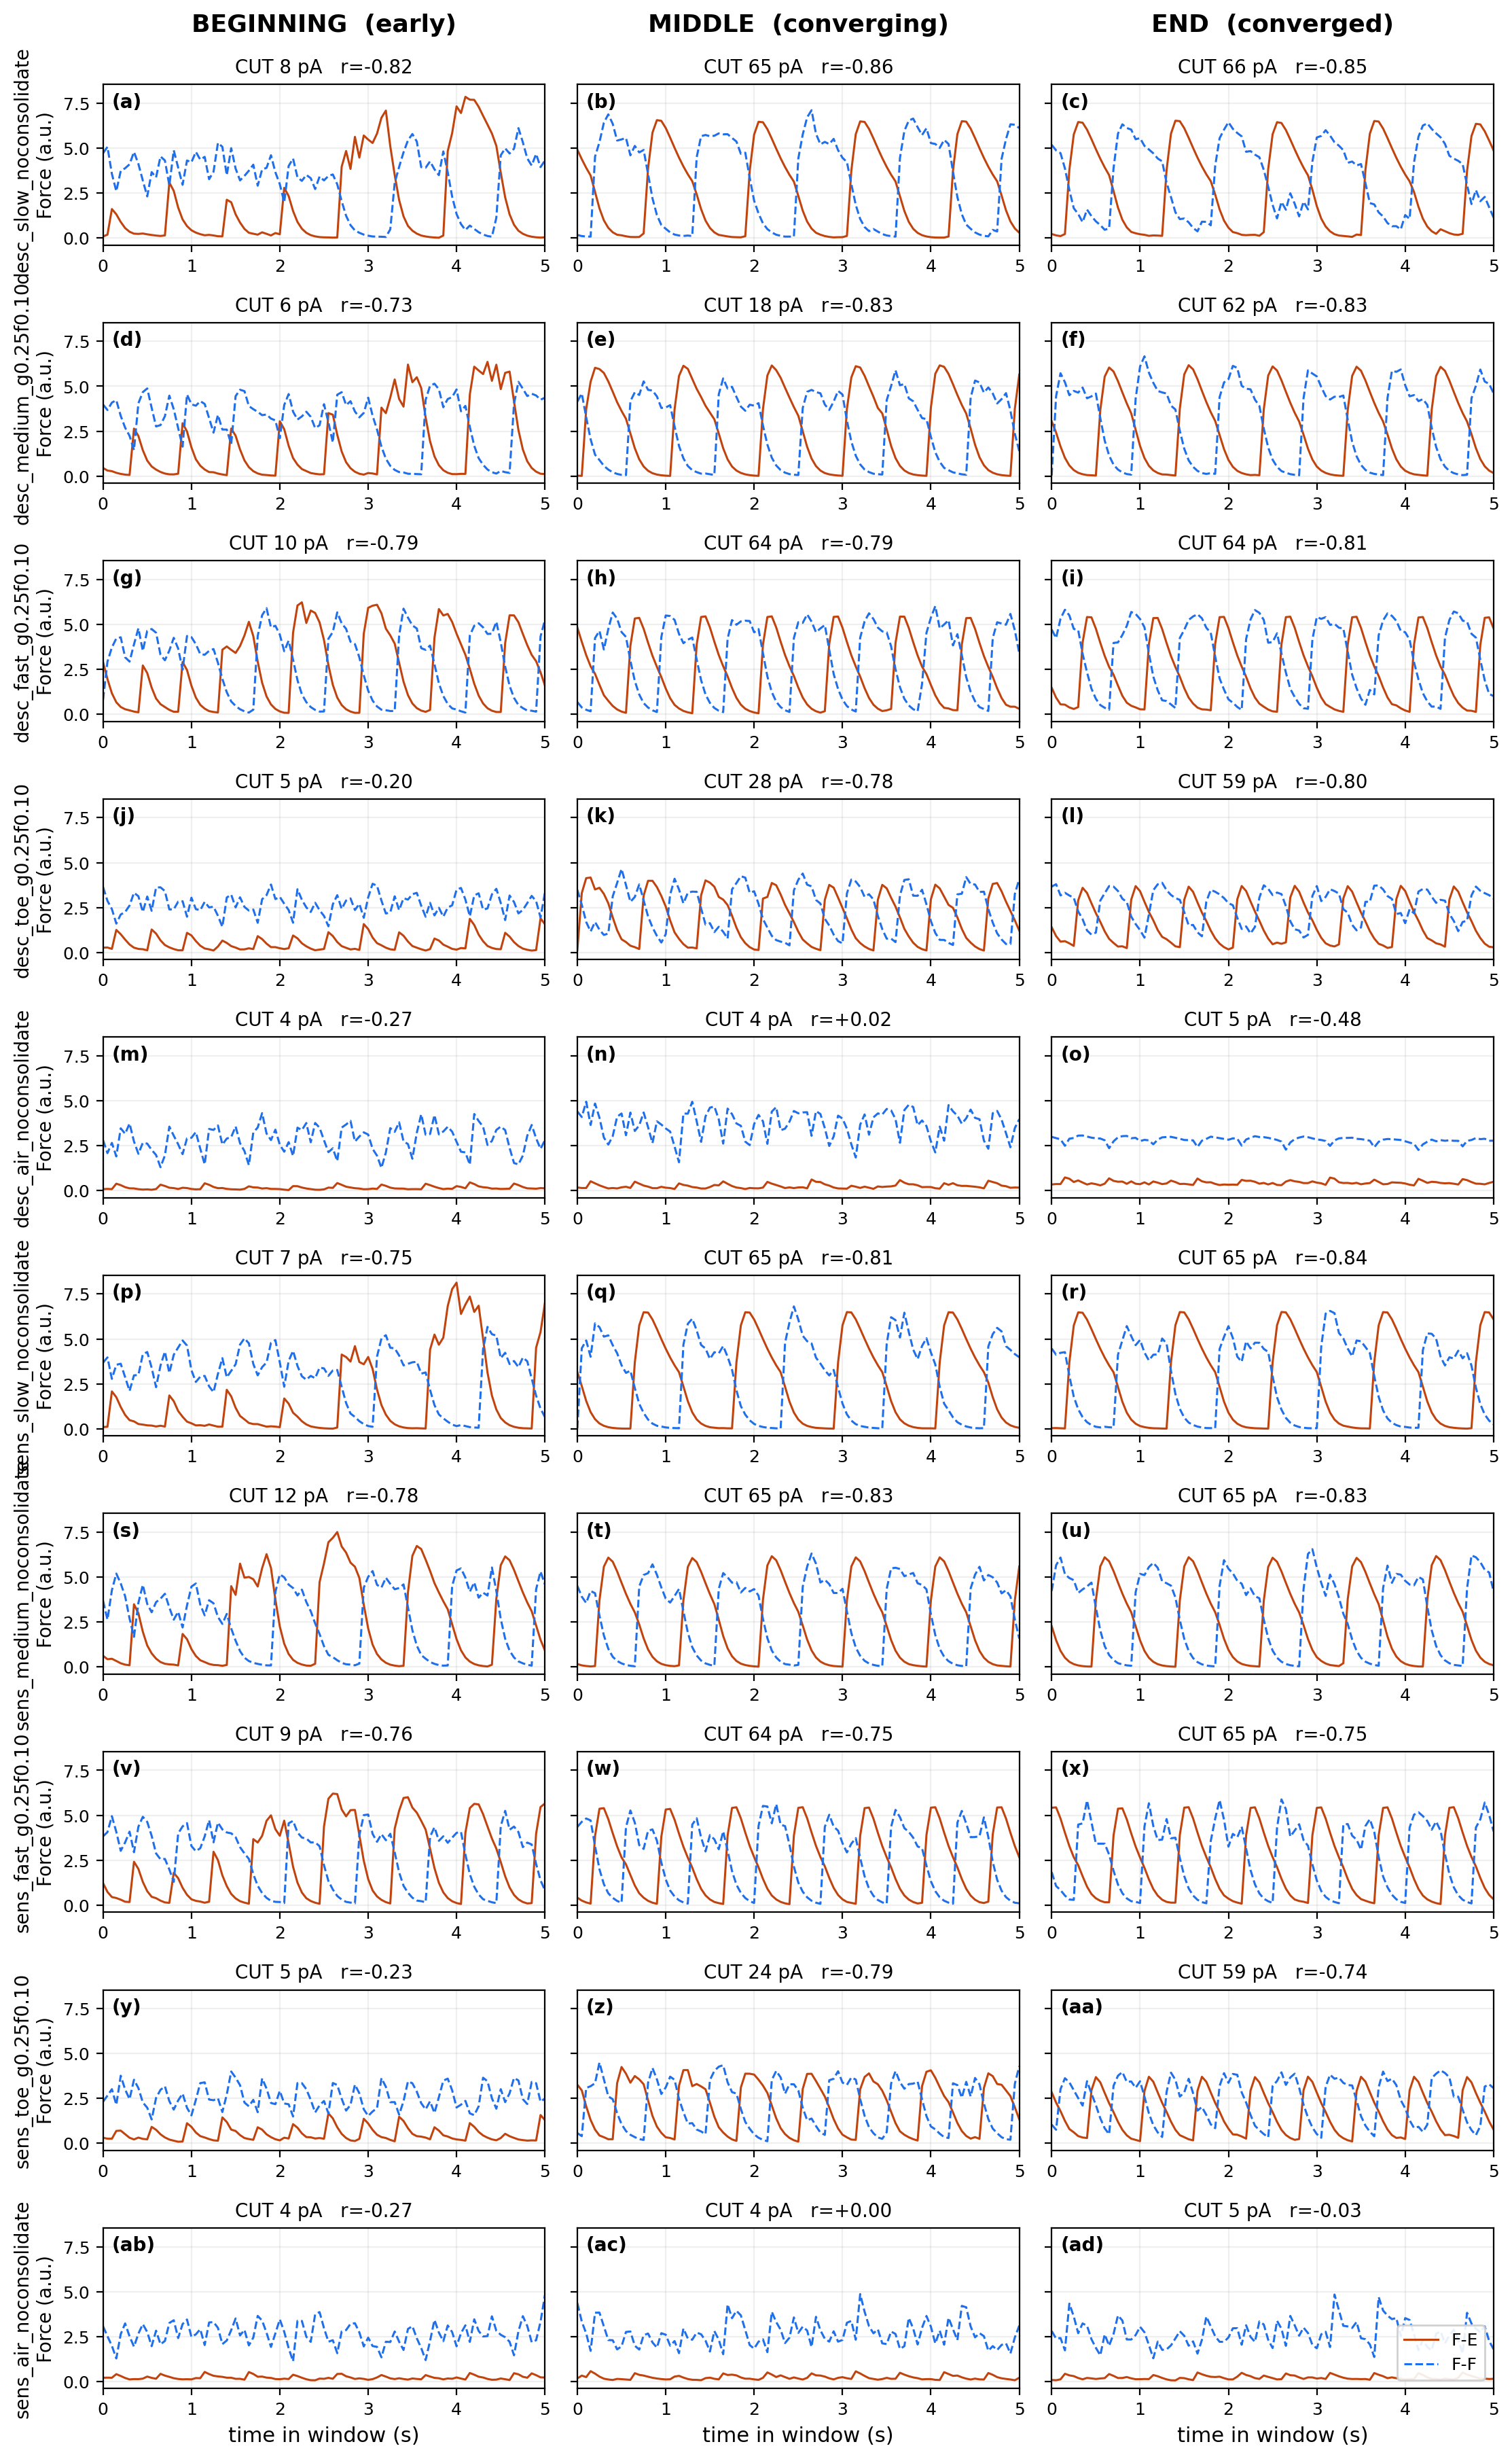
\includegraphics[width=0.92\textwidth]{fig_forcetrigger_all_modes_force_stages.png}
  \caption{\textbf{Closed-loop (force-triggered) stepping across all five
    locomotion modes and both learning architectures.} Rows (top to
    bottom): descending arm at slow/medium/fast/toe/air, then sensory arm
    at slow/medium/fast/toe/air; columns: beginning / middle / end of the
    $60$\,s run, as in Figure~\ref{fig:force_l2}. Air stepping (rows 5, 10)
    shows the expected natural collapse, not a fitting failure. Panels
    (a)--(ad).}
  \label{fig:ct_all_modes_force}
\end{figure}

\begin{figure}[t]
  \centering
  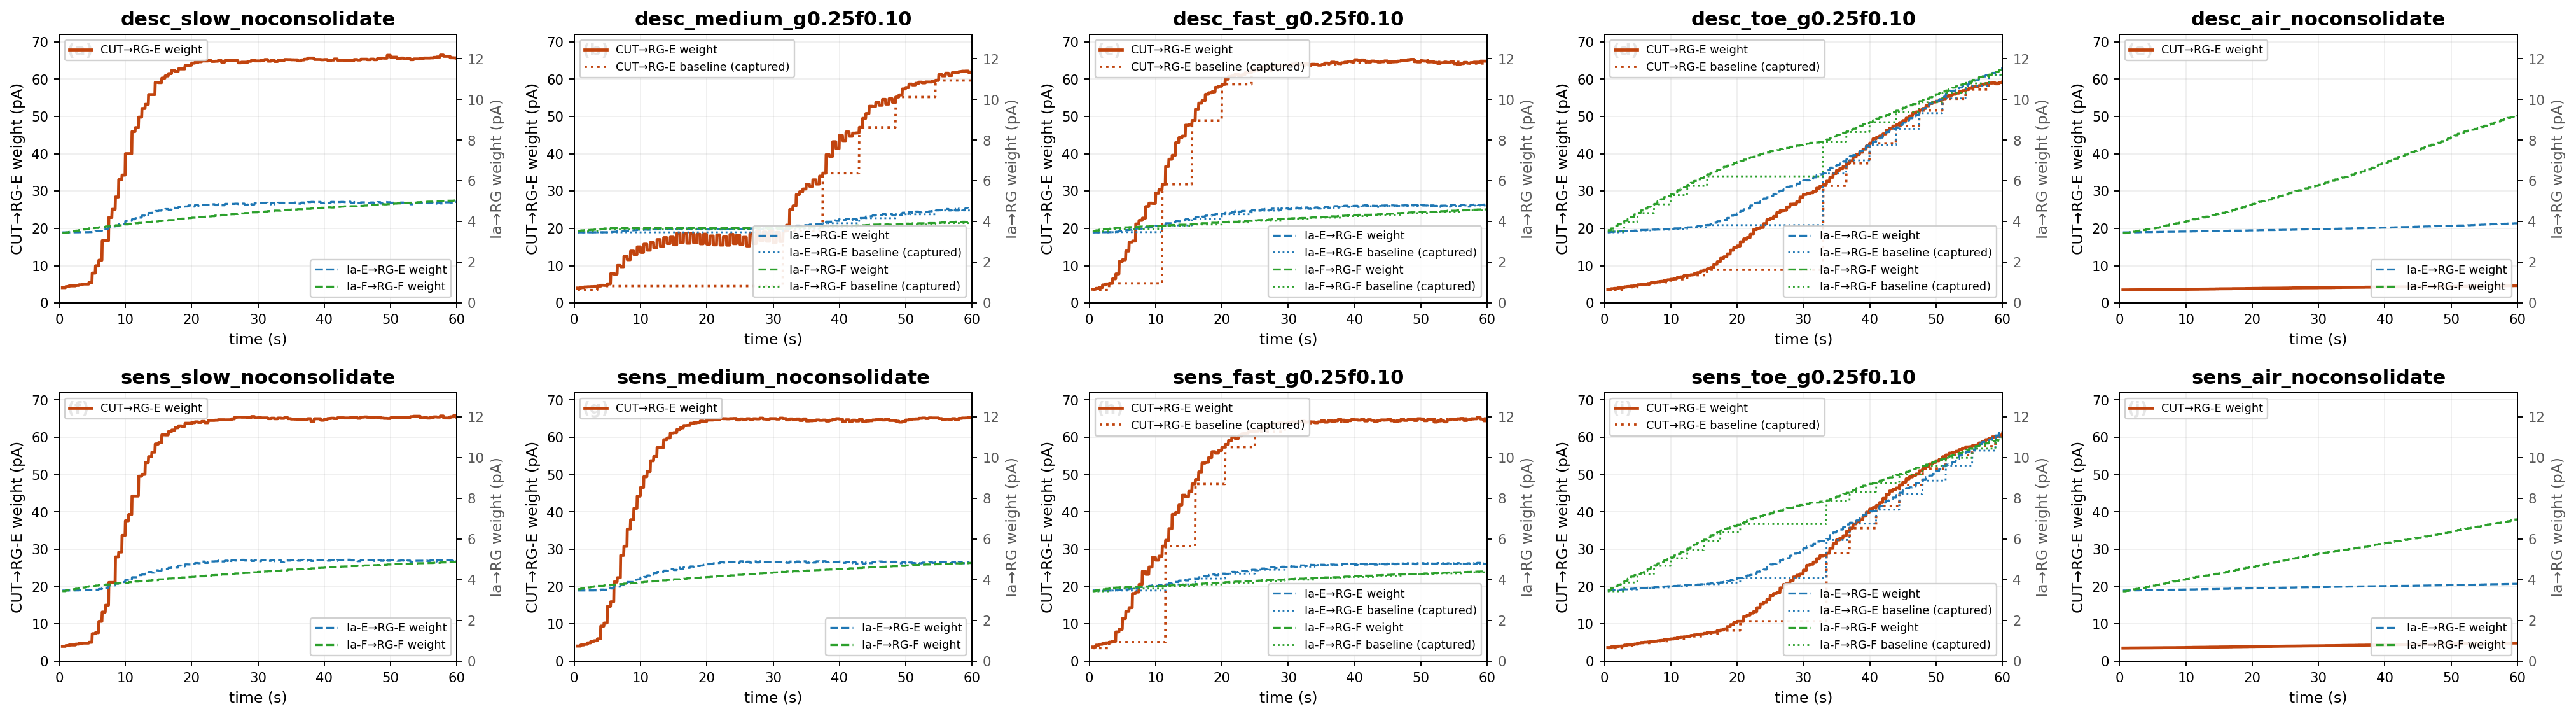
\includegraphics[width=0.98\textwidth]{fig_forcetrigger_all_modes_weights_grid.png}
  \caption{\textbf{The learned set-point is the same across speeds and
    loading levels, except where force never develops.} CUT$\to$RG-E
    weight (solid, left axis; dotted = captured baseline where
    consolidation, below, is active --- medium, fast and toe rows, all at
    the same confirmed gain; slow and air run without consolidation, see
    text) and Ia-E/F$\to$RG weights (dashed, right axis) versus time, one
    panel per condition from Figure~\ref{fig:ct_all_modes_force}. Toe
    stepping's Ia$\to$RG weights climb further than at full loading (a
    loading-dependent relaxation of the Ia$\to$RG weight ceiling lets
    proprioceptive feedback take over more excitatory drive as cutaneous
    input is progressively removed); air stepping's CUT$\to$RG-E rises only
    slowly and by a small amount over the run, well short of the
    $\approx60$--$67$\,pA plateau reached elsewhere.}
  \label{fig:ct_all_modes_weights}
\end{figure}

\paragraph{Tag-and-capture consolidation.} Vanilla STDP retains every
potentiation permanently, up to its ceiling, with no way to distinguish a
genuine, force-threshold-driven stride from one only completed because the
failsafe forced it. We therefore added an optional consolidation layer,
directly analogous to synaptic tagging-and-capture in hippocampal memory
models \todo{cite Sandkuhler spinal E-LTP/L-LTP; Grau contingency-gated
spinal learning; Wolpaw two-phase H-reflex conditioning}: each plastic
connection keeps its native STDP weight (the fast, local ``tag'') alongside
a separate, slower-changing \emph{baseline}. A shared per-leg pool
accumulates from genuine stride endings and is drawn down by failsafe-forced
ones; only once it crosses a threshold does the baseline snap to the current
weight (a \emph{capture} event), and between captures the live weight
continuously relaxes back toward the baseline. The weight ceiling itself is
untouched --- this mechanism governs what is \emph{retained} within the
existing ceiling, not the ceiling.

\todo{Revision note, to resolve before submission: the medium-speed
timing point used to illustrate this mechanism was found to have 4 of its
5 timing constants landing exactly on the simulation's discretization
step, which let its stance/swing timing collapse onto seed- and
thread-sensitive discrete states independently of consolidation. A small
($\approx1\%$) de-alignment of two constants fixed this for the base
(non-consolidated) mechanism. Separately, the bookkeeping for the
brainstem-to-rhythm-generator pathway was tracked but never written back
to the simulator, so that pathway ran unconsolidated (ordinary STDP)
regardless of this mechanism being enabled, for every result reported
below at the time this note was written. Both issues are now fixed, and
the gain search below was re-run afterward; the numbers and figures in
this subsection reflect the corrected code, but only at reduced network
size (debug scale) --- a full-scale confirmatory run is in progress.
Remove this note once that confirmation lands and the numbers below are
verified to match at full scale.}

One gain setting (how strongly a genuine vs.\ a forced stride moves the
pool) was identified by grid search and confirmed across two random
seeds, and applies uniformly across all three walking speeds and both
learning architectures: $0.25$ for a genuine stride, $0.10$ for a
failsafe-forced one. This supersedes an earlier finding of two
architecture-specific settings, an artifact of the two issues noted above
rather than a genuine property of the two learning architectures.
Figure~\ref{fig:consolidate_desc} shows the descending arm:
without consolidation the weight is retained unconditionally regardless of
how it was earned; at a forced-favoring gain (the reverse ratio, forced
outweighing genuine 3:1) the pool never crosses threshold and the
mechanism is an inert no-op --- notably, the brainstem-to-rhythm-generator
pathway is visibly suppressed here too (converging far below its
unconsolidated plateau) even though it never captures, since the
continuous tag-decay this mechanism applies runs whether or not a capture
ever happens; at the confirmed gain the baseline visibly steps upward each
time enough genuine strides accumulate
(Figure~\ref{fig:consolidate_desc_weights}), and all three plastic
pathways --- including the brainstem projection --- converge to a stable
captured value.

\begin{figure}[t]
  \centering
  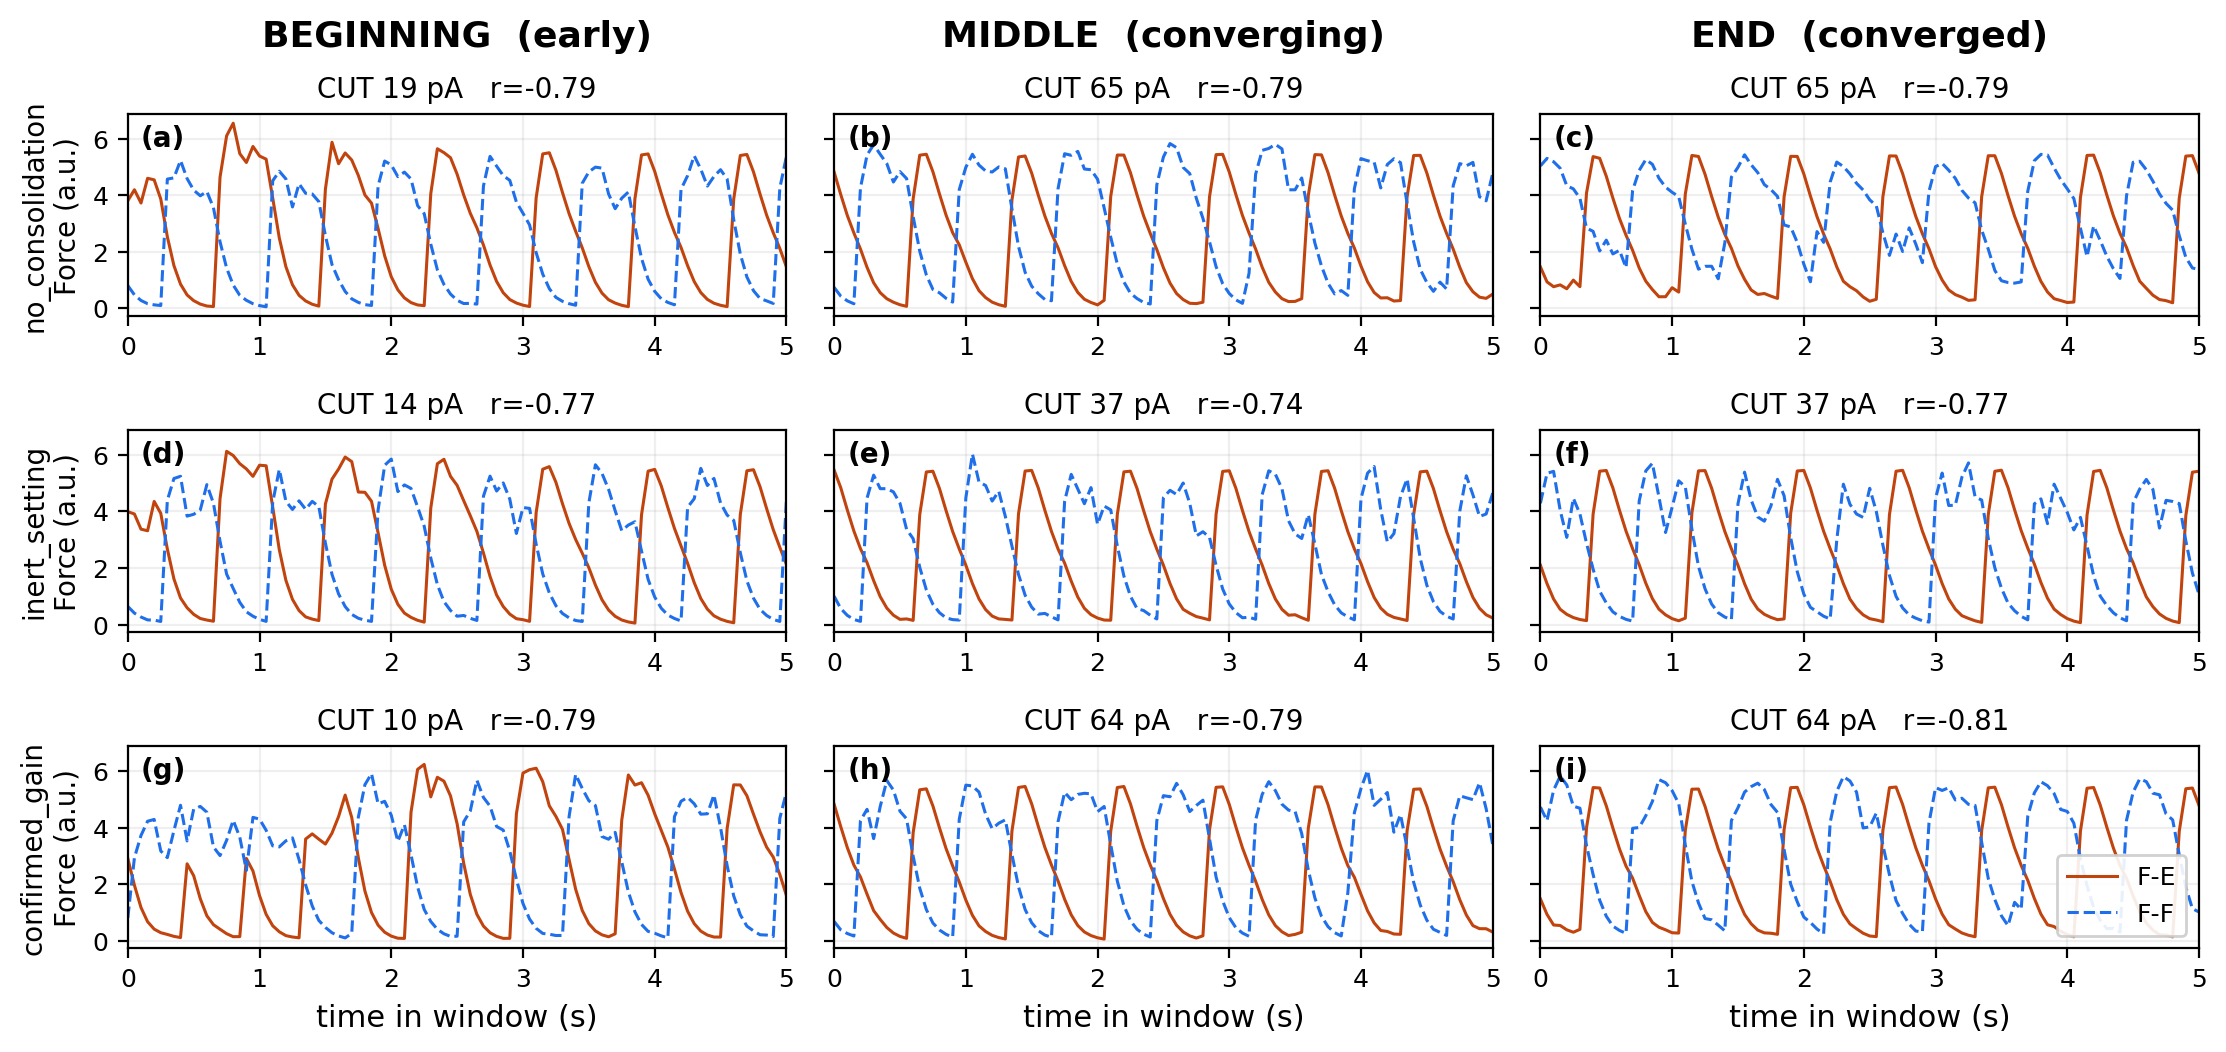
\includegraphics[width=0.92\textwidth]{fig_consolidate_descending_force_stages.png}
  \caption{\textbf{Tag-and-capture consolidation, descending arm.} Rows:
    no consolidation; an inert (never-captures) gain setting ($0.15$
    genuine / $0.30$ forced); the confirmed working gain ($0.25$ genuine /
    $0.10$ forced). Columns as in Figure~\ref{fig:ct_all_modes_force}.
    Panels (a)--(i).}
  \label{fig:consolidate_desc}
\end{figure}

\begin{figure}[t]
  \centering
  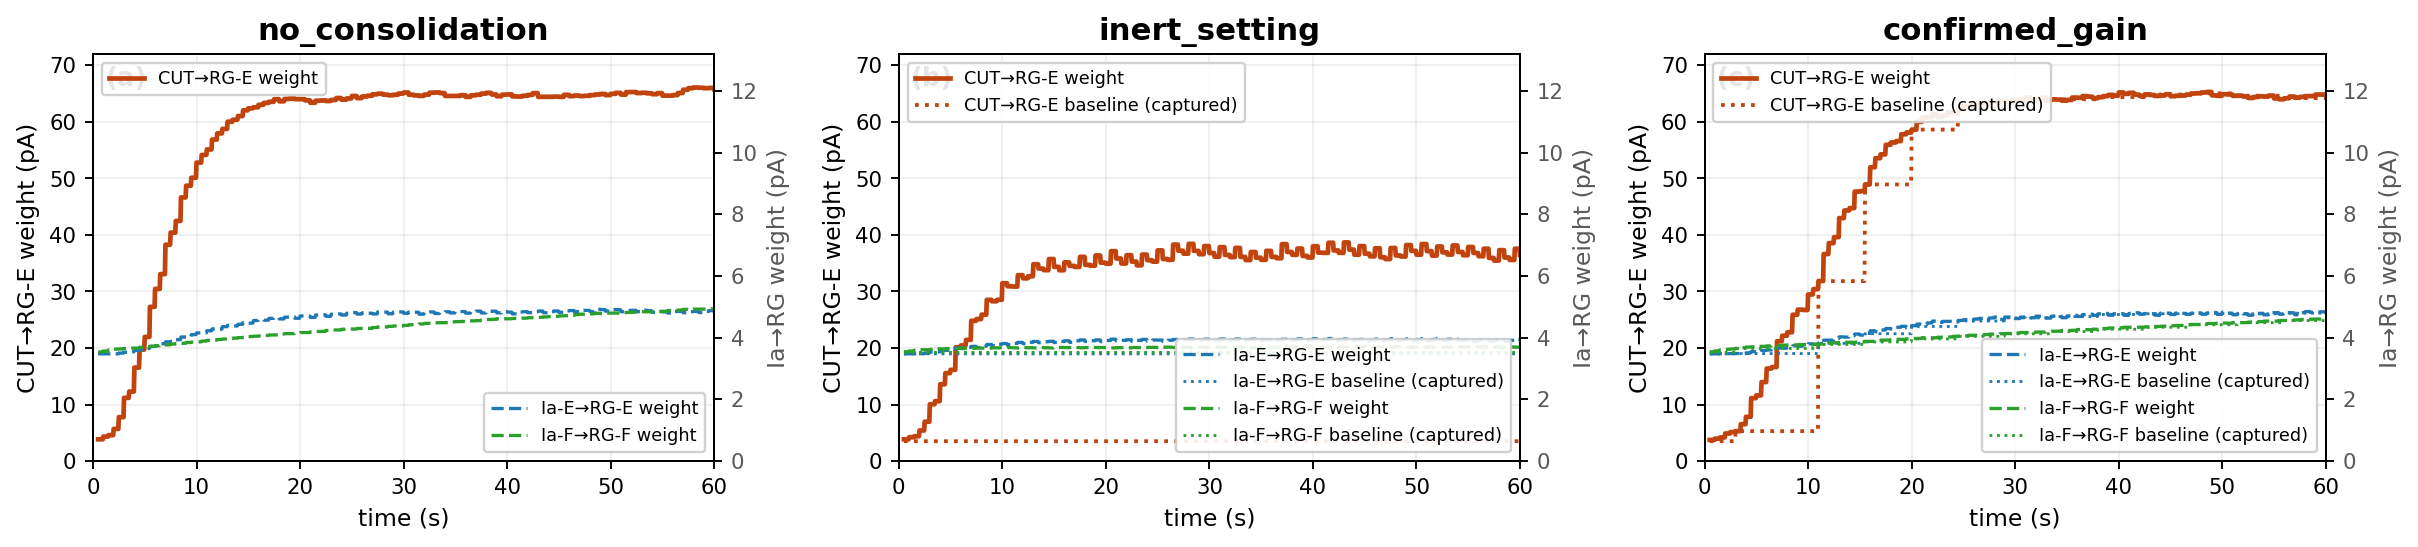
\includegraphics[width=0.95\textwidth]{fig_consolidate_descending_weights_grid.png}
  \caption{\textbf{The capture staircase, now spanning all three plastic
    pathways.} Solid/dashed = live STDP weight; dotted = captured baseline
    (only present once consolidation is on). Left: no consolidation (no
    baseline to show). Middle: inert setting --- baseline frozen at
    initialization despite the live weight moving, on every pathway
    including the brainstem projection. Right: confirmed working gain ---
    baseline steps upward at each capture event and tracks the live
    weight's converged value by the end of the run, again on all three
    pathways.}
  \label{fig:consolidate_desc_weights}
\end{figure}

\paragraph{The same gain also works for the sensory arm.} Earlier testing,
before the two fixes noted above, had found the descending arm's gain
setting synchronized the legs when applied to the sensory arm instead, and
concluded the two architectures needed different settings. That
conclusion does not hold once the two fixes are applied: the confirmed
gain (Figure~\ref{fig:consolidate_sens}) captures cleanly in the sensory
arm too, converging both legs' cutaneous synapse to a captured baseline
(Figure~\ref{fig:consolidate_sens_weights}) without reproducing the
earlier synchronization failure. \todo{Revision note: a bout-timeline figure previously illustrated a
settling-in transient at run start (an extended run of failsafe-forced
strides early on that resolves to genuine timing before the run ends,
motivating the steady-state-only convention used throughout this
subsection). That figure and claim are removed here pending
re-verification: the operating point used to demonstrate it has changed
along with everything else in this subsection, and a first check on the
new fast-timing point found no such transient (steady from the start), so
the original claim should not be carried forward uncritically. Re-add once
a current, verified version exists.}

\begin{figure}[t]
  \centering
  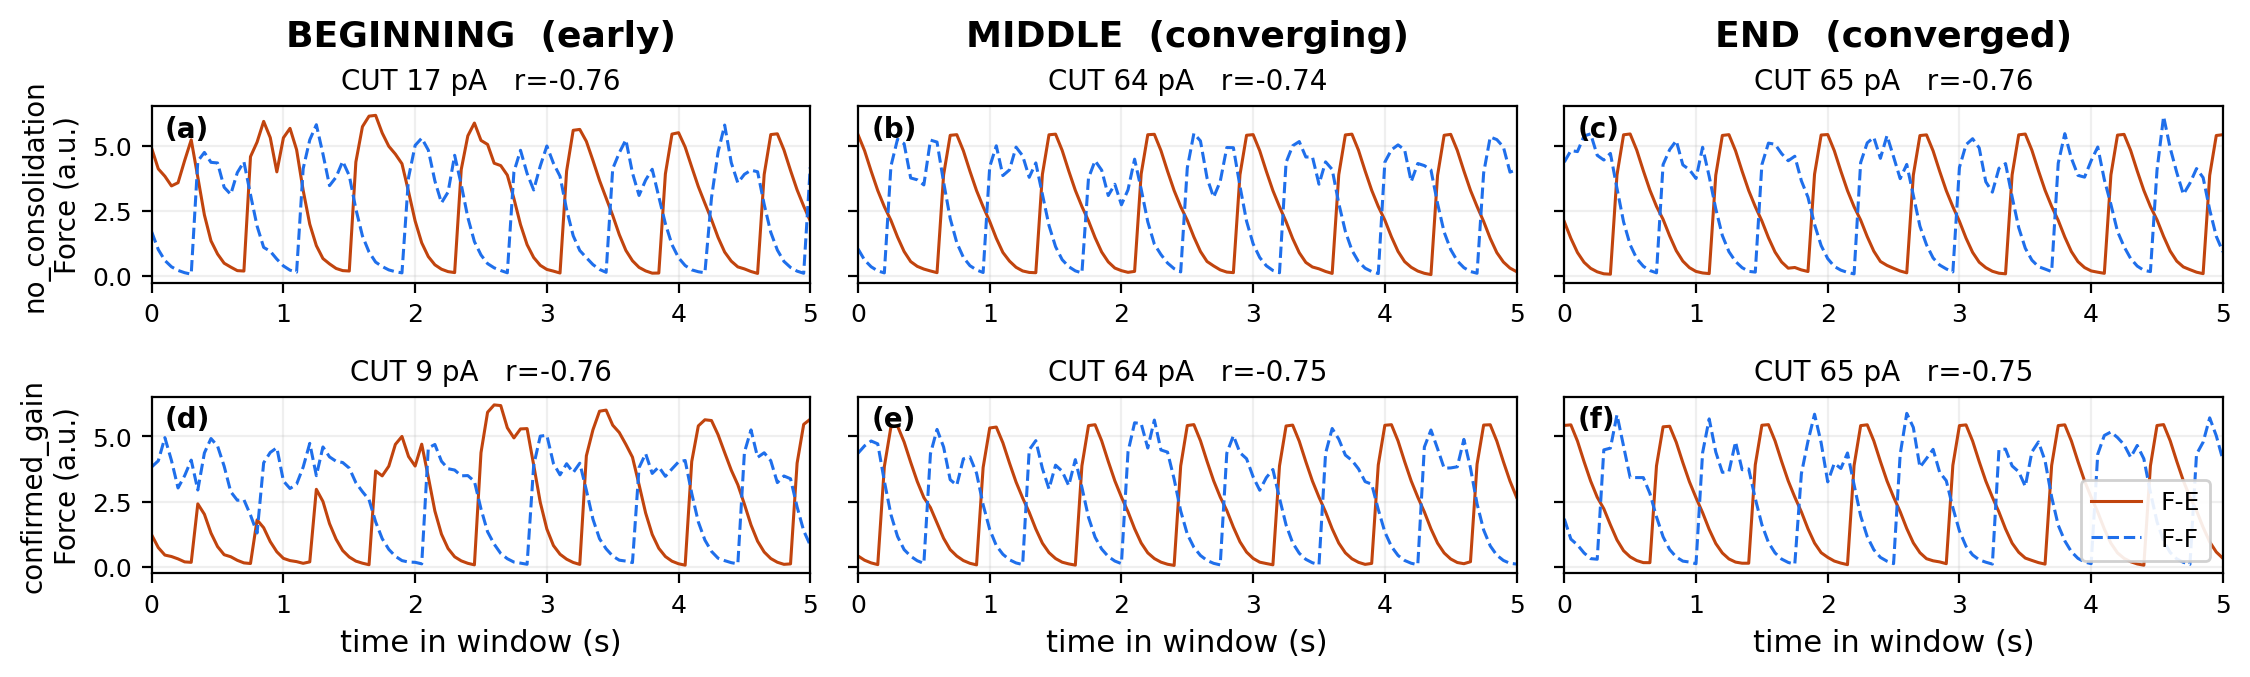
\includegraphics[width=0.92\textwidth]{fig_consolidate_sensory_force_stages.png}
  \caption{\textbf{Tag-and-capture consolidation, sensory arm.} Rows: no
    consolidation; the confirmed working gain ($0.25$ genuine / $0.10$
    forced --- the same setting as the descending arm). Columns as in
    Figure~\ref{fig:ct_all_modes_force}. Panels (a)--(f).}
  \label{fig:consolidate_sens}
\end{figure}

\begin{figure}[t]
  \centering
  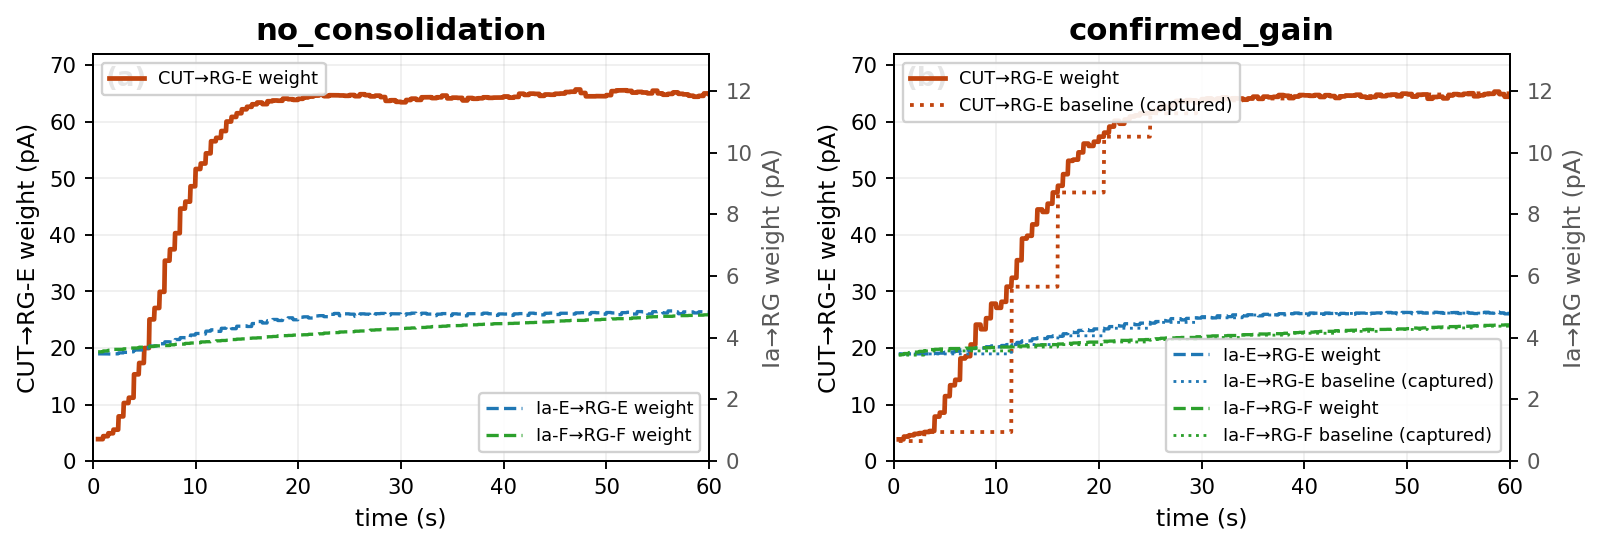
\includegraphics[width=0.95\textwidth]{fig_consolidate_sensory_weights_grid.png}
  \caption{\textbf{Same layout as Figure~\ref{fig:consolidate_desc_weights},
    sensory arm.} Left: no consolidation. Right: confirmed gain --- the
    cutaneous synapse's baseline steps upward and tracks the converged
    live weight, the same capture behavior seen in the descending arm.}
  \label{fig:consolidate_sens_weights}
\end{figure}

\paragraph{The same gain extends to the faster and toe-stepping timing
points once one further time constant is rescaled.} The gain search above
was run at the medium-speed timing point; naively applying the same
setting at the faster point or at toe stepping reproduced failure
signatures resembling those first documented for the sensory arm above
(failsafe domination or synchronization) even where the underlying
closed-loop timing itself was already genuine. The cause was a fixed leak
time constant governing how quickly an uncaptured tag relaxes back toward
its baseline: consolidation applies this leak continuously, not only
between captures, so a value tuned for the medium-speed cycle length
actively suppressed weight growth at the shorter cycle lengths of the
faster and toe-stepping points, independently of the gain. Rescaling this
one constant (roughly in proportion to how much faster the local cycle
is) restores the confirmed gain to genuine operation at both new points,
in both architectures. The three walking speeds are not uniformly clean,
however: fast reproduces as a near-identical cross-seed match (steady-state
corr$(F_{E,L},F_{E,R})$ within $0.001$ of itself across seeds), while toe's
anti-phase signal, though same-signed across seeds, is markedly weaker and
leaves a small residual failsafe-domination fraction on one leg --- a
genuine but less robust confirmation than fast's. The converged weight
trajectories for all three walking speeds are the ``medium'', ``fast'' and
``toe'' columns of Figure~\ref{fig:ct_all_modes_weights} above. The slow
walking point is the one exception found so far: the same rescaling
narrows but does not eliminate a residual left/right synchronization
tendency under consolidation, so Figure~\ref{fig:ct_all_modes_force}'s slow
rows run without consolidation (STDP alone, which is already excellent
there on its own) rather than with a setting confirmed to occasionally
misbehave.

\paragraph{Scope of this preliminary result.} This subsection now covers
four of the five locomotion modes under closed-loop timing (slow, medium,
fast walking and toe stepping), both learning architectures, and
tag-and-capture consolidation confirmed at three of those four (medium,
fast, toe) with a single shared gain. Slow alone runs consolidation-free,
by choice: the base mechanism is already excellent there on its own, and
consolidation was found actively harmful across a wide gain/threshold
search. Air stepping is deliberately excluded from the closed-loop-timing
and consolidation results, not because the mechanism fails to fit it, but
because a genuinely unloaded limb should not produce a clean closed-loop
rhythm at all --- see the discussion above and
Section~\ref{sec:results:epidural}. \todo{Revision note: everything in
this subsection, including the confirmed gain, is currently validated only
at reduced network size (debug scale); a full-scale confirmatory sweep
covering medium, fast and toe, both architectures, with consolidation
enabled at the confirmed gain, is in progress. Update this paragraph and
the preceding one once it lands --- do not cite the numbers above as
production-scale confirmed until then.}


\section{Discussion}\label{sec:discussion}
\subsection{Summary of contributions}
We extended a computational sCPG model --- a two-legged half-centre
network in the Hodgkin--Huxley lineage
running from Rybak 2006 through Shevtsova 2015 and Danner 2017 to
Zhang 2022~\cite{rybak2006,shevtsova2015,danner2017,zhang2022} --- with four
mechanisms absent from that lineage: (i)
STDP that lets the network tune its own
sensory-to-rhythm-generator synapses rather than have them hand-set; (ii) a
closed loop from muscle-force feedback (Ia) into the reciprocal-inhibition
core; (iii) motoneuron pools driving explicit muscle proxies with force and
length dynamics; and (iv) an externally paced cutaneous drive that emulates
heel-to-toe pressure transfer during stance. Using this model we asked how a
spinal CPG's own synaptic weights should be organised to produce a stable
walking rhythm, and how that self-tuned rhythm degrades as sensory feedback
is progressively withdrawn --- the central manipulation in rodent and human
studies of SCI rehabilitation.

Three findings anchor the paper. First, the three plastic synapses --- the
cutaneous CUT$\to$RG-E projection and the homonymous proprioceptive
projections Ia-E$\to$RG-E, Ia-F$\to$RG-F --- converge to the same steady
strength regardless of where they start, of which leg they are in, and of
walking speed (\autoref{sec:results:weights}); the network organises its own
descending gain rather than requiring it to be prescribed by the modeller.
Second, across the full grid of five locomotion modes and five learning
rates the quality of the alternating gait is not maximised by the fastest
learning, but peaks at an intermediate rate and falls off at both extremes
(\autoref{sec:results:comparison}). Third, removing load-dependent sensory
feedback and removing the cutaneous pacing drive have dissociable effects:
a model with only the pacing drive intact keeps stepping right through full
unloading, while a model in which both proprioceptive and cutaneous
feedback are gated by load collapses --- reproducing, in a spiking
closed-loop network, the clinical dissociation between unassisted and
epidurally-stimulated stepping after motor-complete SCI
(\autoref{sec:results:epidural}).

\subsection{Relation to prior computational and experimental sCPG work}
Zhang et al.\ (2022)~\cite{zhang2022} name two limitations of their own
four-rhythm-generator computational sCPG model explicitly: it has no
biomechanics or sensory feedback, and it has no motoneurons, treating
rhythm-generator output as a direct stand-in for motor output. Every
synaptic weight in their model, like its Rybak/Shevtsova/Danner
predecessors, is hand-tuned. Our model addresses both limitations for a
single hindlimb pair: the Ia force/length feedback loop supplies the
missing sensory closed loop, and explicit motoneuron pools driving a
saturating muscle model supply the missing motor periphery. On top of this
we add a mechanism none of these models have --- activity-dependent
plasticity on the afferent synapses --- so that the descending and
cutaneous gains are discovered by the network rather than fixed by the
experimenter.

The trade-off is architectural detail. Zhang et al.\ resolve genetically
identified commissural and long-propriospinal interneuron classes (V0V,
V0D, V1, V2a, V3, Shox2) across four limbs and reproduce V3-silencing
experiments quantitatively; our model collapses the commissural pathway to
two hand-set inhibitory projections between homologous half-centres and
covers only one limb pair. We also do not reproduce gait-transition
phenomena (walk $\to$ trot $\to$ gallop $\to$ bound): our gait is
externally paced rather than emergent from a single tonic-drive parameter.
The two efforts are complementary rather than competing: theirs
demonstrates architectural realism at the cost of a closed loop; ours
demonstrates a closed, self-organising loop at the cost of architectural
detail. A natural synthesis --- hand-curated interlimb architecture wrapped
in a plastic, closed sensorimotor loop --- is a direct extension of both.

Our loading manipulation and its epidural-stimulation analogue are drawn
directly from a second, experimental lineage: the rat and human
spinal-cord-injury work of Courtine, Lavrov, Edgerton, Gerasimenko and
colleagues showing that epidural stimulation of the lumbosacral spinal
cord can recover stepping across a graded series of load-bearing
conditions, from fully weight-supported walking to hindlimb
suspension~\cite{lavrov2008,edgerton2008,courtine2009,harkema2011}. That
literature establishes the phenomenon --- rhythmic electrical stimulation
of the cord restores stepping when descending drive is lost, in a
load-dependent manner --- largely from kinematic and electromyographic
readouts. Our model does not simulate the stimulation itself, but it
offers a mechanistic, spiking-network account of one candidate route to
the same phenomenon: a closed sensorimotor loop in which a rhythmic
afferent volley, held constant across loading, substitutes for the
load-gated sensory drive that unassisted stepping loses
(\autoref{sec:results:epidural}). In that sense the model is positioned to
connect the computational sCPG lineage above with this experimental
SCI-rehabilitation lineage, and we return to that connection in the
Clinical implications below.

\subsection{A shared mechanism underlies the learning-rate and loading
optima}
Two of our findings share the same underlying mechanism, which is worth
making explicit before turning to its clinical reading. Learning only
improves the gait once it has had time to organise the cutaneous weight
appropriately, and only within a specific range of final weight: at the
fastest rate ($\lambda=10^{-2}$) the descending weight overshoots useful
values and the alternation becomes slightly noisier, while at the slower
rates ($\lambda=10^{-5}, 10^{-6}$) the weight never gets there at all, so
the comparison across learning rates (\autoref{sec:results:comparison})
shows a broad optimum around $\lambda=10^{-3}$--$10^{-4}$ rather than a
monotonic benefit of faster learning. The same logic explains the
non-monotonic recovery we observe from toe to air stepping at slow learning
rates: an intermediate, partially-developed weight is poorly enough timed
to \emph{interfere} with the paced core's own alternation, whereas a fully
withdrawn afferent drive (air stepping) simply leaves the paced core to run
on its own, unperturbed floor. In both the learning-rate axis and the
loading axis, then, \emph{some} plastic drive organised correctly is better
than none, but a large, poorly-organised drive can be worse than either
extreme.

\subsection{Clinical implications}
The present computational approach yields several insights for the
clinical rehabilitation of individuals with SCI. Apart from recapitulating
locomotor behaviour, the proposed computational framework provides a
mechanistic account of how sensorimotor interactions and activity-dependent
plasticity might enable functional recovery. First, sensory inputs are
critical for facilitating locomotor rehabilitation, not as a replacement
for lost supraspinal descending input, but as a catalyst for plastic
adaptation in the spinal cord sensorimotor networks.

Our simulation results show that, when appropriately controlled through
load and/or activity, such sensorimotor input drives spinal adaptation and
subsequently restores coordinated locomotor outputs
(\autoref{sec:results:weights}).

Weight-bearing conditions fostered increasing potentiation of cutaneous
input and stabilisation of locomotor output, whereas reduced support
reduced sensory amplification and led to a more disorganised gait
(\autoref{sec:results:comparison}). These findings parallel clinical
observations that repetitive task-specific locomotor rehabilitation ---
body-weight-support treadmill walking, robot- and manually-assisted
stepping --- restores stepping in individuals with motor-incomplete SCI by
engaging residual plasticity in the spinal sensorimotor circuitry rather
than by regenerating damaged descending
pathways~\cite{wernigMuller1992,dietz1998,behrmanHarkema2000}. The model
provides a biologically plausible hypothesis for the benefits of epidural
stimulation in SCI. Reduced proprioceptive and exteroceptive inputs from
unloaded conditions resulted in poor locomotor performance.

The rhythmic input was, however, continuously driven by externally
delivered rhythmic cutaneous input, and these effects resulted in restored
alternating activity between flexors and extensors
(\autoref{sec:results:epidural}), a phenomenon observed in experiments in
animal models as well as in patients undergoing epidural stimulation of
the spinal cord~\cite{lavrov2008,edgerton2008,courtine2009,harkema2011}.

\paragraph{Which injury this model corresponds to.}
The two experimental manipulations map onto different points on the
clinical severity spectrum. The plasticity-driven weight-bearing arm
(\autoref{sec:results:weights}--\autoref{sec:results:comparison}) leaves
the brainstem-to-rhythm-generator (BS$\to$RG) drive tonic and non-zero
throughout, so it structurally represents a state in which some
supraspinal descending input survives the lesion --- clinically,
motor-incomplete SCI (ASIA Impairment Scale grades C/D), the population in
which BWSTT and robot- or manually-assisted training reliably restore
stepping~\cite{wernigMuller1992,dietz1998,behrmanHarkema2000}. Notably, the
synapses that are plastic in this arm, CUT$\to$RG-E and Ia$\to$RG, are not
the projections a thoracic or cervical lesion actually damages: those
afferent-to-interneuron connections are intraspinal and caudal to the
lesion, and do not cross it. What STDP models here is therefore not repair
of a severed pathway, but activity-dependent strengthening of an intact,
underused sensorimotor loop that compensates for reduced descending drive
--- the mechanism BWSTT and related therapies are thought to exploit. The
unloading/ESCS arm (\autoref{sec:results:epidural}), by contrast, models a
more severe injury in which even that residual drive is functionally
inadequate and an externally imposed rhythmic afferent volley substitutes
for it outright; this is closer to the regime in which epidural
stimulation is used clinically, often in motor-complete or near-complete
SCI where descending drive is minimal or absent~\cite{harkema2011}.

From this perspective, ESCS could function not just by increasing spinal
excitability, but by restoring or amplifying sensory signals necessary for
engaging the central pattern generators of the spinal cord to control
locomotion. Therefore, neuromodulation in SCI might be more efficient if it
is part of an integrated approach which includes not only electrical
stimulation, but also functionally relevant sensory stimuli. An additional
clinically relevant observation from our work is that the effectiveness of
recovery depends on the degree of plasticity.

Simulations reveal that intermediate levels of plasticity can produce more
robust, functional gait than very low or very high values ---
a range in which functional rehabilitation appears optimal, not maximised
(\autoref{sec:results:comparison}). The optimal levels of learning rate
would thus correspond to those that enable spinal cord motor networks to
adapt while avoiding extreme rewiring, and provide a useful heuristic guide
for determining appropriate intensities for rehabilitation and for
managing the effects of pharmacological or electrical neuromodulation
therapies on spinal adaptation. The optimal range of plasticity should be
dynamically adapted to each patient's neurophysiological state and
clinical characteristics.

\paragraph{Interpreting the learning-rate axis as plasticity capacity.}
One natural reading of the $\lambda$ axis is developmental. The capacity
for activity-dependent synaptic change is not fixed across the lifespan:
it is greatest during early postnatal critical periods and declines with
maturity, and correspondingly, neonatal and juvenile rodents recover
locomotor function after spinal injury considerably better than adults.
It is therefore tempting to read our fastest learning rates as
``younger'' and our slowest as ``older'' animals.\todo{cite developmental
critical-period / age-related decline in spinal plasticity and
age-dependent locomotor recovery after SCI} We suggest this analogy
should be treated as a qualitative ordering rather than a calibration:
$\lambda$ is a phenomenological STDP rate constant, it was not fitted to
any measurement of plasticity in animals of a given age, and age is only
one of several determinants of plasticity capacity --- time since injury,
prior activity history, and pharmacological or electrical neuromodulation
all modulate the same underlying quantity. Read this way, the $\lambda$
axis is better described as spanning \emph{plasticity capacity}, of which
age is one contributor.

With that caveat, the interpretation yields a concrete and testable
prediction. Because gait quality in our sweep peaks at intermediate
$\lambda$ rather than increasing monotonically
(\autoref{sec:results:comparison}), the model predicts that maximal
plasticity capacity is not automatically optimal for functional outcome
--- that a system rewiring too readily can be as poorly coordinated as one
that barely rewires at all. This resonates with the clinical picture in
which excessive or misdirected plasticity after SCI manifests as
maladaptive outcomes such as spasticity, aberrant sprouting and
neuropathic pain rather than improved locomotion.\todo{cite maladaptive
plasticity after SCI} The prediction is directly testable by running the
same rehabilitation protocol across age groups and asking whether
intermediate-age animals show the best coordination recovery, which would
be a stronger validation of the learning-rate axis than any of the
comparisons we are currently able to make.

Furthermore, the present computational framework might serve as a useful
tool for designing, optimising, and validating interventions before their
clinical application.

It is feasible to investigate, via simulation studies, various clinical
rehabilitation interventions (e.g., robot-assisted walking at various
assistance levels and weight-supported environments, ESCS at different
locations and frequencies, combination therapies) to identify the most
effective, non-invasive treatments. Finally, integrating this framework
with individual patient-specific data might pave the way for the
development of virtual-twin approaches that could predict, simulate, and
optimise patient outcomes after specific rehabilitation therapies in a
highly personalised fashion.

\subsection{Limitations}
In addition to the positive implications outlined above, it is important
to note some limitations of the proposed model. To simplify the biological
complexity of the spinal locomotor system, a level of abstraction was used
in defining sensorimotor pathways, interneurons and motor outputs. The
model does not include an adaptive supraspinal control mechanism (the
brainstem drive is a tonic input), detailed muscle-tendon
biomechanics beyond the saturating force/activation model used here,
fatigue, or other aspects of longer-term structural plasticity.

It also omits features of SCI such as chronic damage to the dorsal and
ventral roots, glial scarring, or the diversity of human SCI.

It should also be highlighted that the model was not calibrated on any
experimental data collected from actual individuals with SCI. Hence the
values of the STDP parameters can only be viewed as computational
representations of plasticity rather than direct measures of spinal
learning capacity. Consequently, the present model should be interpreted
as hypothesis-generating rather than predictive in nature, and further
studies incorporating more detailed muscle dynamics, more realistic
sensory transduction, supraspinal inputs, and patient-specific data will
be required to establish greater biological realism.

These conceptual limitations are compounded by several specific modelling
choices worth stating explicitly:

\begin{enumerate}
  \item \textbf{Interneuron and interlimb detail.} We resolve two hand-set
        commissural projections rather than the genetically identified
        V0/V1/V2a/V3 interneuron classes, and we model one hindlimb pair
        rather than fore--hindlimb coordination~\cite{zhang2022}; we
        likewise do not reproduce gait-transition phenomena
        (walk $\to$ trot $\to$ gallop $\to$ bound).
  \item \textbf{No stochastic replication.} Results are deterministic,
        fixed-seed point estimates; the ten-point initial-weight sweep
        (\autoref{sec:results:weights}) substitutes for repeated stochastic
        trials in establishing that a result is not an artefact of a
        particular initialisation.
\end{enumerate}

\subsection{Concluding remark}
A computational sCPG half-centre oscillator, closed in the loop with
motoneurons, muscle proxies, and load-dependent sensory feedback, tunes its
own descending gain through spike-timing-dependent plasticity to a stable
locomotor attractor --- one that is largely independent of how the network
starts, robust across the rat locomotor speed range, and best expressed at
an intermediate degree of plasticity rather than the maximum
achievable. Withdrawing load-dependent sensory feedback degrades that gait,
and restoring a rhythmic, load-independent afferent volley --- the model's
analogue of epidural stimulation --- rescues it, reproducing a central
dissociation in the SCI rehabilitation literature within a single
mechanistic, closed-loop model. Beyond the specific findings, the model
demonstrates that a spinal CPG's descending and sensory gains need not be
prescribed by the modeller: given a plastic synapse, appropriately timed
sensory drive, and enough time, the network finds them on its own. That
property, together with the model's explicit and inspectable parameters,
is what makes it a plausible substrate for exploring --- and eventually,
with patient-specific calibration, for helping to design --- sensorimotor
rehabilitation strategies after spinal cord injury.


% Supplementary material — delays table + algorithm pseudocode.
\clearpage
\section*{Supplementary material}

\subsection*{Supplementary Table: connectivity}
\begin{table}[t]
  \centering
  \footnotesize
  \caption{Distribution of synaptic weights and conduction delays along every
  projection, grouped by the architecture (Fig.~\ref{fig:schematic}). All
  projections carry per-connection weight \emph{distributions}: plastic
  projections (\textsuperscript{p}) from STDP / lognormal initialisation (CUT$\to$RG-E
  and Ia$\to$RG at their learned load set-points; BS$\to$RG frozen at weak init in the
  sensory arm), and static projections from imposed lognormal heterogeneity
  (CV$=0.5$, mean and sign preserved; Song 2005; Buzs\'aki \& Mizuseki 2014).
  Cutaneous input to RG-E is a single plastic projection. Delays follow the rat
  \texttt{length\_velocity} preset with $0.2$\,ms jitter. $n$ = connection count,
  leg L. Muscle$\to$Ia spindle feedback is rate-coded, not a synapse (no entry).}
  \label{tab:delays}
  \begin{tabular}{l r r r}
    \toprule
    Projection & $n$ & Weight (pA) & Delay (ms) \\
    \midrule
    \multicolumn{4}{l}{\textit{Descending / supraspinal drive}}\\
    \quad BS$\to$RG-E & 5070 & $+3.5\pm2.8$\textsuperscript{p} & $3.00\pm0.21$ \\
    \quad BS$\to$RG-F & 5041 & $+3.5\pm2.8$\textsuperscript{p} & $3.00\pm0.21$ \\
    \quad CUT$\to$RG-E (plastic) & 5003 & $+63.2\pm3.1$\textsuperscript{p} & $2.00\pm0.21$ \\
    \quad CUT$\to$InE & 1522 & $+6.0\pm3.1$ & $2.01\pm0.21$ \\
    \quad base$\to$RG-E & 978 & $+1.0\pm0.5$ & $2.99\pm0.21$ \\
    \quad base$\to$RG-F & 1007 & $+1.0\pm0.5$ & $2.99\pm0.21$ \\
    \addlinespace[2pt]
    \multicolumn{4}{l}{\textit{Sensory afferent $\to$ RG (plastic, sensory arm)}}\\
    \quad Ia-E$\to$RG-E & 5095 & $+4.4\pm0.3$\textsuperscript{p} & $2.00\pm0.21$ \\
    \quad Ia-F$\to$RG-F & 4880 & $+4.3\pm0.3$\textsuperscript{p} & $2.00\pm0.21$ \\
    \quad flexAff$\to$RG-F & 2522 & $+6.1\pm3.1$ & $2.00\pm0.21$ \\
    \quad flexAff$\to$InF & 1282 & $+5.9\pm2.9$ & $2.00\pm0.22$ \\
    \addlinespace[2pt]
    \multicolumn{4}{l}{\textit{Rhythm-generator reciprocal core}}\\
    \quad RG-E$\to$InE & 754 & $+11.8\pm5.9$ & $1.79\pm0.21$ \\
    \quad RG-F$\to$InF & 1490 & $+18.4\pm9.4$ & $1.80\pm0.21$ \\
    \quad InE$\to$RG-F & 768 & $-8.1\pm4.1$ & $1.80\pm0.21$ \\
    \quad InF$\to$RG-E & 1496 & $-48.0\pm24.5$ & $1.79\pm0.21$ \\
    \addlinespace[2pt]
    \multicolumn{4}{l}{\textit{Ia proprioceptive interneuron pathway}}\\
    \quad Ia-E$\to$IaInt-E & 1954 & $+5.9\pm2.9$ & $2.01\pm0.20$ \\
    \quad Ia-F$\to$IaInt-F & 1956 & $+6.0\pm3.0$ & $1.99\pm0.20$ \\
    \quad IaInt-E$\to$M-F & 2003 & $-10.1\pm5.1$ & $2.00\pm0.21$ \\
    \quad IaInt-F$\to$M-E & 1977 & $-10.3\pm5.1$ & $2.00\pm0.21$ \\
    \quad Ia-E$\to$InE & 1257 & $+6.1\pm2.9$ & $2.00\pm0.21$ \\
    \quad Ia-F$\to$InF & 1246 & $+5.8\pm2.9$ & $2.00\pm0.21$ \\
    \addlinespace[2pt]
    \multicolumn{4}{l}{\textit{Motor output}}\\
    \quad RG-E$\to$M-E & 4961 & $+30.1\pm15.0$ & $2.00\pm0.21$ \\
    \quad RG-F$\to$M-F & 5029 & $+29.8\pm14.4$ & $2.00\pm0.21$ \\
    \quad M-E$\to$M-F & 2510 & $-22.0\pm11.1$ & $1.80\pm0.21$ \\
    \quad M-F$\to$M-E & 2471 & $-22.0\pm11.1$ & $1.80\pm0.21$ \\
    \quad M-E$\to$mus-E & 7973 & $+1.0\pm0.5$ & $2.00\pm0.21$ \\
    \quad M-F$\to$mus-F & 7997 & $+1.0\pm0.5$ & $2.00\pm0.21$ \\
    \addlinespace[2pt]
    \multicolumn{4}{l}{\textit{Commissural (interlimb; abstracts V0v/V0d/V2a/In1)}}\\
    \quad commiss E (L$\to$R) & 1044 & $-7.9\pm4.0$ & $2.19\pm0.21$ \\
    \quad commiss F (L$\to$R) & 2177 & $-20.0\pm10.1$ & $2.20\pm0.21$ \\
    \addlinespace[2pt]
    \bottomrule
  \end{tabular}
\end{table}


\subsection*{Supplementary Algorithms: experimental protocols}

\begin{algorithm}[h]
\caption{Main experiment --- long-term self-organisation sweep over
$(\mu,\mathrm{CV})$.}\label{alg:main}
\begin{algorithmic}[1]
\Require Ten $(\mu_i,\mathrm{CV}_i)$ pairs from the ten $(\mu,\mathrm{CV})$ initialisation points; base seed $S_0=12345$
\Ensure Ten HDF5 files \texttt{cpg\_bursting\_paced\_120s\_idx<i>\_*.h5}
\For{$i \in \{0, 1, \dots, 9\}$ \textbf{in parallel} (SLURM array task $i$)}
  \State $\text{seed} \gets S_0 + 10007 \cdot i$
  \State Initialise STDP weights $w_{\text{init}} \sim \mathrm{Lognormal}(\mu_i, \mathrm{CV}_i)$
  \State Configure BS$=60$\,Hz tonic, paced gait
         (\verb|--step-period-ms 1000|, \verb|--n-ia-groups 3|, \verb|--ia-ext-hz 60 80 100|)
  \For{half-cycle $h = 0, 1, \dots, 239$ \Comment{$120$\,s / $500$\,ms}}
    \State $L \gets$ stance leg, $R \gets$ swing leg (alternates each $h$)
    \For{Ia sub-group $g \in \{0, 1, 2\}$} \Comment{heel, mid, toe}
      \State Set Ia-E rate of leg $L$, group $g$ to $\{60, 80, 100\}$\,Hz
      \State Simulate $167$\,ms; update activation, force, length, $r_{\text{Ia}}$ (Eq.~\ref{eq:ia})
      \State Sample STDP weights every $1000$\,ms; record force/RG-rate every $100$\,ms
    \EndFor
  \EndFor
  \State Write HDF5 with rates, weights, attrs (sim\_ms, $\mu_i$, $\mathrm{CV}_i$, seed, paced\_gait)
\EndFor
\end{algorithmic}
\end{algorithm}

\begin{algorithm}[h]
\caption{Phase A --- speed $\times$ STDP learning rate matrix.}\label{alg:speed_stdp}
\begin{algorithmic}[1]
\Require Operating point $(\mu, \mathrm{CV}) = (3.5, 0.30)$, $\mathrm{seed} = 12345$
\Ensure Nine HDF5 files \texttt{cpg\_speed\_stdp\_<spd>\_<lam>\_*.h5}
\For{$i \in \{0, 1, \dots, 8\}$ \textbf{in parallel} (SLURM array task $i$)}
  \State $\mathrm{speed\_idx} \gets \lfloor i / 3 \rfloor$;\ \ $\mathrm{lambda\_idx} \gets i \bmod 3$
  \State $P \gets \{1200,\ 520,\ 350\}[\mathrm{speed\_idx}]$ \Comment{ms; $\approx$ 6 / 13.5 / 21 cm/s}
  \State $\lambda \gets \{1{\times}10^{-5},\ 1{\times}10^{-4},\ 1{\times}10^{-3}\}[\mathrm{lambda\_idx}]$
  \State Configure paced gait with \verb|--step-period-ms|$=P$,
         \verb|--stdp-lambda|$=\lambda$
  \State Simulate $120$\,s at BS$=60$\,Hz with the standard 3-group Ia
         ramp (60, 80, 100\,Hz)
  \State Write HDF5 with \texttt{step\_period\_ms}=$P$, \texttt{stdp\_lambda}=$\lambda$
\EndFor
\State Report metrics over the last 20\,s of each cell: measured cycle
       period, peak Force-E, $\mathrm{corr}(F_E, F_F)$
\end{algorithmic}
\end{algorithm}

\begin{algorithm}[h]
\caption{Phase B --- graded Ia ablation $\times$ STDP learning rate
matrix (SCI-rehab paradigm).}\label{alg:ablgrad}
\begin{algorithmic}[1]
\Require Operating point $(\mu, \mathrm{CV}) = (3.5, 0.30)$,
$P=520$\,ms, $\mathrm{seed} = 12345$
\Ensure Nine HDF5 files \texttt{cpg\_ablgrad\_<gain>\_<lam>\_*.h5}
\For{$i \in \{0, 1, \dots, 8\}$ \textbf{in parallel} (SLURM array task $i$)}
  \State $\mathrm{gain\_idx} \gets \lfloor i / 3 \rfloor$;\ \ $\mathrm{lambda\_idx} \gets i \bmod 3$
  \State $G_{\text{Ia}} \gets \{1.0,\ 0.5,\ 0.1\}[\mathrm{gain\_idx}]$
         \Comment{baseline / toe step / air step}
  \State $\lambda \gets \{1{\times}10^{-5},\ 1{\times}10^{-4},\ 1{\times}10^{-3}\}[\mathrm{lambda\_idx}]$
  \State Configure paced gait with \verb|--step-period-ms|$=520$,
         \verb|--ia-feedback-gain|$=G_{\text{Ia}}$, \verb|--stdp-lambda|$=\lambda$
  \State Simulate $120$\,s; write HDF5 with the two new attrs
\EndFor
\State Report metrics over the last 20\,s of each cell: cycle period
       (mean $\pm$ s.d.), peak Force-E, $\mathrm{corr}(F_E, F_F)$
\end{algorithmic}
\end{algorithm}



% --- Data, code, reproducibility ---
\section*{Code and data availability}
All source code and the raw HDF5 simulation outputs underlying the figures in
this paper are available at
\href{https://github.com/max-talanov/tinyCPG}{github.com/max-talanov/tinyCPG}.

% --- Bibliography ---
\bibliographystyle{unsrt}   % switch to PLOS or Frontiers style at submission
\bibliography{refs}

\end{document}
